\documentclass[10pt]{article}
\usepackage{fullpage}
\usepackage{kcannon0}
\bibliographystyle{utphys}


\DeclareGraphicsRule{.fig.pdf}{pdf}{.fig.pdf}{}


\newcommand\lal{\textsc{lal}}
\newcommand\lalapps{\textsc{lalapps}}
\newcommand\ligotools{\textsc{ligotools}}

\newcommand{\prog}[1]{\texttt{#1}}
\newcommand{\function}[1]{\texttt{#1}}
\newcommand{\option}[1]{\texttt{#1}}
\newcommand{\parm}[1]{\textit{#1}}


\newenvironment{entry}%
{\begin{list}{}{\renewcommand{\makelabel}[1]%
{\parbox[b]{\labelwidth}{\makebox[0pt][l]{\textbf{##1}}\\}}%
\setlength{\labelwidth}{1em}%
\setlength{\labelsep}{1em}%
\setlength{\leftmargin}{2em}%
\setlength{\topsep}{\medskipamount}%
\setlength{\itemsep}{\medskipamount}%
\setlength{\parsep}{\medskipamount}%
\setlength{\listparindent}{0pt}}}
{\end{list}}


\title{Excess Power}
\author{Patrick Brady, Duncan Brown, Kipp Cannon, Saikat Ray-Majumder}
\date{2007-7-6}


\begin{document}
\maketitle


\section{Pipeline Overview}


The excess power pipeline implements an ``incoherent'' search for unmodeled
gravitational waves.  A schematic diagram of the data flow through the
pipeline is shown in Figure \ref{fig1}.
\begin{figure}
\begin{center}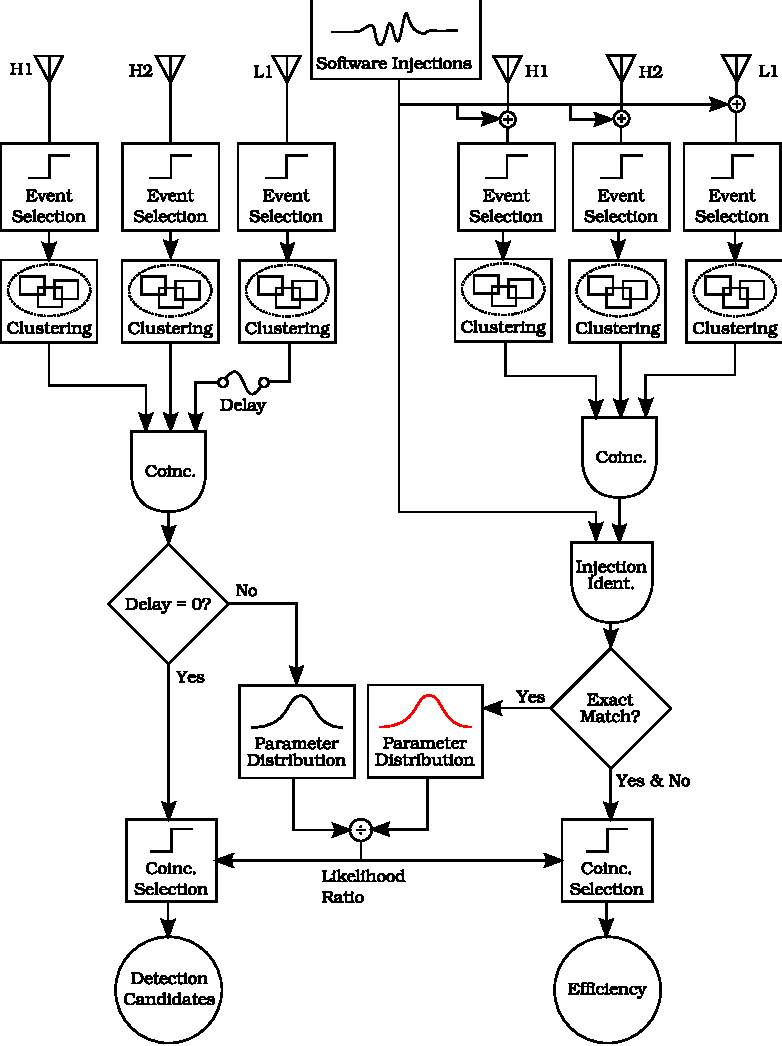
\includegraphics{figures/pipeline.pdf}\end{center}
\caption{Data flow in the excess power pipeline.  The dashed line marks the
division between the ``top half'' and ``bottom half'' of the pipeline (See
Section \ref{section2}).}
\label{fig1}
\end{figure}
Here and in what follows we'll discuss the multi-detector version of the
pipeline.  The pipeline can analyze any number of detectors, but in the 1
detector case much of the pipeline (e.g., the coincidence stages) reduces
to no-ops and is uninteresting.

The pipeline begins by scanning the outputs of the gravitational wave
detectors for statistically significant excursions from the background
noise.  In particular, it searches for excursions from the noise, or
bursts, that can be characterized by a frequency band and time interval.
The raw events identified in the outputs of the individual detectors are
clustered, which reduces the event rate and assists in parameter
estimation.  The clusters are tested for coincidence across instruments,
that is events are discarded unless matching events are also found in all
other detectors.  A set of events that, together, passes the coincidence
test will be refered to as a coincident \(n\)-tuple.

Prior to applying the coincidence test, optional delays can be applied to
the events.  In the LIGO-only case, delays are only applied to events from
the L1 detector.  The delay facility is used to collect two populations of
coincident \(n\)-tuples:  \(n\)-tuples with delays applied which are
refered to as time-slide coincidences, and \(n\)-tuples with no delays
applied which are refered to as zero-lag coincidences.

It is also possible to insert software injections into the detector time
series.  The injection facility is used to simulate the presense of
gravitational waves in the data.  When software injections are inserted
into the time series, the coincidence test is followed by an injection
identification step.  This stage identifies two populations of recovered
injections:  injections that are recovered very well, and injections that
are recovered poorly.

The time-slide non-injection \(n\)-tuples, and the \(n\)-tuples
corresponding to well-recovered software injections are collected together
and their parameters measured to yield two distribution density functions.
The parameter distribution density function measured from the time-slide
\(n\)-tuples is interpreted as the parameter distribution for noise-like
\(n\)-tuples, while the parameter distribution density function measured
from the software injections is interpreted as the parameter distribution
for gravitational wave-like \(n\)-tuples.  The ratio of these two
distributions is used to assign a likelihood ratio to each \(n\)-tuple.

Finally, a likelihood-ratio based threshold is applied to each \(n\)-tuple.
The zero-lag \(n\)-tuples that survive this final cut are gravitational
wave detection candidates.  The same cut is applied to software injection
\(n\)-tuples to measure the detection efficiency of the pipeline.  If the
final threshold is adjusted so that just exactly 0 zero-lag \(n\)-tuples
survive, the efficiency measured for the pipeline in that configuration can
be used to derive an upper-limit result.


\section{Program \prog{lalapps\_power}}


\subsection{Man Page}


\begin{entry}

\item[Name]
\prog{lalapps\_power} --- apply excess power event selection algorithm to
real or simulated gravitational wave detector data.

\item[Synopsis]
\prog{lalapps\_power} \newline \hspace*{0.5in}
\option{--bandwidth}~\parm{Hz} \newline \hspace*{0.5in}
[\option{--burstinjection-file}~\parm{file name}] \newline \hspace*{0.5in}
[\option{--calibrated-data}] \newline \hspace*{0.5in}
[\option{--calibration-cache}~\parm{cache file}] \newline \hspace*{0.5in}
\option{--channel-name}~\parm{string} \newline \hspace*{0.5in}
\option{--confidence-threshold}~\parm{threshold} \newline \hspace*{0.5in}
[\option{--debug-level}~\option{info|warn|error|off}] \newline \hspace*{0.5in}
[\option{--dump-diagnostics~\parm{XML filename}}] \newline \hspace*{0.5in}
\option{--filter-corruption}~\parm{samples} \newline \hspace*{0.5in}
\option{--frame-cache}~\parm{cache file} \newline \hspace*{0.5in}
[\option{--gaussian-noise-rms}~\parm{RMS}] \newline \hspace*{0.5in}
\option{--gps-end-time}~\parm{seconds} \newline \hspace*{0.5in}
\option{--gps-start-time}~\parm{seconds} \newline \hspace*{0.5in}
[\option{--help}] \newline \hspace*{0.5in}
\option{--high-pass}~\parm{Hz} \newline \hspace*{0.5in}
[\option{--inspiralinjection-file}~\parm{file name}] \newline \hspace*{0.5in}
\option{--low-freq-cutoff}~\parm{Hz} \newline \hspace*{0.5in}
[\option{--max-event-rate}~\parm{Hz}] \newline \hspace*{0.5in}
\option{--max-tile-bandwidth}~\parm{Hz} \newline \hspace*{0.5in}
\option{--max-tile-duration}~\parm{seconds} \newline \hspace*{0.5in}
[\option{--mdc-cache}~\parm{cache file}] \newline \hspace*{0.5in}
[\option{--mdc-channel}~\parm{channel name}] \newline \hspace*{0.5in}
[\option{--output}~\parm{file name}] \newline \hspace*{0.5in}
\option{--psd-average-points}~\parm{samples} \newline \hspace*{0.5in}
[\option{--ram-limit}~\parm{MebiBytes}] \newline \hspace*{0.5in}
\option{--resample-rate}~\parm{Hz} \newline \hspace*{0.5in}
[\option{--sim-cache}~\parm{cache file}] \newline \hspace*{0.5in}
[\option{--sim-seconds}~\parm{sec.s}] \newline \hspace*{0.5in}
[\option{--siminjection-file}~\parm{injection file}] \newline \hspace*{0.5in}
[\option{--seed}~\parm{seed}] \newline \hspace*{0.5in}
\option{--target-sample-rate}~\parm{Hz} \newline \hspace*{0.5in}
\option{--tile-stride-fraction}~\parm{fraction} \newline \hspace*{0.5in}
[\option{--user-tag}~\parm{comment}] \newline \hspace*{0.5in}
\option{--window-length}~\parm{samples} \newline \hspace*{0.5in}

\item[Description] 
\prog{lalapps\_power} performs an excess power analysis on real or
simulated data.  This program's input consists of gravitational wave
detector time series data, and an optional list of injections to add to the
time series prior to analysis.  The program's output is a list of events
identified as being statistically significant in the input time series.

Gravitational wave detector time series data is read from LIGO/VIRGO .gwf
frame files.  This program analyzes data from only a single detector at a
time, but it can analyze data that spans multiple frame files.  Usually a
collection of frame files is specified by providing as input to this
program a LAL cache file, as might be obtained from \prog{LSCdataFind}.

If software injections are desired, then a LIGO\_LW XML file containing a
sim\_burst table describing the software injections must also be provided
as input.  In the past it has also been possible to read sim\_inspiral
tables and MDC injection frame files, but these facilities have not been
tested in a long time.  See the \prog{lalapps\_binj} program described in
Sec.~\ref{program:lalapps-binj} for information on constructing injection
description files.

The output is written to a LIGO\_LW XML file containing a sngl\_burst table
listing the events found in the input time series.  The output file also
contains process, process\_params, and search\_summary tables containing
metadata describing the analysis that was performed.  In particular, these
other tables provide precise information about the instrument and interval
of time that the program analyzed.

By default, the output file is named following the standard frame file
naming convention.
\begin{quote}
\parm{instrument}-POWER\_\parm{comment}-\parm{start}-\parm{duration}.xml
\end{quote}
For example, if a search was run on the Hanford \(\unit{4}{\kilo\metre}\)
interferometer and generated triggers starting at GPS time
\(\unit{731488397}{\second}\), the triggers cover \(\unit{33}{\second}\)
after that time, and the command line includes the option
``\option{--comment} TEST'', then the file name would be 
\begin{quote}
H1-POWER\_TEST-731488397-33.xml
\end{quote}
The output file name can be set explicitly with the \option{--output}
command line option.  If the name ends in ``.gz'', then it will be
gzip-compressed.

\item[Options]\leavevmode
\begin{entry}
\item[\option{--bandwidth} \parm{Hz}]
Set the bandwidth in which the search is to be performed.  This must be an
integer power of 2.  This and the \option{--low-freq-cutoff} option
together set the frequency band to be searched.

\item[\option{--burstinjection-file} \parm{file name}]
Read the sim\_burst table from the LIGO\_LW XML file \parm{file name}, and
add the software injections described therein to the input time series
prior to analysis.

\item[\option{--calibrated-data}]
When the \option{--calibrated-data} option is supplied, input time series
data is read as IEEE double-precision samples.  Calibrated data, for
example from the GEO detector, or from LIGO's \(h(t)\) frames, is stored in
double-precision rather than single-precision format.  The default is to
read the data as IEEE single-precision samples, although internally the
code uses double precision throughout (single-precision input data is
re-quantized to double precision prior to processing).

\item[\option{--calibration-cache} \parm{cache file}]
Specify the location of calibration information.  \parm{cache file} gives
the path to a LAL-format frame cache file describing locations of
\texttt{.gwf} frame files that provide the calibration data ($\alpha$ and
$\beta$ coefficients) for the analysis.  Frame cache files are explained in
the ``framedata'' package in LAL.

\item[\option{--channel-name} \parm{string}]
Set the name of the data channel to analyze to \parm{string}.  This must
match the name of one of the data channels in the input frame files.  For
example, ``\verb|H2:LSC-AS_Q|''.

\item[\option{--confidence-threshold} \parm{threshold}]
Set the confidence threshold below which events should be discarded.  The
``confidence'' of an event is \(-\ln P(\text{event} | \text{stationary
Gaussian white noise})\), so an event with a confidence of 30 has a
probability of \(\ee^{-30}\) of having been found in stationary Gaussian
white noise.  For the LIGO instruments, a practical treshold is typically
around 10.

\item[\option{--debug-level} \option{info|warn|error|off}]
Sets the level of verbosity:  \option{info} = print all messages,
\option{warn} = print only warnings and errors, \option{error} = print only
errors, and \option{off} = be silent.  The default value is \option{error}.

\item[\option{--dump-diagnostics \parm{XML filename}}]
Dump diagnostic snapshots of internal time and frequency series data to a
LIGO Light Weight XML file of the given name.  The file is overwritten.

\item[\option{--filter-corruption} \parm{samples}]
The input time series data is passed through a conditioning filter prior to
analysis.  Generally, the conditioning filter should be expected to corrupt
some amount of the beginning and end of the time series due to edge
effects.  This parameter tells the code how much data, in samples, should
be ignored from the start and end of the time series.  A reasonable value
is 0.5 seconds worth of data.

\item[\option{--frame-cache} \parm{cache file}]
Obtain the locations of input \texttt{.gwf} frame files from the LAL frame
cache file \parm{cache file}.  LAL frame cache files are explained in the
``framedata'' package in LAL and can be constructed by running
\prog{LSCDataFind} on some systems.  One of \option{--frame-cache}, or
\option{--gaussian-noise-rms} must be specified.

\item[\option{--gaussian-noise-rms} \parm{RMS}]
If this parameter is provided instead of \option{--frame-cache}, then
Gaussian white noise will be synthesized and used as the input data.  One
of \option{--frame-cache}, or \option{--gaussian-noise-rms} must be
specified.

\item[\option{--gps-end-time} \parm{seconds}]
Set the GPS time up to which input data should be read.  Non-integer values
are permitted, but the fractional part must not contain more than 9 digits
(accurate to nanoseconds).

\item[\option{--gps-start-time} \parm{seconds}]
Set the GPS time from which to start reading input data.  Non-integer
values are permitted, but the fractional part must not contain more than 9
digits (accurate to nanoseconds).

\item[\option{--help}]
Display a usage message and exit.

\item[\option{--high-pass} \parm{Hz}]
The input time series is high-pass filtered as part of the input data
conditioning.  This argument sets the cut-off frequency for this filter.
In older versions of the program, this frequency was hard-coded to be
\unit{10}{\hertz} below the lower bound of the frequency band being
searched or \unit{150}{Hz}, which ever was lower.

\item[\option{--inspiralinjection-file} \parm{file name}]
Use \parm{file name} as a LIGO lightweight XML file containing a list of inspiral
injections to be made.   The file should contain a \verb+sim_inspiral+ table
which is used to set information about the types of inspiral injections to be made.
This file may be constructed by hand, the
\verb+lalapps_bbhinj+ program described in the Inspiral package   

\item[\option{--low-freq-cutoff} \parm{Hz}]
Set the lower bound for the frequency band in which to search for
gravitational waves.  This and the \option{--bandwidth} option together set
the frequency band to be searched.

\item[\option{--max-event-rate} \parm{Hz}]
Exit with a failure if the event rate, averaged over the entire analysis
segment, exceeds this limit.  This provides a safety valve to prevent the
code from filling up disks if the threshold is set improperly.  A value of
0 (the default) disables this feature.

\item[\option{--max-tile-bandwidth} \parm{Hz}]
This specifies the maximum frequency bandwidth, \(B\), that a tile can
have.  This also fixes the minimum time duration of the tiles, \(\Delta t =
1/B\).  This must be an integer power of 2.

\item[\option{--max-tile-duration} \parm{s}]
This specifies the maximum duration that a tile can have.  This also fixes
the minimum bandwidth of the tiles.  This must be an integer power of 2.

\item[\option{--mdc-cache} \parm{cache file}]
Use \parm{cache file} as a LAL format frame cache file describing the
locations of MDC frames to be used for injections.

\item[\option{--mdc-channel} \parm{channel name}]
Use the data found in the channel \parm{channel name} in the MDC frames for
injections.

\item[\option{--output} \parm{file name}]
Set the name of the LIGO Light Weight XML file to which results will be
written.  The default is
``\parm{instrument}-POWER\_\parm{comment}-\parm{start}-\parm{duration}.xml''.
Where \parm{instrument} is derived from the name of the channel being
analyzed, and \parm{comment} is obtained from the command line.
\parm{start} is the integar part of the GPS start time from the command
line, and \parm{duration} is the difference of the integer parts of the
GPS start and end times from the command line.

\item[\option{--psd-average-points} \parm{samples}]
Use \parm{samples} samples from the input time series to estimate the
average power spectral density of the detector's noise.  The average PSD is
used to whiten the data prior to applying the excess power statistic.  The
number of samples used for estimating the average PSD must be commensurate
with the analysis window length and analysis window spacing --- i.e.\ an
integer number of analysis windows must fit in the data used to estimate
the average PSD --- however this program will automatically round the
actual number of samples used down to the nearest integer for which this is
true.  This elliminates the need of the user to carefully determine a valid
number for this parameter, allowing him/her to instead select a number that
matches the observed length of time for which the instrument's noise is
stationary.

\item[\option{--ram-limit} \parm{MebiBytes}]
The start and stop GPS times may encompass a greater quantity of data than
can be analyzed at once due to RAM limitations.  This parameter can be used
to tell the code how much RAM, in MebiBytes, is available on the machine,
which it then uses to heursitically guess at a maximum time series length
that should be read.  The code then loops over the input data, processing
it in chunks of this size, until it has completed the analysis.  If this
parameter is not supplied, then the entire time series for the segment
identified by the GPS start and end times will be loaded into RAM.

\item[\option{--resample-rate} \parm{Hz}]
The sample frequency to which the data should be resampled prior to
analysis.  This must be a power of 2 in the range \unit{2}{\hertz} to
\unit{16386}{\hertz} inclusively.

\item[\option{--seed} \parm{seed}]
When synthesizing Gaussian white noise with \option{--gaussian-noise-rms},
this option can be optionally used to set the random number generator's
seed.

\item[\option{--tile-stride-fraction} \parm{fraction}]
This parameter controls the amount by which adjacent time-frequency tiles
of the same size overlap one-another.  This numeric parameter must be \(=
2^{-n}\), where \(n \in \mathrm{Integers}\).  A reasonable value is 0.5,
which causes each tile to overlap its neighbours in time by \(\frac{1}{2}\)
its duration and in frequency by \(\frac{1}{2}\) its bandwidth.

\item[\option{--user-tag} \parm{comment}]
Set the user tag to the string \parm{comment}.  This string must not
contain spaces or dashes (``-'').  This string will appear in the name of
the file to which output information is written, and is recorded in the
various XML tables within the file.

\item[\option{--window-length} \parm{samples}]
Set the number of samples to use for an analysis window to \parm{samples}.
Only the central half of the window will be analyzed, the first quarter and
last quarter of the window are used as padding to avoid corruption at
certain stages of the analysis.  For example, if you wish the code to
analyze the data in 1 second windows, you need to set this parameter to the
number of samples corresponding to 2 seconds of data.  This parameter must
be a power of 2.

\end{entry}


\item[Example]
To run the program, type:
\begin{verbatim}
lalapps_power \
--bandwidth 2048 \
--calibrated-data \
--channel-name "H1:LSC-STRAIN" \
--debug-level info \
--filter-corruption 4096 \
--frame-cache H-754008315-754008371.cache \
--gps-end-time 754008363 \
--gps-start-time 754008323 \
--high-pass 60.0 \
--low-freq-cutoff 70.0 \
--max-event-rate 10000 \
--psd-average-points 274432 \
--ram-limit 1024 \
--resample-rate 8192 \
--tile-stride-fraction 0.5 \
--user-tag testing \
--window-length 16384
\end{verbatim}
For this to succeed, the current directory must contain the file
\texttt{H-754008315-754008931.cache} describing the locations of the
\texttt{.gwf} frame files containing the channel \verb|H1:LSC-STRAIN|
spanning the GPS times 754008323.0 s through 754008363.0 s.

\item[Authors]
Patrick Brady, Saikat Ray-Majumder and Kipp Cannon.  
\end{entry}


\subsection{Time-Frequency Analysis Algorithm}


\subsubsection{Overview}


The Excess Power search method is motivated by the classical theory of
signal detection in Gaussian noise.  The method is the optimal search
strategy~\cite{anderson2001}, having only knowledge of the time duration
and frequency band of the expected signal,  but having no other information
about the power distribution in advance of detection.

The algorithm amounts to projecting the data onto a basis of test
functions, each of which is a prototype for the waveforms being sought in
the data.  The projection procedure is the following.  The input time
series is passed through a comb of frequency-domain filters, generating
several output time series, one each for a number of frequency channels.
Summing the squares of the samples in any one of these channels amounts to
summing the ``energy'' in the corresponding frequency band.  Summing only
the samples from a range of times produces a number that is interpreted as
the energy in that frequency band for that period of time --- the energy in
a time-frequency tile whose bandwidth is that of the frequency channel, and
whose duration is the length of the sum.

The search is a multi-resolution search, so tiles of many different
bandwidths and durations are scanned.  For performance purposes, only a
single frequency channel decomposition is used.  ``Virtual'' wide bandwidth
channels are constructed by summing the samples from multiple channels, and
correcting for the overlap between adjacent channel filters.

Once the energy in a tile has been measured, a threshold is applied to
select the ``important'' tiles.  The quantity thresholded on is the
probability of measuring at least that much energy in a tile with that
bandwidth and that duration in stationary Gaussian noise.  The procedure
employed to assess this probability is to first whiten and normalize the
data, to transform it into what is then assumed to be stationary white
unit-variance Gaussian noise, and then read off the probability of the
observed energy from a theoretical distribution derived from that
assumption.


\subsubsection{The Whitening Procedure}


Consider a discretely-sampled time-series of \(N\) samples, \(s_j\) where
\(0 \leq j < N\) and the sample period is \(\Delta t\).  Much of the signal
processing to be described below is done in the frequency domain, so the
first step is to multiply the time series by a window function, \(w_{j}\),
tapering it to 0 at the start and end to reduce the noise arising from the
data's aperiodicity at its boundary.  The mean square of the tapering
window's samples is
\begin{equation}
\sigma_{w}^{2}
   = \frac{1}{N} \sum_{j = 0}^{N - 1} w_{j}^2.
\end{equation}
Following multiplication by the tapering window, the data is Fourier
transformed to the frequency domain.  The complex amplitude of the
frequency bin \(k\) is
\begin{equation}
\tilde{s}_{k}
   = \frac{\Delta t}{\sigma_{w}} \sum_{j = 0}^{N - 1} w_{j} s_{j} \ee^{-2
   \pi \aye j k / N},
\end{equation}
where \(0 \leq k < N\).  The frequency bins \(\lfloor N / 2 \rfloor < k <
N\) correspond to negative frequency components, and are not stored because
the input time series is real-valued and so the negative frequency
components are redundant (they are the complex conjugates of the positive
frequency components).  For the non-negative frequencies, bin \(k\)
corresponds to frequency
\begin{equation}
f_{k}
   = k \Delta f,
\end{equation}
where the bin spacing is \(\Delta f = (N \Delta t)^{-1}\).  Defining the
power spectral density as
\begin{equation}
P_{k}
   = \Delta f \mean{\magnitude{\tilde{s}_{k}}^{2} + \magnitude{\tilde{s}_{N
   - k}}^{2}}
   = 2 \Delta f \mean{\magnitude{\tilde{s}_{k}}^{2}},
\end{equation}
for \(0 \leq k < \lfloor N / 2 \rfloor\), the ``whitened'' frequency series
is
\begin{equation}
\hat{s}_{k}
   = \sqrt{\frac{2 \Delta f}{P_{k}}} \tilde{s}_{k}
\end{equation}
so that
\begin{equation}
\label{eqn3}
\mean{\magnitude{\hat{s}_{k}}^2}
   = 1.
\end{equation}
The definition of the power spectral density is such that
\begin{align}
\mean{s_{j}^{2}}
   & = \frac{1}{N^{2} \Delta t^{2}} \sum_{k = 0}^{N - 1} \sum_{k' = 0}^{N -
   1} \mean{\tilde{s}_{k} \conj{\tilde{s}}_{k'}} \ee^{2 \pi \aye j (k - k')
   / N}
   \\
   & = \frac{1}{2 N \Delta t} \sum_{k = 0}^{N - 1} P_{k},
\end{align}
when the frequency components are independent (the input time series is a
stationary process).

If the original time series is stationary Gaussian noise, this construction
makes each frequency bin's real and imaginary parts Gaussian random
variables with variances of 0.5.  The definition of the power spectral
density and of the Fourier transform shown above both match those of the
LIGO Algorithm Library, as documented in LIGO-T010095-00-Z.  Figure
\ref{fig:shistogram} shows the distribution of the real and imaginary
components of \(\hat{s}_{k}\) obtained from a sample of \(h(t)\) taken from
the LIGO L1 instrument during S4.
\begin{figure}
\begin{center}
\resizebox{5.5in}{!}{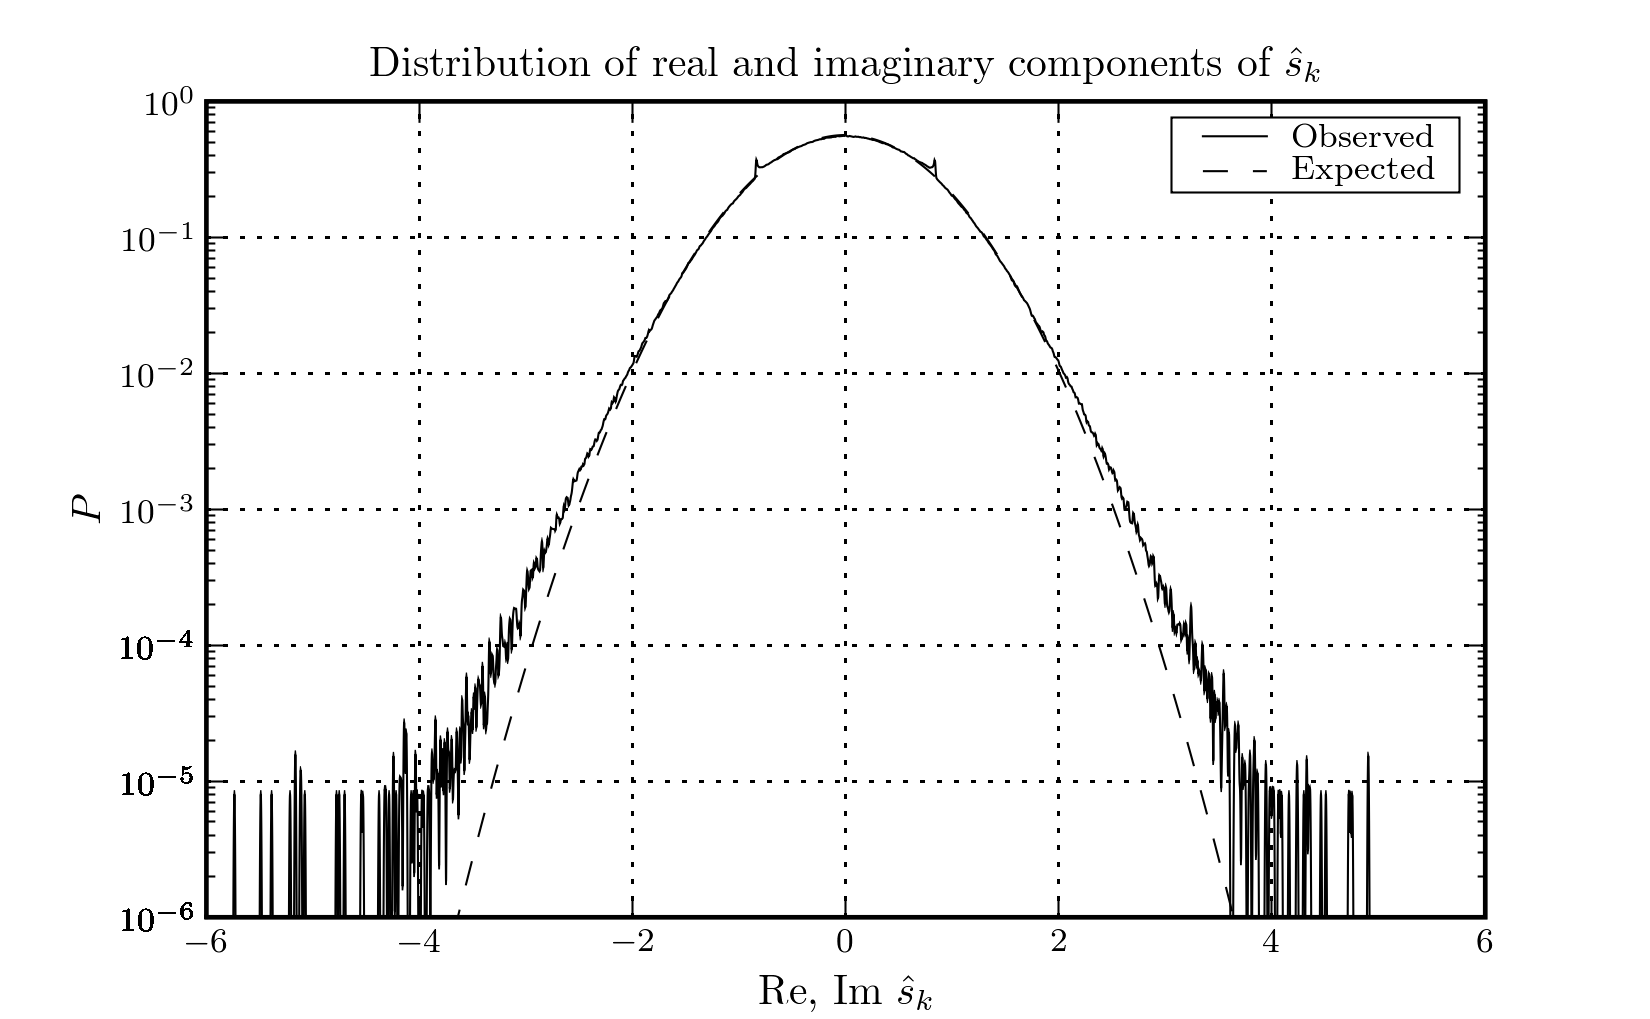
\includegraphics{figures/sk_histogram.png}}
\end{center}
\caption{The distribution of the real and imaginary components of
\(\hat{s}_{k}\) obtained from a sample of \(h(t)\) taken from the LIGO L1
instrument during S4.  The aparent bias away from the expected
normalization (actually non-Gaussianity) and the two horn features, are the
result of correlations between the power spectrum and the data.  Recall
that the power spectrum is estimated from the same data it is used to
whiten.}
\label{fig:shistogram}
\end{figure}

If the input time series is a stationary random process, then the
components of its Fourier transform are uncorrelated, and we would find
that \(\mean{\hat{s}_{k} \conj{\hat{s}}_{k'}} = \delta_{k k'}\).  However,
because we have windowed the time series (which is equivalent to convolving
its Fourier transform with that of the window), the frequency components
are now correlated.  We can compute \(\mean{\hat{s}_{k}
\conj{\hat{s}}_{k'}}\) by assuming the whitened time series consists of
independently-distributed random variables, because then the
Wiener-Khinchin theorem tells us that its two-point spectral correlation
function is the Fourier transform of its variance which we'll assume is
proportional to the square of the tapering window function.  Therefore,
\begin{equation}
\mean{\hat{s}_{k} \conj{\hat{s}}_{k'}}
   \propto \sum_{j = 0}^{N - 1} w_{j}^{2} \ee^{-2 \pi \aye j (k - k') / N}.
\end{equation}
The proportionality constant is obtained from \eqref{eqn3}, which tells us
that
\begin{equation}
\label{eqn4}
\mean{\hat{s}_{k} \conj{\hat{s}}_{k'}}
   = \frac{1}{\sigma_{w}^{2}} \sum_{j = 0}^{N - 1} w_{j}^{2} \ee^{-2 \pi
   \aye j (k - k') / N}.
\end{equation}
A comparison of this prediction to the observed two-point spectral
correlation in \(\hat{s}_{k}\) obtained from \(h(t)\) recorded at the LIGO
L1 instrument during S4 is shown in Figure \ref{fig:sksk}.
\begin{figure}
\begin{center}
\resizebox{5.5in}{!}{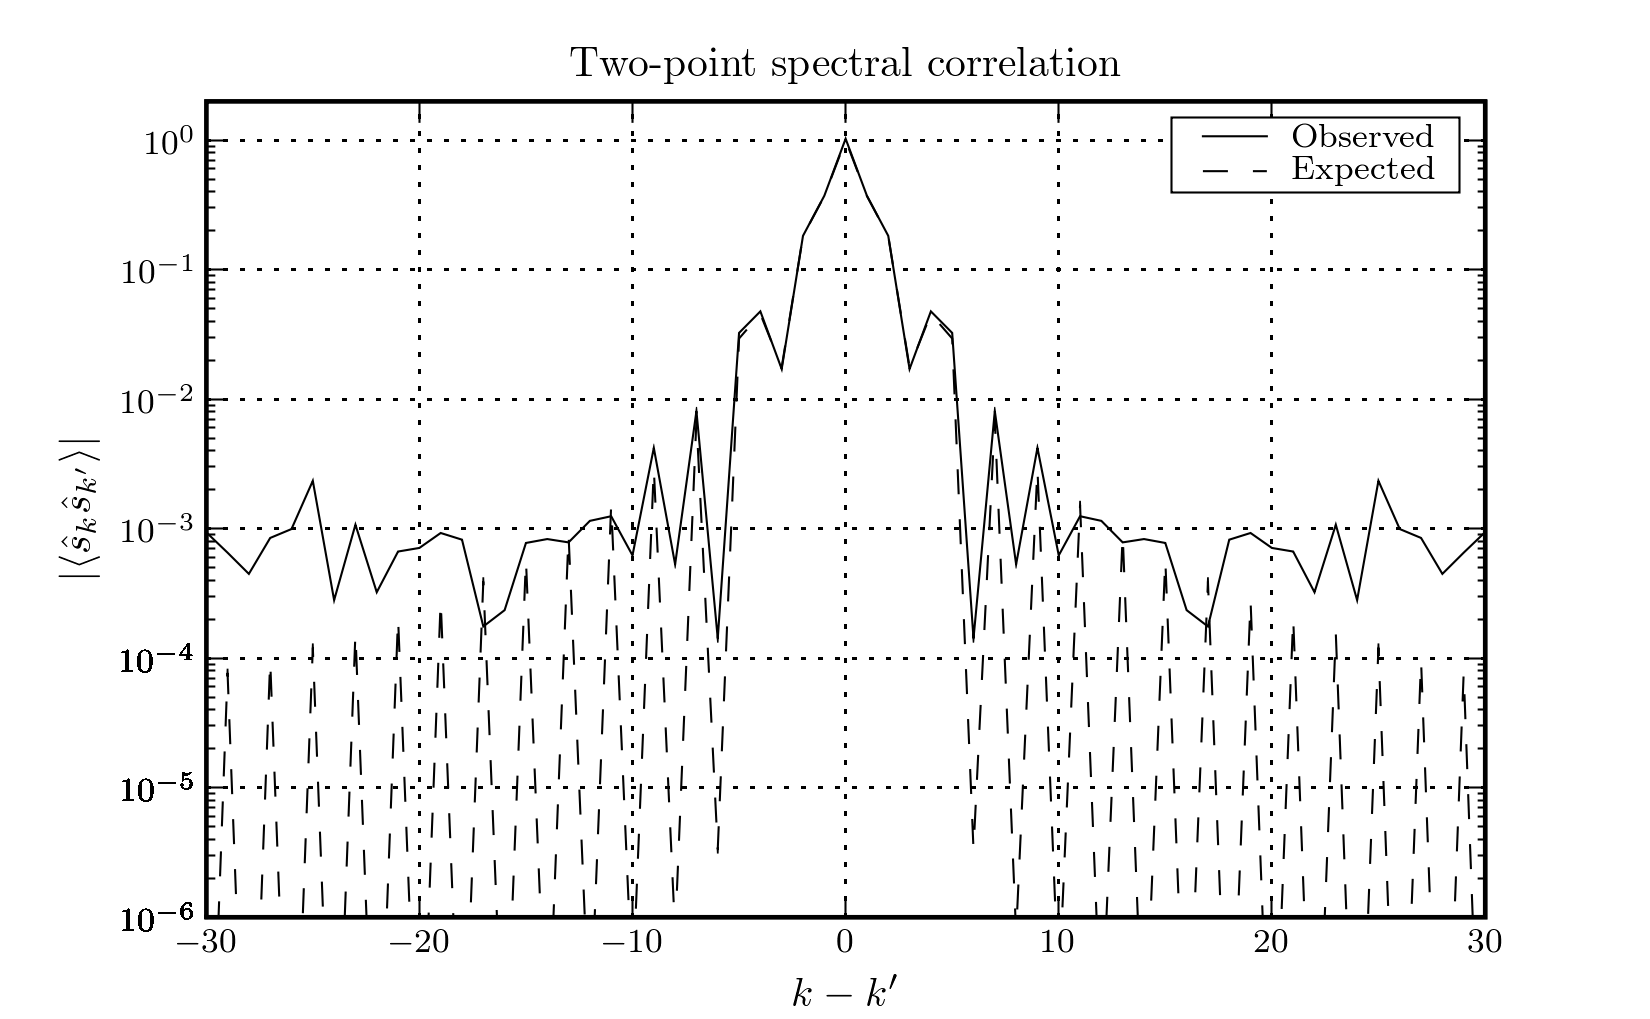
\includegraphics{figures/sksk.png}}
\end{center}
\caption{The two-point spectral correlation in the whitened data when a
Tukey window with 50\% flat top is used to taper the input time series.
The ``expected'' curve is what is expected in the limit of an average over
an infinite number of measurements.  Since a finite number of measurements
were made, a residual ``floor'' is expected, and it should go as
\((\text{number of measurements})^{-1/2}\).  Approximately 4 million
samples were averaged in each bin so the floor, which is
\(\mean{\hat{s}_{k} \conj{\hat{s}}_{k'}} \sim 2000^{-1}\), is consistent
with what is expected.}
\label{fig:sksk}
\end{figure}

The power spectral density is estimated using the median power at each
frequency for a number of overlapping segments.  The use of the median
avoids bias in the spectrum caused by the presence of a gravitational wave
or other large non-astrophysical transients present in any of the segments. 


\subsubsection{The Channel Filter}
\label{sec:channelfilter}


The choice of the channel filter is mostly irrelevant, except that it
correspond in some meaningful way to a particular frequency band.  We'll
denote the channel filter spanning frequencyes \(f_{1} \leq f_{k} < f_{2}\)
as \(\tilde{\Theta}_{k}(f_{1}, B)\), where the bandwidth of the filter is
\(B = f_{2} - f_{1}\).  If \(b\) is the bandwidth of the narrowest channel,
excess power achieves a multi-resolution search by computing only the
narrowest channels, and choosing
\begin{equation}
\tilde{\Theta}_{k}(f_{1}, n b)
   = \sum_{i = 0}^{n - 1} \Theta_{k}(f_{1} + i b, b),
\end{equation}
where \(B = n b\).  That is, the filters for wide band channels are chosen
to be the sums of adjacent filters from narrower bands.  The specific
choice made in excess power is to use Hann windows for the narrowest
channels.  The narrow channels are all the same width, and the Hann windows
are adjusted to be centred on their channel and extend over a range of
frequencies twice the width of the channel,
\begin{equation}
\tilde{\Theta}_{k}(f_{1}, b)
   \propto \begin{cases}
   \sin^{2} \frac{\pi}{2 b} (f_{k} - f_{1} + \frac{b}{2}), & f_{1} -
   \frac{b}{2} \leq f_{k} < f_{1} + \frac{3 b}{2} \\
   0, & \text{othewise}.
   \end{cases}
\end{equation}
In this way, when the filters for two adjacent channels are summed the
result is a Tukey window --- a window with a flat top in the middle and
\(\sin^{2}\) tapers at each end.

All windows are real-valued, so that they are phase preserving.  The
narrowest channel filters, the filters of bandwidth \(b\),  are normalized
so that
\begin{equation}
\label{eqn5}
\sum_{k = 0}^{N - 1} \sum_{k' = 0}^{N - 1} -1^{(k - k')} \mean{\hat{s}_{k}
\conj{\hat{s}}_{k'}} \conj{\tilde{\Theta}}_{k}(f_{1}, b)
\tilde{\Theta}_{k'}(f_{1}, b)
   = \frac{b}{\Delta f},
\end{equation}
where the two-point spectral correlation is given in \eqref{eqn4}.  The
reason for this choice will become clear later.  For convenience, let us
introduce the notation
\begin{equation}
\left\{ \tilde{X}, \tilde{Y} \right\}
   = \sum_{k = 0}^{N - 1} \sum_{k' = 0}^{N - 1} -1^{(k - k')}
   \mean{\hat{s}_{k} \conj{\hat{s}}_{k'}} \conj{\tilde{X}}_{k}
   \tilde{Y}_{k'},
\end{equation}
so
\begin{equation}
\left\{ \tilde{\Theta}(f_{1}, b), \tilde{\Theta}(f_{1}, b) \right\}
   = \frac{b}{\Delta f}.
\end{equation}
Notice that if the two-point spectral correlation is a Kroniker \(\delta\)
(the input data is not windowed), and the channel filter is flat,
\(\tilde{\Theta}_{k} = \tilde{\Theta}\), and spans the entire frequency
band from DC to Nyquist, \(b / \Delta f = N\), then the normalization would
lead to
\begin{equation}
\tilde{\Theta}
   = 1.
\end{equation}

In the LIGO Algorithm Library, the Fourier transforms of real-valued time
series contain only postive frequency components (the negative frequency
components being the complex conjugates of these), and so the channel
filters are also stored as only positive frequency components.  Since the
two-point spectral correlation function is usually strongly-peaked around
\(k - k' = 0\), and since the channel filters all go to zero far from the
DC and Nyquist components, in practice it is safe to sum over only the
positive frequency components, and require the sum to be
\begin{equation}
2 \sum_{k = 0}^{\lfloor N / 2 \rfloor + 1} \sum_{k' = 0}^{\lfloor N / 2
\rfloor + 1} -1^{(k - k')} \mean{\hat{s}_{k} \conj{\hat{s}}_{k'}}
\conj{\tilde{\Theta}}_{k}(f_{1}, b) \tilde{\Theta}_{k'}(f_{1}, b)
   = \frac{b}{\Delta f}.
\end{equation}
So the argument is that in practice this normalization is identical to
\eqref{eqn5}, but it is easier to implement because these are the only
components stored in memory.

For wide channels, channels formed by summing the filters from two or more
narrow channels, the ``magnitude'' of the channel filter will not be \(n b
/ \Delta f\).  For example,
\begin{equation}
\tilde{\Theta}_{k}(f_{1}, 2 b)
   = \tilde{\Theta}_{k}(f_{1}, b) + \tilde{\Theta}_{k}(f_{1} + b, b),
\end{equation}
and using the symmetry of \(\mean{\hat{s}_{k} \conj{\hat{s}}_{k'}}\) the
magnitude of this channel filter is found to be
\begin{align}
\left\{ \tilde{\Theta}(f_{1}, 2 b), \tilde{\Theta}(f_{1}, 2 b) \right\}
   & = \frac{2 b}{\Delta f} + 2 \left\{ \tilde{\Theta}(f_{1}, b),
   \tilde{\Theta}(f_{1} + b, b) \right\}.
\end{align}
The channel construction described above, with Hann windows for the
narrowest channels yielding Tukey windows for wider channels, allows us to
make the approximation that only adjacent channel filters have sufficient
overlap that their inner products are non-zero, and so the cross terms from
adjacent channels are the only ones that need to be accounted for.
Therefore, in general, a filter spanning \(n\) channels is
\begin{equation}
\tilde{\Theta}_{k}(f_{1}, n b)
   = \sum_{i = 0}^{n - 1} \tilde{\Theta}_{k}(f_{1} + i b, b),
\end{equation}
and its magnitude is
\begin{equation}
\left\{ \tilde{\Theta}(f_{1}, n b), \tilde{\Theta}(f_{1}, n b) \right\}
   = \frac{n b}{\Delta f} + 2 \sum_{i = 0}^{n - 2} \left\{
   \tilde{\Theta}(f_{1} + i b, b), \tilde{\Theta}(f_{1} + (i + 1) b, b)
   \right\}.
\end{equation}
Let us denote this magnitude as \(\mu^{2}(f_{1}, n b)\),
\begin{equation}
\label{eqn2}
\mu^{2}(f_{1}, n b)
   = \frac{n b}{\Delta f} + 2 \sum_{i = 0}^{n - 2} \sum_{k = 0}^{N - 1}
   \sum_{k' = 0}^{N - 1} -1^{(k - k')} \mean{\hat{s}_{k}
   \conj{\hat{s}}_{k'}} \tilde{\Theta}_{k}(f_{1} + i b, b)
   \conj{\tilde{\Theta}}_{k'}(f_{1} + (i + 1) b, b).
\end{equation}
When \(n = 1\), \(\mu^{2} = b / \Delta f\).

Figure \ref{fig:freqdomainfilter} illustrates the construction of a
\(\unit{16}{\hertz}\) channel filter from four \(\unit{4}{\hertz}\) channel
filters when \(\mean{\hat{s}_{k} \conj{\hat{s}}_{k'}} = \delta_{k k'}\).
\begin{figure}
\begin{center}
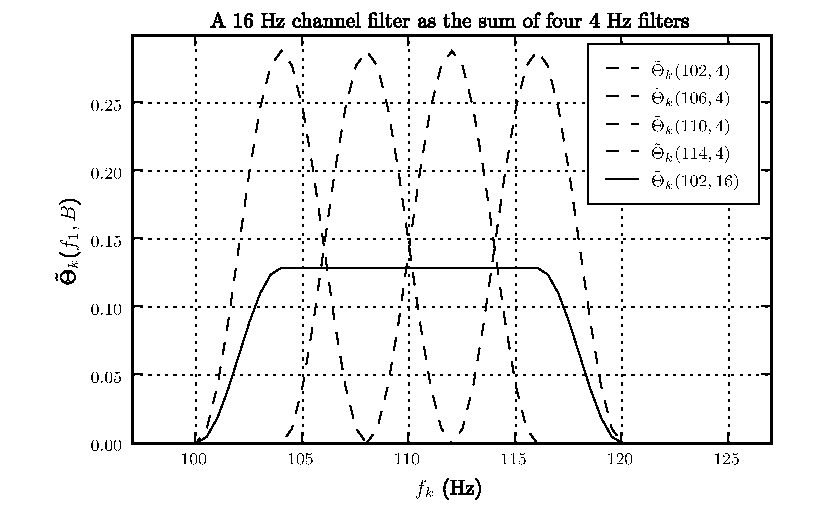
\includegraphics{figures/freqdomainfilter.pdf}
\end{center}
\caption{Summing narrow Hann channel filters to obtain wide-band Tukey
filters.}
\label{fig:freqdomainfilter}
\end{figure}
The \(\unit{16}{\hertz}\) channel filter has had its normalization adjusted
by the factor in \eqref{eqn2} to illustrate the relative amplitudes of the
channel filters when all are normalized to have magnitudes of 1.  This
figure also shows how the approximation that only adjacent channels have
non-zero overlap becomes exact in the limit of a two-point spectral
correlation function that is a Kroniker \(\delta\) (the ``tapering'' window
is flat, \(w_{j} = 1\)), because the third channel filter can only overlap
the first when there is mixing between \(k\).  The time-domain versions of
two sample channel filters are shown in Figure \ref{fig:timedomainfilter}.
\begin{figure}
\begin{center}
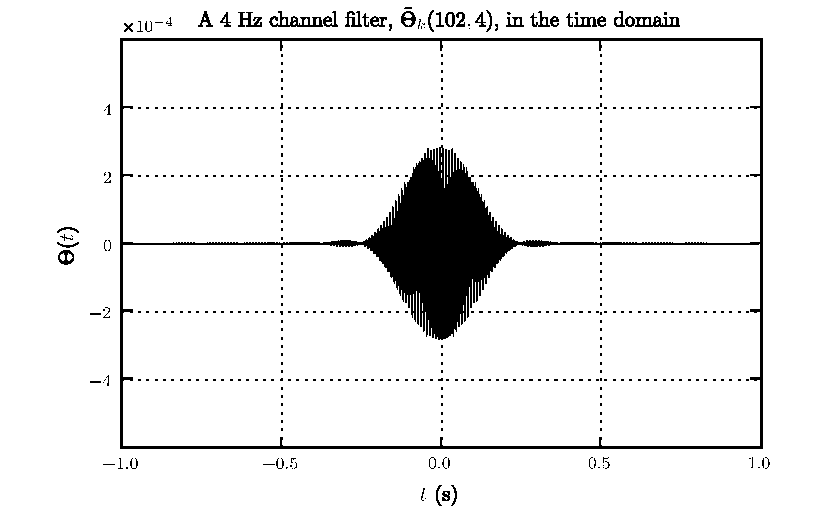
\includegraphics{figures/timedomainfilter_04hz.pdf}
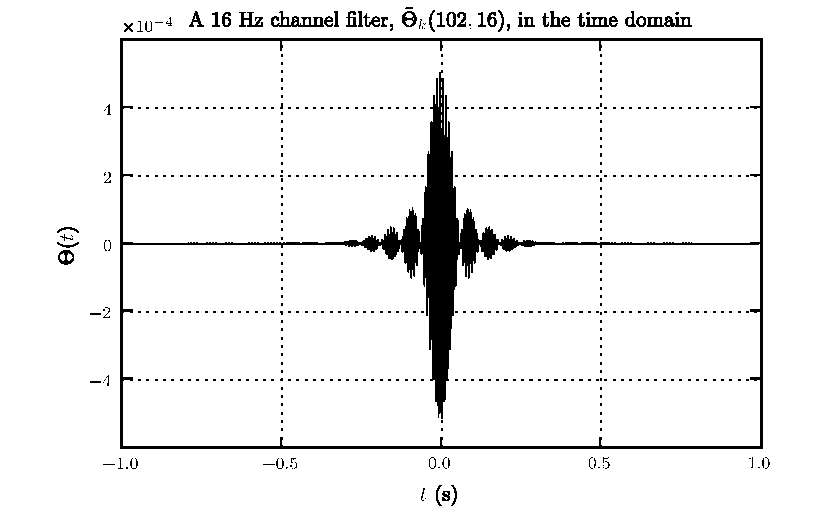
\includegraphics{figures/timedomainfilter_16hz.pdf}
\end{center}
\caption{Two examples of channel filters in the time domain.}
\label{fig:timedomainfilter}
\end{figure}


\subsubsection{The Channel Time Series}


The time series for a channel is extracted by multiplying the whitened
frequency-domain input data by the channel filter, and transforming the
result back to the time domain.  The time series for the channel of
bandwidth \(b\) starting at frequency \(f_{1}\) is
\begin{equation}
\label{eqn1}
z_{j}(f_{1}, b)
   = \frac{1}{N \Delta t} \sum_{k = 0}^{N - 1} \hat{s}_{k}
   \conj{\tilde{\Theta}}_{k}(f_{1}, b) \ee^{2 \pi \aye j k / N},
\end{equation}
and the mean square is
\begin{equation}
\mean{z_{j}^{2}(f_{1}, b)}
   = \frac{1}{N^{2} \Delta t^{2}} \sum_{k = 0}^{N - 1} \sum_{k' = 0}^{N -
   1} \mean{\hat{s}_{k} \conj{\hat{s}}_{k'}}
   \conj{\tilde{\Theta}}_{k}(f_{1}, b) \tilde{\Theta}_{k'}(f_{1}, b) \ee^{2
   \pi \aye j (k - k') / N}.
\end{equation}
The mean square is sample-dependent (depends on \(j\)) because the original
time series had the window \(w_{j}\) applied to it.  We will now require
that the window be of a kind with a flat portion in the middle, so that
\begin{equation}
w_{j}
   = \begin{cases}
   1 & \text{if \(0 \leq j_{1} \leq j < j_{2} \leq N\)},
   \\
   \leq 1 & \text{otherwise}.
   \end{cases}
\end{equation}
For example, a Tukey window is suitable.  In that case, the mean square of
\(z_{j}(f_{1}, b)\) should be independent of \(j\) when \(j_{1} \leq j <
j_{2}\).  If we further require the flat portion of the window to be in the
middle, in other words require \(j_{1}\) and \(j_{2}\) to be such that
\(j_{1} \leq N / 2 < j_{2}\), then we can pick \(j = N / 2\) as
representative of the mean square of \(z_{j}(f_{1}, b)\) in the flat
portion of the window.  Therefore,
\begin{equation}
\mean{z_{j}^{2}(f_{1}, b)}
   = \frac{1}{N^{2} \Delta t^{2}} \sum_{k = 0}^{N - 1} \sum_{k' = 0}^{N -
   1} -1^{(k - k')} \mean{\hat{s}_{k} \conj{\hat{s}}_{k'}}
   \conj{\tilde{\Theta}}_{k}(f_{1}, b) \tilde{\Theta}_{k'}(f_{1}, b).
\end{equation}
From the normalization of the channel filters (the motivation for the
formulation of which is now seen), the sum is \(b / \Delta f\), and
therefore
\begin{equation}
\mean{z_{j}^{2}(f_{1}, b)}
   = \frac{1}{N^{2} \Delta t^{2}} \frac{b}{\Delta f},
\end{equation}
for \(j_{1} \leq j < j_{2}\).

The LIGO Algorithm Library's \texttt{XLALREAL4ReverseFFT()} function
computes the inverse transform omitting the factor of \(\Delta f = 1 / (N
\Delta t)\) that appears in \eqref{eqn1}.  The time series returned by this
function is
\begin{equation}
Z_{j}(f_{1}, b)
   = N \Delta t z_{j}(f_{1}, b),
\end{equation}
and the mean squares of the samples in the time series are
\begin{equation}
\mean{Z_{j}^{2}(f_{1}, b)}
   = \frac{b}{\Delta f},
\end{equation}
for \(j_{1} \leq j < j_{2}\).  For a channel spanning \(n\) narrow
channels,
\begin{align}
Z_{j}(f_{1}, n b)
   & = \sum_{k = 0}^{N - 1} \hat{s}_{k} \conj{\tilde{\Theta}}_{k}(f_{1}, n
   b) \ee^{2 \pi \aye j k / N}
   \\
   & = \sum_{k = 0}^{N - 1} \hat{s}_{k} \left( \sum_{i = 0}^{n - 1}
   \conj{\tilde{\Theta}}_{k}(f_{1} + i b, b) \right) \ee^{2 \pi \aye j k /
   N}
   \\
   & = \sum_{i = 0}^{n - 1} Z_{j}(f_{1} + i b, b),
\end{align}
and so the samples in the time series for a wide channel are obtained by
summing the samples from the appropriate narrow channel time series.  The
mean squares of the samples of a wide channel's time series are given by
the quantity in \eqref{eqn2},
\begin{equation}
\mean{Z_{j}^{2}(f_{1}, n b)}
   = \mu^{2}(f_{1}, n b).
\end{equation}

Figure \ref{fig:Zhistogram} shows the distribution of \(Z_{j}(f_{1}, B)\)
observed in the same data used to measure the \(\hat{s}_{k}\) distribution
in Figure \ref{fig:shistogram}.
\begin{figure}
\begin{center}
\resizebox{5.5in}{!}{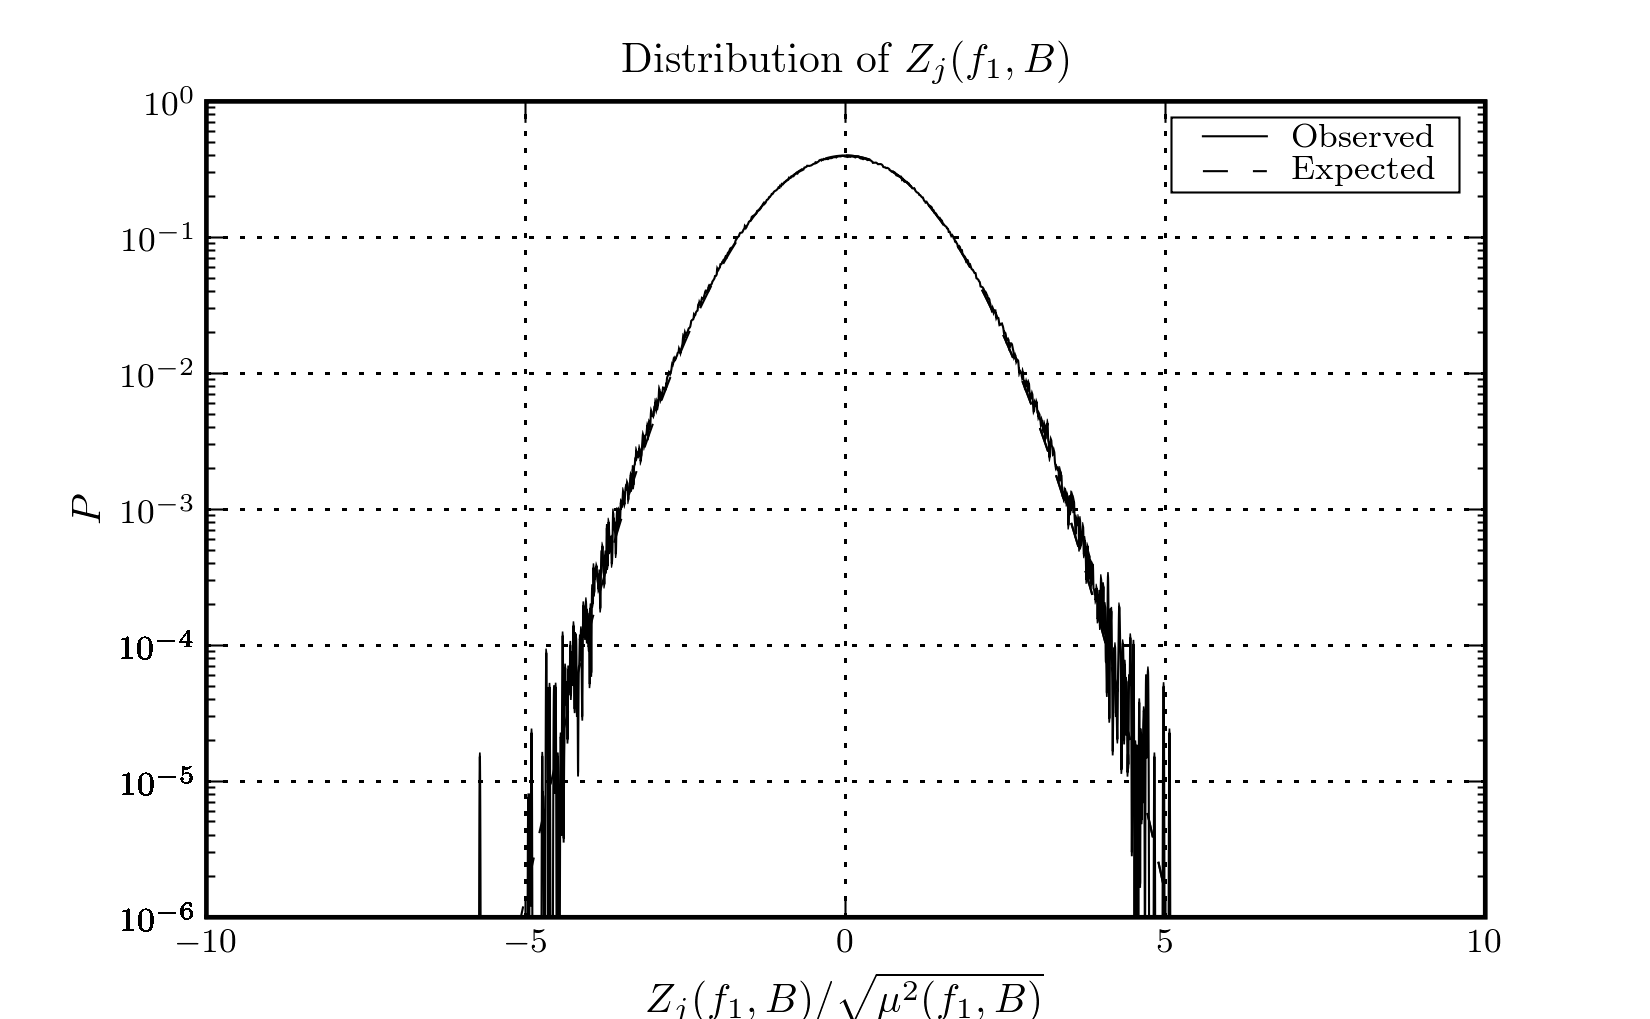
\includegraphics{figures/Z_histogram.png}}
\end{center}
\caption{The distribution of \(Z_{j}(f_{1}, B) / \sqrt{\mu^{2}(f_{1}, B)}\)
observed in data derived from a sample of \(h(t)\) taken from the LIGO L1
instrument during S4.  This distribution is measured from all samples used
to form time-frequency tiles.}
\label{fig:Zhistogram}
\end{figure}
This distribution appears more Gaussian than does the distribution of the
real and imaginary components of the whitened frequency series, and
generally exhibits better agreement with its expected behaviour.
Presumably this is a result of the central limit theorem:  the real and
imaginary components of the whitened frequency series may not be Gaussian,
but they do have unit variance, and since the time-domain samples of
\(Z_{j}\) are computed from many thousands of frequency bins, they end up
being unit variance Gaussian random variables.


\subsubsection{The Time-Frequency Tile}


Having projected the whitened input time series onto a comb of frequency
channels, including channels with a variety of widths, we now procede to
project it onto a collection of time-frequency tiles.  For this, we need to
know that the number of degrees of freedom in a tile of bandwidth \(B\) and
duration \(T\) is
\begin{equation}
d
   = 2 B T.
\end{equation}
This can be understood as follows.  A real-valued signal with a bandwidth
of \(B\) can be represented without loss of information as a discrete
real-valued time series with a sample rate equal to the Nyquist frequency
\(2 B\) (the time series may be a heterodyned version of the signal).
Therefore, \(2 B T\) real-valued samples are sufficient to encode all the
information contained in a signal of bandwidth \(B\) and duration \(T\).
We will require the number of degrees of freedom to be an even integer not
less than 2.

To construct the time-frequency tile spanning the frequencies \(f_{1} \leq
f < f_{1} + B\), and the times \(t_{1} \leq t < t_{1} + T\), we will use
the samples from the channel time series \(Z_{j}(f_{1}, B)\).  The channel
time series' sample period is \(\Delta t\), the same sample period as the
original input time series, but because the channel time series corresponds
to a more narrow frequency band than does the original input time series
(except in the special case of a channel spanning the entire input band),
there are more samples per unit time in the channel time series than there
are degrees of freedom per unit time --- the channel time series is over
sampled.  To obtain a time series with the correct sample rate, a sample
rate matching the actual number of degrees of freedom per second, we need
to down-sample the channel time series.

Let \(j_{1} = t_{1} / \Delta t\) be the time series sample index
corresponding to the start time of the tile.  The tile's duration spans a
total of \(T / \Delta t\) samples in the channel time series, but the tile
has \(d\) degrees of freedom so we need to down-sample the channel time
series so that from the \(T / \Delta t\) samples starting at \(j_{1}\) we
are left with \(d\) linearly independent numbers.  A simple down sampling
procedure is to select \(d\) evenly-spaced samples from the \(T / \Delta
t\) samples starting at \(j_{1}\).  Let these be the \(d\) samples at the
indices
\begin{equation}
\label{eqn8}
j
   = j_{1} + (i + \frac{1}{2}) \Delta j,
\end{equation}
where \(i = 0, \ldots, d - 1\), and \(\Delta j = T / (d \Delta t)\).  These
samples are linearly independent in the sense that it is not possible to
compute any one of them from the \(d - 1\) other samples, but they are
correlated because of the impulse response of the channel filter in the
time domain.  See, for example, Figure \ref{fig:timedomainfilter}.  In what
follows we will need the \(d\) samples forming the time-frequency tile to
be independent Gaussian random variables when the input time series is
stationary Gaussian noise.

Let us say that our \(d\) samples are the result of convolving the channel
impulse response with the ``real'' samples, and assume that if we
deconvolve the channel's impulse response from our samples we will be left
with \(d\) independent random variables.  The impulse response is
proportional to the inverse Fourier transform of the channel filter,
\begin{equation}
\Theta_{j}(f_{1}, B)
   = \frac{1}{N \Delta t} \sum_{k = 0}^{N - 1} \tilde{\Theta}_{k}(f_{1}, B)
   \ee^{2 \pi \aye j k / N}.
\end{equation}
Labeling the ``real'' samples as \(Z_{j}'(f_{1}, B)\), our assumption is
that our samples are derived from them by
\begin{equation}
\begin{bmatrix}
\vdots \\
Z_{j}(f_{1}, B) \\
\vdots
\end{bmatrix}
   \propto \begin{bmatrix}
   & \vdots & \\
   \cdots & \Theta_{j - j'}(f_{1}, B) & \cdots \\
   & \vdots &
   \end{bmatrix}
   \begin{bmatrix}
   \vdots \\
   Z_{j'}'(f_{1}, B) \\
   \vdots
   \end{bmatrix},
\end{equation}
where the \(j\) and \(j'\) indices are taken from \eqref{eqn8}.  Let's
write this matrix equation as
\begin{equation}
\vec{Z}(f_{1}, B)
   \propto \bar{\Theta}(f_{1}, B) \cdot \vec{Z}'(f_{1}, B).
\end{equation}
Inverting the equation gives the ``real'' samples in terms of our measured
samples,
\begin{equation}
\vec{Z}'(f_{1}, B)
   \propto \bar{\Theta}^{-1}(f_{1}, B) \cdot \vec{Z}(f_{1}, B).
\end{equation}
The proportionality constant is obtained by demanding that
\(\mean{Z_{j'}'^{2}(f_{1}, B)} = 1\).


\subsubsection{Excess Power (Energy)}


We define the whitened energy contained in the tile spanning the
frequencies \(f_{1} \leq f < f_{1} + B\) and the times \(t_{1} \leq t <
t_{1} + T\) as the sum of the squares of the down-sampled channel time
series
\begin{align}
E
   & = \frac{1}{\mu^{2}(f_{1}, B)} \vec{Z}(f_{1}, B) \cdot \vec{Z}(f_{1},
   B)
   \\
\label{eqn6}
   & = \frac{1}{\mu^{2}(f_{1}, B)} \sum_{i = 0}^{d - 1} Z_{j_{1} + (i +
   \frac{1}{2}) \Delta j}^{2}(f_{1}, B),
\end{align}
where \(j_{1} = t_{1} / \Delta t\) is the time series index corresponding
to the start of the tile, and \(\Delta j = T / (d \Delta t)\) is the number
of time series samples separating pixels in the time-frequency tile.

When the input time series is stationary Gaussian noise, \(E\) is the sum
of the squares of \(d\) Gaussian random variables each of whose mean is 0
and whose mean square is 1 (the factor of \(\mu^{2}\) normalizes them).
Therefore, \(E\) should be a \(\chi^{2}\)-distributed random variable of
\(d\) degrees of freedom.  Having measured an \(E\) for a tile, we can
calculate the probability that a tile would be found with at least that
\(E\) in stationary Gaussian noise, and threshold on this probability.  We
discard all tiles except those for which this probability is close to 0.
The tiling results in a large number of tiles being tested in every second
of data, and so a practical threshold is \(P(\geq E) \sim 10^{-7}\),
yielding an event rate of \(\unit{\order(\text{few})}{\hertz}\).  Figure
\ref{fig:ehistogram} shows a histogram of whitened tile energies observed
in the same strain data used to generate Figures \ref{fig:shistogram} and
\ref{fig:Zhistogram}.
\begin{figure}
\begin{center}
\resizebox{5.5in}{!}{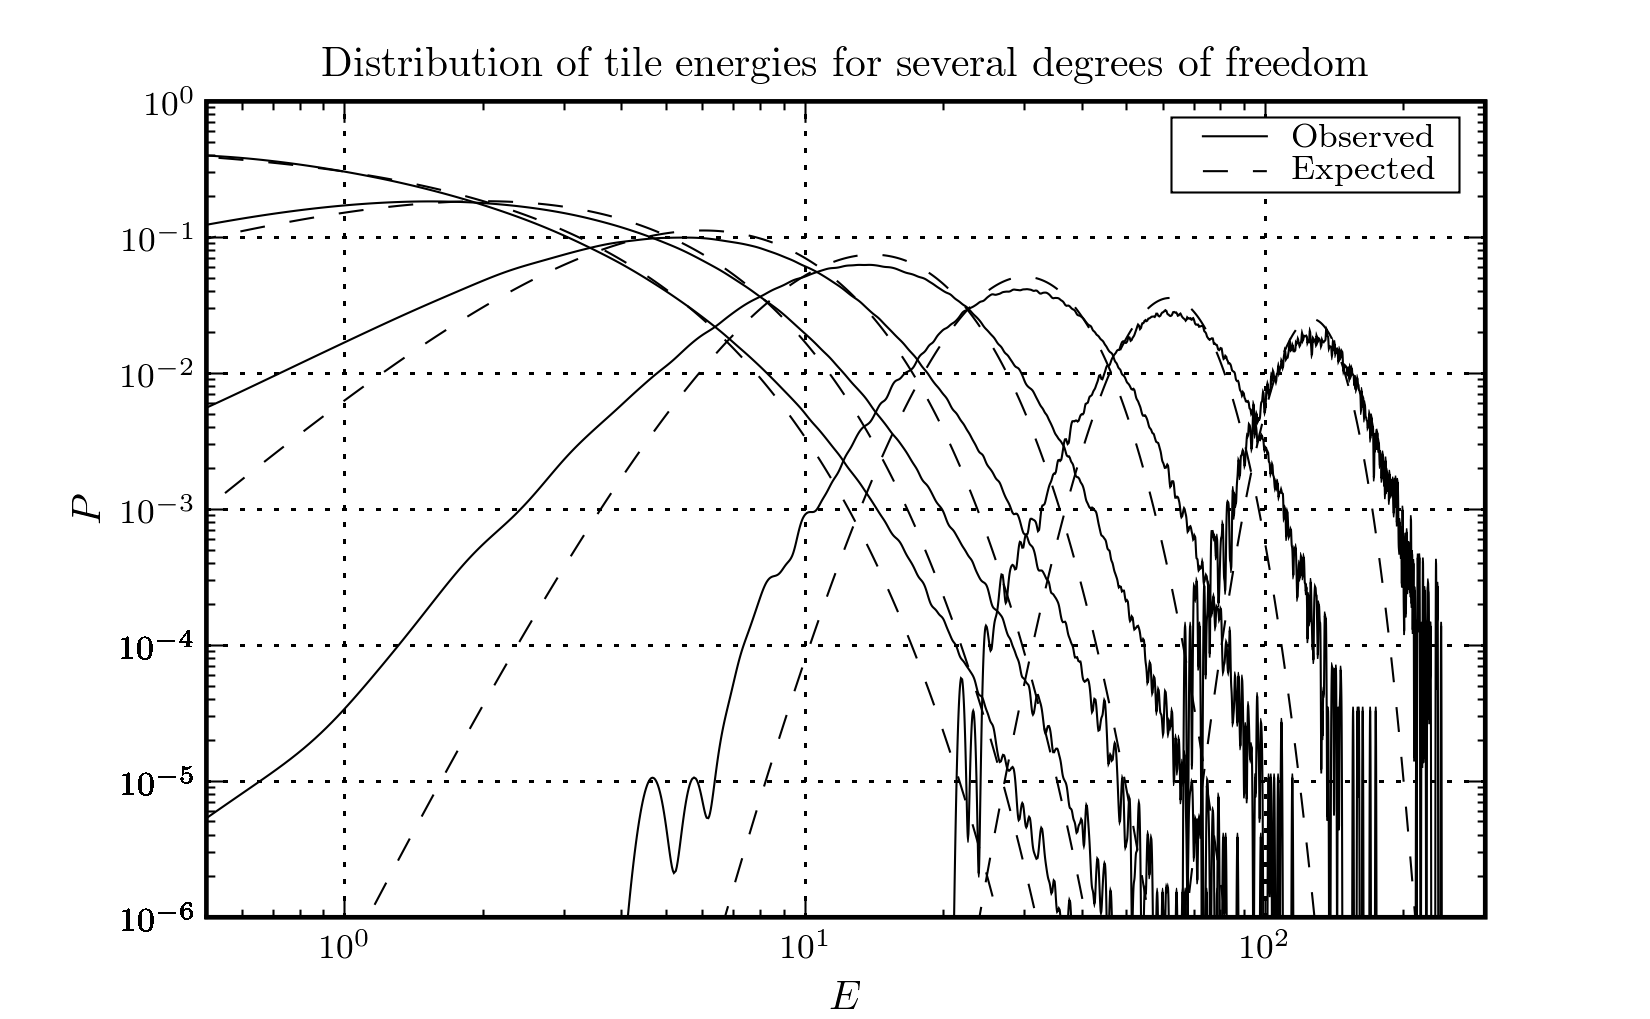
\includegraphics{figures/tiles_histogram.png}}
\resizebox{3.5in}{!}{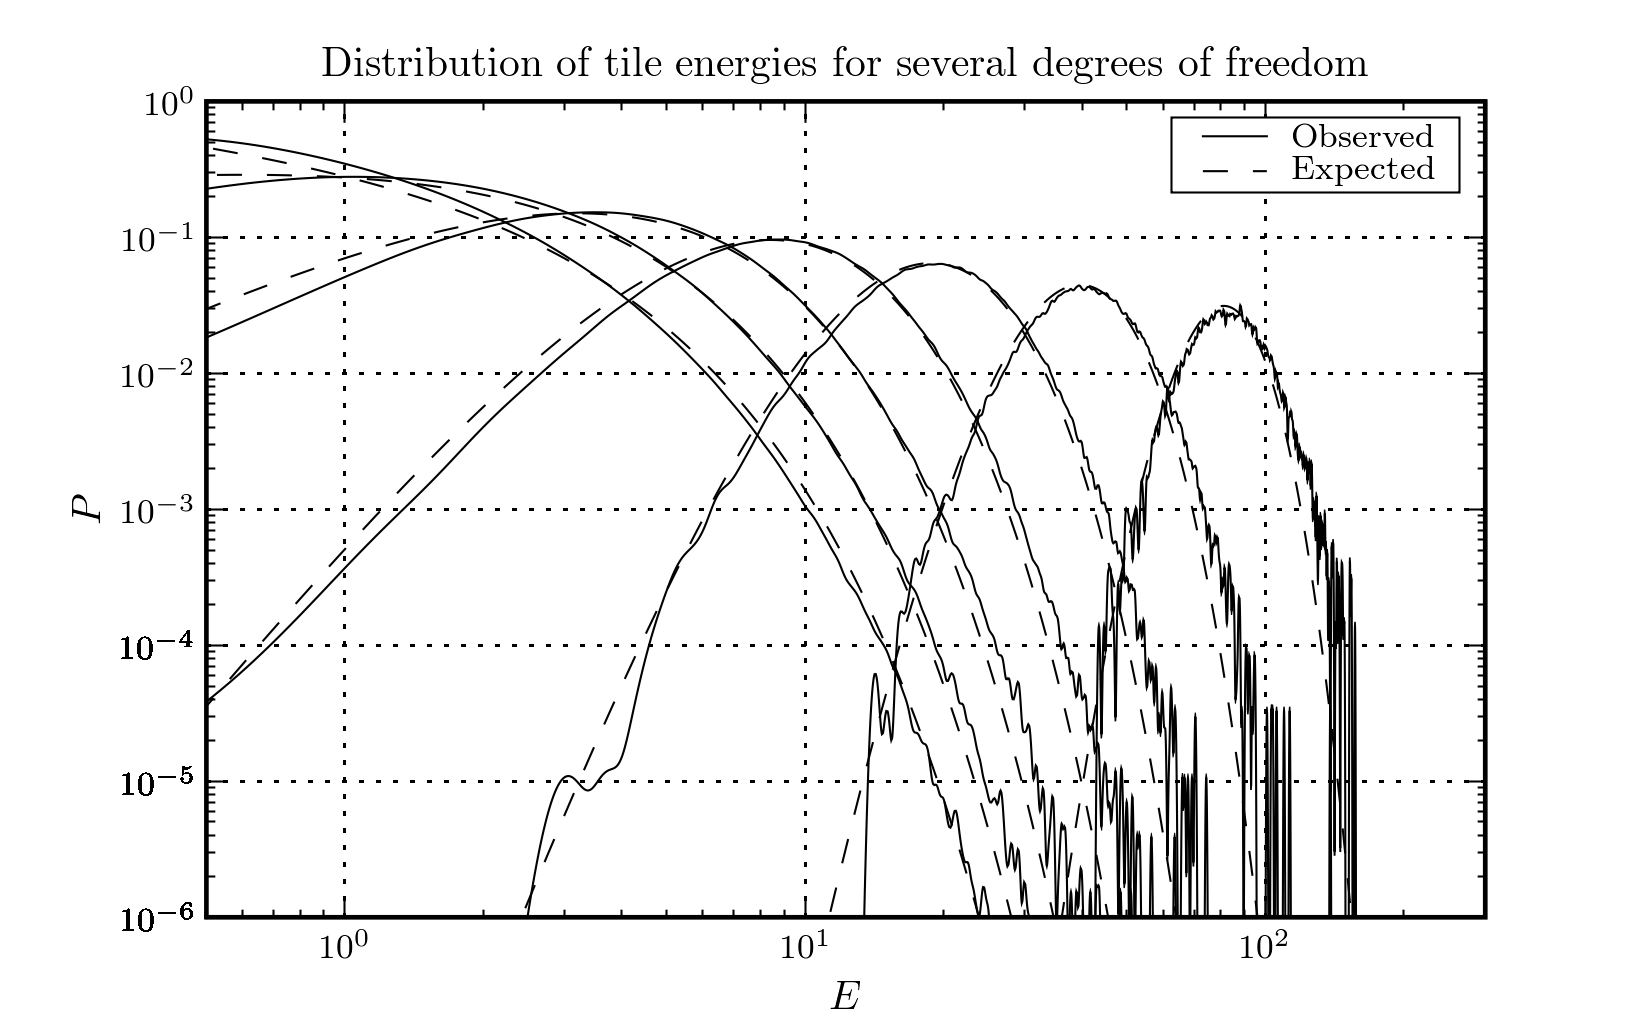
\includegraphics{figures/tiles_histogram_adjusted.png}}
\end{center}
\caption{The distribution of tile energies observed in a sample of \(h(t)\)
data collected from LIGO's L1 instrument during S4, the same data used to
obtain Figure \ref{fig:Zhistogram}.  The curves, in left-to-right order,
correspond to tiles with \(d = 2\), 4, 8, 16, 32, 64, and 128 degrees of
freedom.  The means appear to agree well with the expected values, but the
variances are little higher than expected.  This is consistent with the
tiles possessing fewer degrees of freedom than believed, which is
demonstrated in the smaller image where the energies and number of degrees
of freedom have been multiplied by 0.65, and the agreement has improved.
This is likely the result of the overlap of the channel responses in the
time domain.}
\label{fig:ehistogram}
\end{figure}

When a tile is identified as being unusual, the event is recorded in the
output file, and several properties of the event are measured and recorded.
One property is the ``confidence'', defined as
\begin{equation}
\text{confidence}
   = -\ln P(\geq E),
\end{equation}
the negative of the natural logarithm of the probability of observing a
tile with a whitened energy of \(E\) or greater in stationary Gaussian
noise.  This probability is typically close to 0, so the natural logarithm
is a large negative number, and the confidence a large positive number.
Larger ``confidence'' means a tile less like one would find in stationary
Gaussian noise.  A second quantity recorded for each event is the
signal-to-noise ratio (SNR).  The ``excess power'' (really excess energy),
of an event is
\begin{equation}
\text{excess power}
   = E - d.
\end{equation}
The expectation value of the whitened energy is \(\mean{E} = d\), so \(E -
d\) is the amount of whitened energy in the time-frequency tile beyond what
was expected --- the ``signal''.  Since the expected whitened energy is
\(d\), the SNR is
\begin{equation}
\rho
   = \frac{E - d}{d}.
\end{equation}


\subsubsection{Estimating \(h_{\text{rss}}\)}


The final quantity recorded for each event is the root-sum-squared strain,
or \(h_{\text{rss}}\).  We want the \(h_{\text{rss}}\) associated with a
particular time-frequency tile, and to do this we would like to have the
strain time series for the channel from which the time-frequency tile has
been constructed, \(h_{j}(f_{1}, B)\).  Unfortunately, we don't have this
information because we don't know what of the data is noise and what is
gravitational wave strain.  However, if we assume that the strain time
series and the noise time series are independent of one another, then the
mean square of data time series is the sum of the mean squares of the
strain and gravitational wave time series,
\begin{equation}
\mean{s_{j}^{2}(f_{1}, B)}
   = \mean{h_{j}^{2}(f_{1}, B)} + \mean{n_{j}^{2}(f_{1}, B)}.
\end{equation}
This is true on average, but we can use it to estimate the sum-of-squares
of \(h\) by summing the squares of \(s\) and subtracing the estimate of the
sum-of-squares of \(n\) derived from the measured power spectral density.
Essentially, we measure the ``energy'' in a time-frequency tile, and
subtract the mean noise energy to leave us with the gravitational wave
strain energy.  Therefore,
\begin{align}
\sum_{d} h_{j}^{2}(f_{1}, B)
   & = \left( \sum_{d} s_{j}^{2}(f_{1}, B) \right) - d
   \mean{n_{j}^{2}(f_{1}, B)}
   \\
   & = \left( \sum_{d} s_{j}^{2}(f_{1}, B) \right) - d
   \mean{s_{j}^{2}(f_{1}, B)}.
\end{align}
In this last line the notation has gotten a little confusing.  There is the
actual sum of squares of the data, and there is the expected sum of
squares.  We are using the (measured) mean square of the data in place of
the mean square of the noise on the assumption that it is noise that
dominates this quantity.  Also, \(\sum_{d}\) indicates the sum of \(d\)
time samples whose indices are the same as was used in \eqref{eqn6}.

The unwhitened time series corresponding to a single frequency channel is
the inverse Fourier transform of the unwhitened frequency series input data
multiplied by the corresponding channel filter,
\begin{align}
s_{j}(f_{1}, b)
   & = \frac{1}{N \Delta t} \sum_{k = 0}^{N - 1} \tilde{s}_{k}
   \conj{\tilde{\Theta}}_{k}(f_{1}, b) \ee^{2 \pi \aye j k / N}
   \\
   & = \frac{1}{N \Delta t \sqrt{2 \Delta f}} \sum_{k = 0}^{N - 1}
   \sqrt{P_{k}} \hat{s}_{k} \conj{\tilde{\Theta}}_{k}(f_{1}, b) \ee^{2 \pi
   \aye j k / N}
   \\
\label{eqn7}
   & = \frac{1}{\sqrt{2 N \Delta t}} \sum_{k = 0}^{N - 1} \sqrt{P_{k}}
   \hat{s}_{k} \conj{\tilde{\Theta}}_{k}(f_{1}, b) \ee^{2 \pi \aye j k /
   N}.
\end{align}
For a wide channel, \(\tilde{\Theta}_{k}(f_{1}, n b)\), we find just as for
\(Z_{j}(f_{1}, n b)\), that
\begin{equation}
s_{j}(f_{1}, n b)
   = \sum_{i = 0}^{n - 1} s_{j}(f_{1} + i b, b).
\end{equation}
The mean square of the unwhitened time series for a single channel is
\begin{equation}
\mean{s_{j}^{2}(f_{1}, b)}
   = \frac{1}{2 N \Delta t} \sum_{k = 0}^{N - 1} \sum_{k' = 0}^{N - 1}
   \sqrt{P_{k} P_{k'}} \mean{\hat{s}_{k} \conj{\hat{s}}_{k'}}
   \conj{\tilde{\Theta}}_{k}(f_{1}, b) \tilde{\Theta}_{k'}(f_{1}, b)
   \ee^{2 \pi \aye j (k - k') / N}.
\end{equation}
Making the same assumption as before, that the time series' mean square is
independent of the sample index \(j\) in the flat part of the input
tapering window, we can set \(j = N / 2\) inside the sum to leave us with
\begin{equation}
\mean{s_{j}^{2}(f_{1}, b)}
   = \frac{1}{2 N \Delta t} \sum_{k = 0}^{N - 1} \sum_{k' = 0}^{N - 1}
   -1^{(k - k')} \sqrt{P_{k} P_{k'}} \mean{\hat{s}_{k} \conj{\hat{s}}_{k'}}
   \conj{\tilde{\Theta}}_{k}(f_{1}, b) \tilde{\Theta}_{k'}(f_{1}, b).
\end{equation}
The double sum is a spectral density weighted version of the inner product
defined earlier for channel filters.  Introducing the notation
\begin{equation}
\left\{ X, Y; P \right\}
   = \sum_{k = 0}^{N - 1} \sum_{k' = 0}^{N - 1} -1^{(k - k')} \sqrt{P_{k}
   P_{k'}} \mean{\hat{s}_{k} \conj{\hat{s}}_{k'}} \conj{X}_{k} Y_{k},
\end{equation}
we can write the mean square as
\begin{equation}
\mean{s_{j}^{2}(f_{1}, b)}
   = \frac{1}{2 N \Delta t} \left\{ \tilde{\Theta}(f_{1}, b),
   \tilde{\Theta}(f_{1}, b); P \right\}.
\end{equation}
If we again make the assumption that only adjacent channels have any
significant non-zero overlap, then the mean square of the samples in an
unwhitened wide channel is
\begin{equation}
\mean{s_{j}^{2}(f_{1}, n b)}
   = \sum_{i = 0}^{n - 1} \mean{s_{j}^{2}(f_{1} + i b, b)} + \frac{1}{N
   \Delta t} \sum_{i = 0}^{n - 2} \left\{ \tilde{\Theta}(f_{1} + i b, b),
   \tilde{\Theta}(f_{1} + (i + 1) b, b) ; P \right\}.
\end{equation}

We need the \(s_{j}(f_{1}, n b)\) time series in order to compute the
unwhitened sum-of-squares for a particular tile, but constructing this time
series explicitly with the likes of \eqref{eqn7} incurs a factor of 2 cost
in both time and memory.  An approximation that works well in practice is
to assume that single channels of bandwidth \(b\) are sufficiently narrow
that the power spectral density is approximately constant in each one.
This allows \(P_{k}\) in \eqref{eqn7} to be replaced with some sort of
average and factored out of the sum to leave
\begin{equation}
s_{j}(f_{1}, b)
   \propto Z_{j}(f_{1}, b).
\end{equation}
The constant of proportionality is obtained from the known mean squares of
\(s_{j}(f_{1}, b)\) and \(Z_{j}(f_{1}, b)\), both of which are computed
(almost) without approximation.  Therefore,
\begin{equation}
s_{j}(f_{1}, b)
   \approx \sqrt{\frac{\Delta f}{b}} \sqrt{\mean{s_{j}^{2}(f_{1}, b)}}
   Z_{j}(f_{1}, b).
\end{equation}
We compute \(s_{j}(f_{1}, n b)\) for a wide channel by summing samples
across narrow channels,
\begin{equation}
s_{j}(f_{1}, n b)
   = \sum_{i = 0}^{n -1} s_{j}(f_{1} + i b, b) \propto \sqrt{\frac{\Delta
   f}{b}} \sum_{i = 0}^{n -1} \sqrt{\mean{s_{j}^{2}(f_{1} + i b, b)}}
   Z_{j}(f_{1} + i b, b),
\end{equation}
and again we solve for the proportionality constant from the ratio of the
mean squares of the left- and right-hand sides.  The mean square of the
left-hand side is given above, and that of the right-hand side is
\begin{multline}
\mean{\left( \sqrt{\frac{\Delta f}{b}} \sum_{i = 0}^{n -1}
\sqrt{\mean{s_{j}^{2}(f_{1} + i b, b)}} Z_{j}(f_{1} + i b, b) \right)^{2}}
   = \sum_{i = 0}^{n -1} \mean{s_{j}^{2}(f_{1} + i b, b)} \\+ \frac{2
   \Delta f}{b} \sum_{i = 0}^{n - 2} \sqrt{\mean{s_{j}^{2}(f_{1} + i b, b)}
   \mean{s_{j}^{2}(f_{1} + (i + 1) b, b)}} \left\{ \tilde{\Theta}(f_{1} + i
   b, b), \tilde{\Theta}(f_{1} + (i + 1) b, b) \right\}.
\end{multline}
Denoting the ratio as
\begin{equation}
\Upsilon^{2}(f_{1}, n b)
   = \mean{s_{j}^{2}(f_{1}, n b)} \mean{\left( \sum_{i = 0}^{n -1}
   \sqrt{\mean{s_{j}^{2}(f_{1} + i b, b)}} Z_{j}(f_{1} + i b, b)
   \right)^{2}}^{-1},
\end{equation}
the approximate unwhitened time series is
\begin{equation}
s_{j}(f_{1}, n b)
   \approx \sqrt{\Upsilon^{2}(f_{1}, n b)} \sqrt{\frac{\Delta f}{b}}
   \sum_{i = 0}^{n -1} \sqrt{\mean{s_{j}^{2}(f_{1}, b)}} Z_{j}(f_{1}, b).
\end{equation}
Figure \ref{fig:sjhistogram} shows a comparison of the distribution
observed in the samples of the approximate unwhitened time series
\(s_{j}(f_{1}, n b)\) values, for all bandwidths, as derived from the same
sample of \(h(t)\) recorded at the LIGO Livingston L1 instrument during S4
that has been used for the other plots.
\begin{figure}
\begin{center}
\resizebox{5.5in}{!}{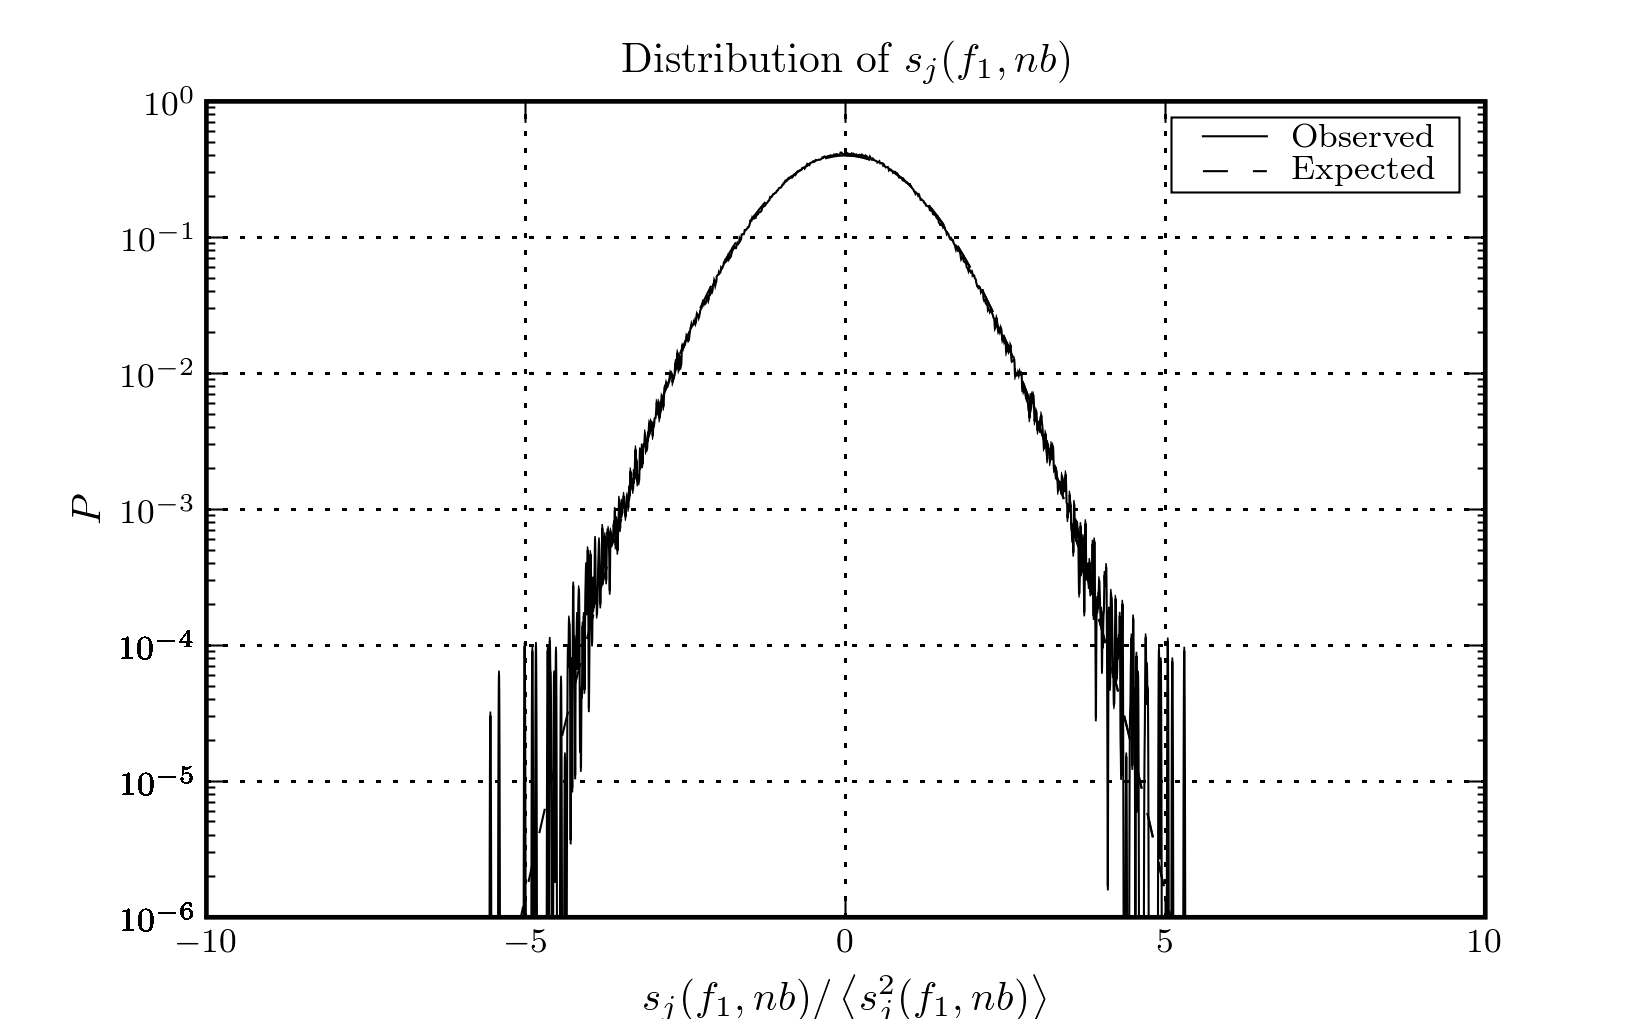
\includegraphics{figures/h_histogram.png}}
\end{center}
\caption{The distribution of samples observed in the approximate unwhitened
time series (of varying bandwidths) normalized to the expected root mean
square value.}
\label{fig:sjhistogram}
\end{figure}

Finally,
\begin{equation}
\sum_{j} h_{j}^{2}(f_{1}, n b) \Delta t
   = \sum_{j} s_{j}^{2}(f_{1}, n b) \Delta t - d \mean{s_{j}^{2}(f_{1}, n
   b)} \Delta t,
\end{equation}
so,
\begin{equation}
h_{\text{rss}}
   = \sqrt{\sum_{j} s_{j}^{2}(f_{1}, n b) \Delta t - d
   \mean{s_{j}^{2}(f_{1}, n b)} \Delta t}.
\end{equation}
A example of the results can be see in Figures \ref{fig:h_rec_vs_inj}.
\begin{figure}
\begin{center}
\resizebox{3.75in}{!}{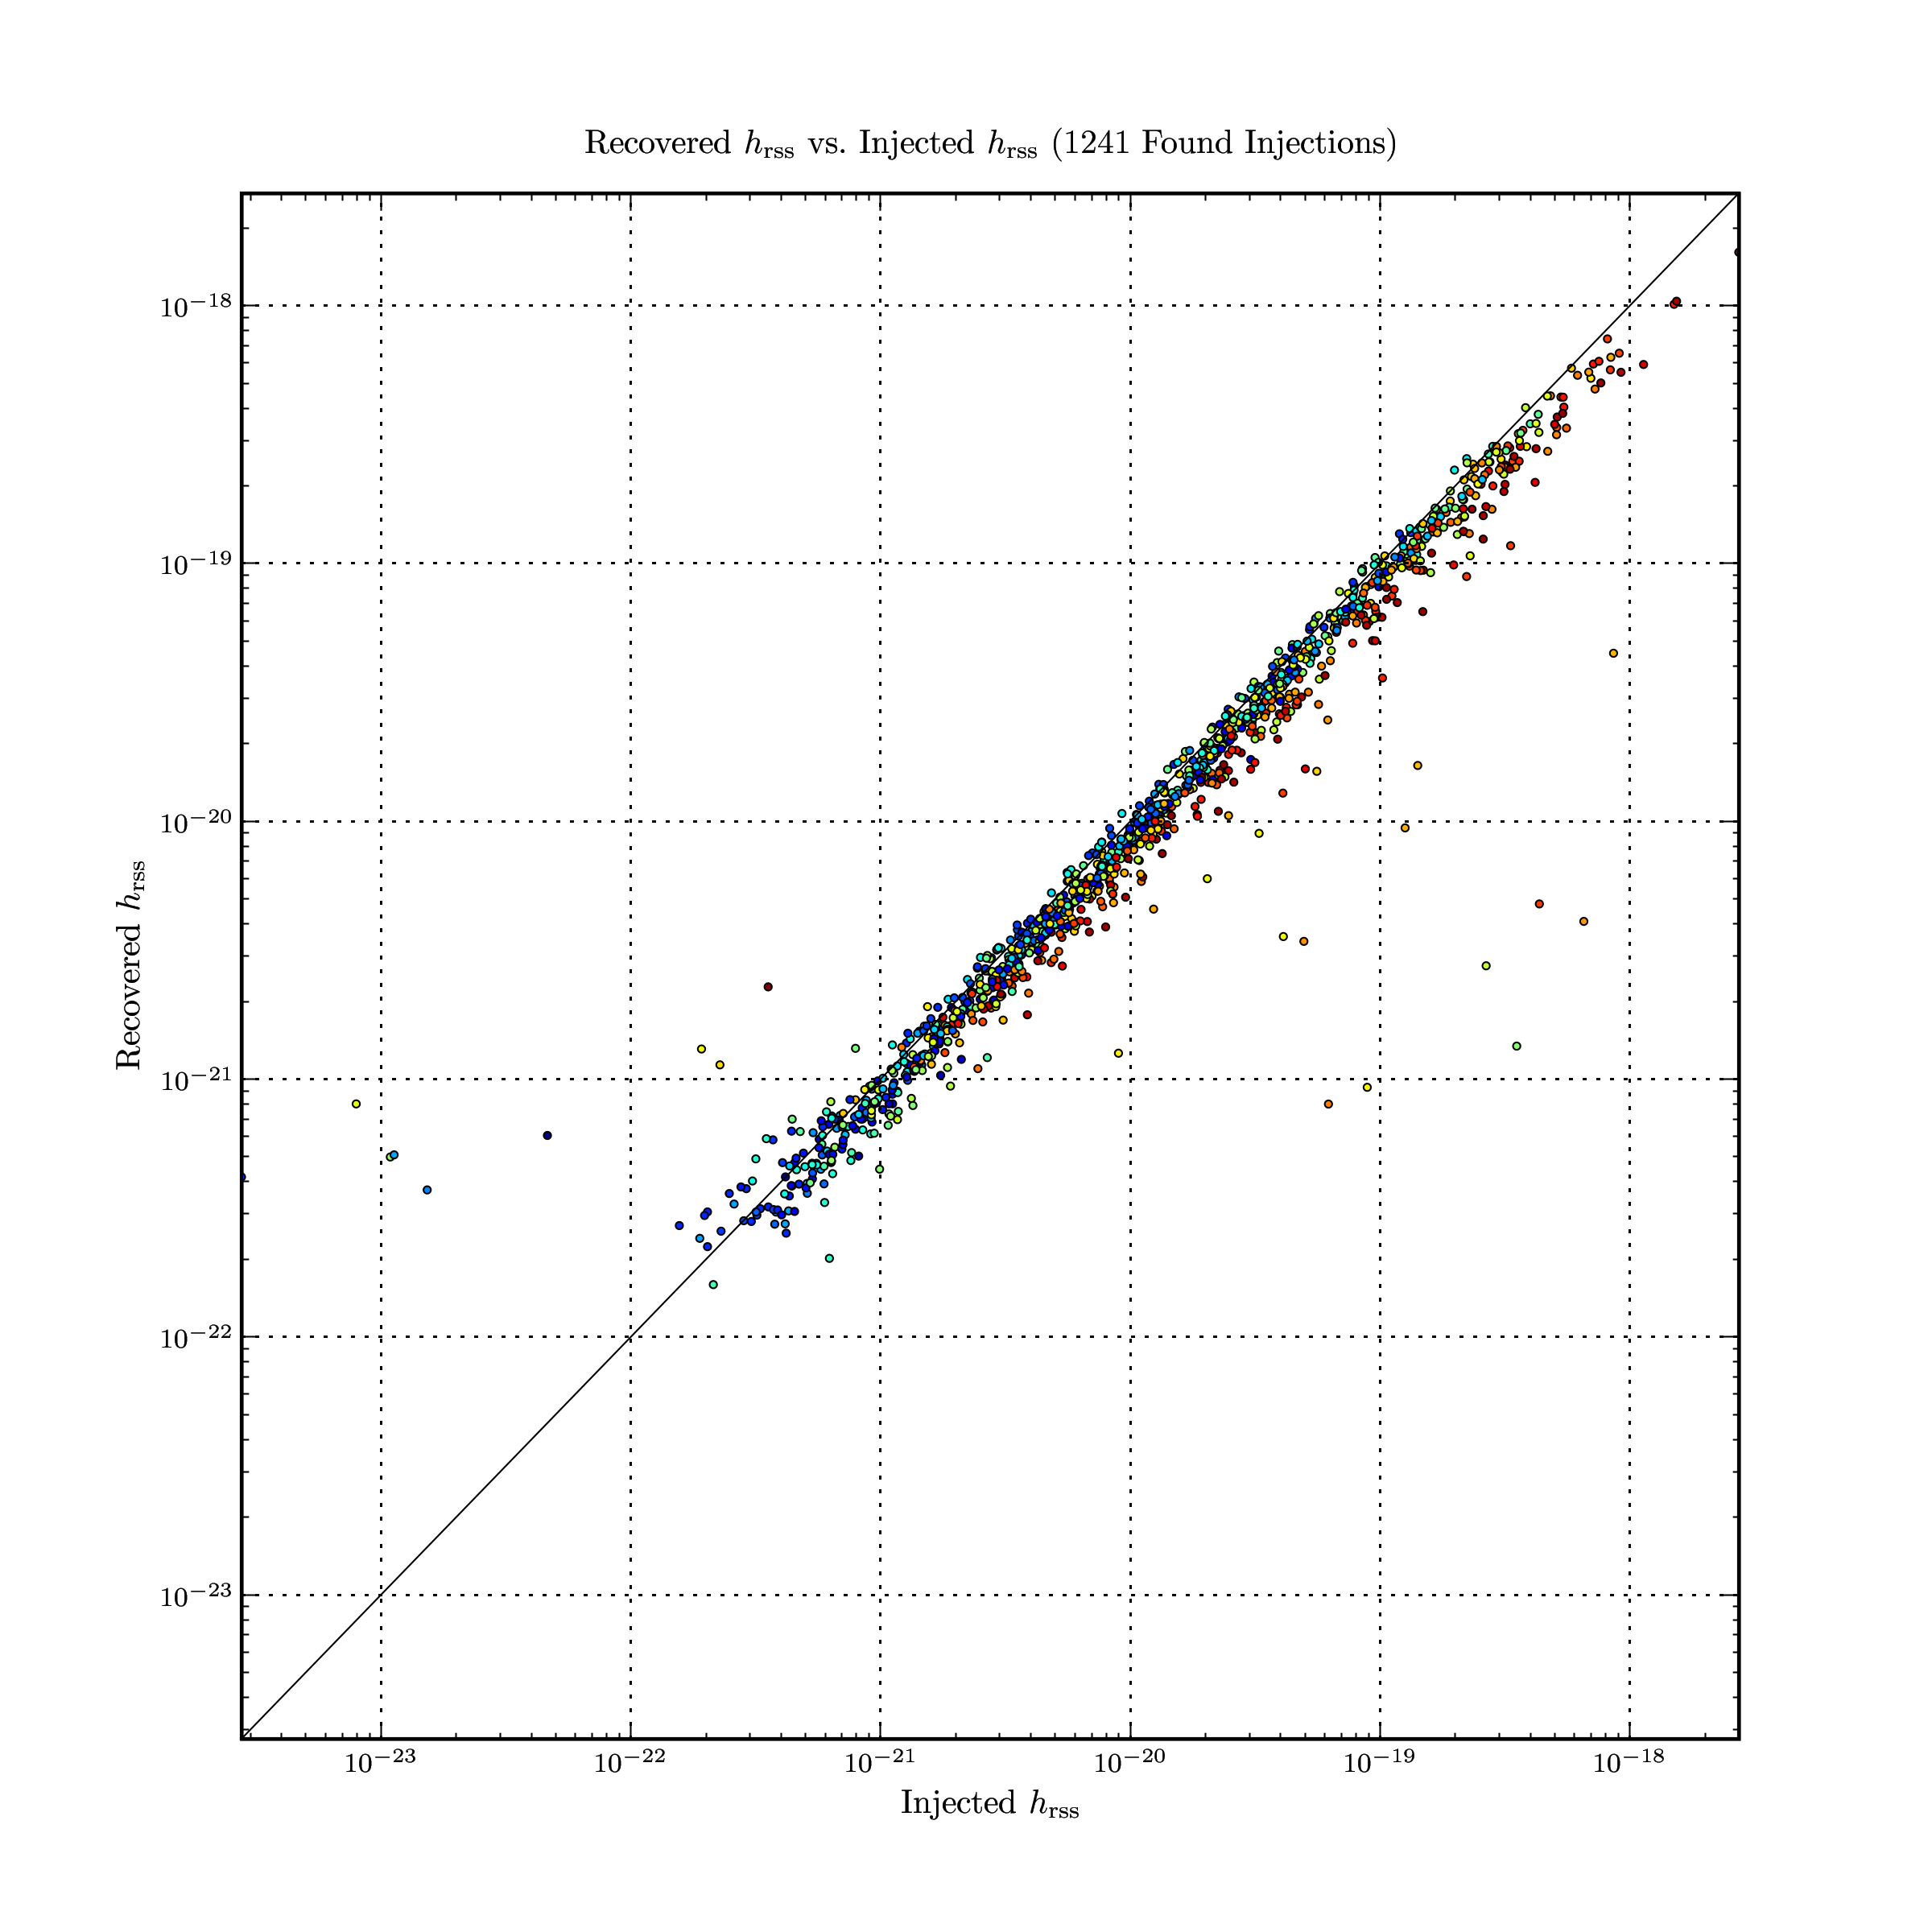
\includegraphics{figures/plotbinj_L1_4.png}}
\resizebox{3.75in}{!}{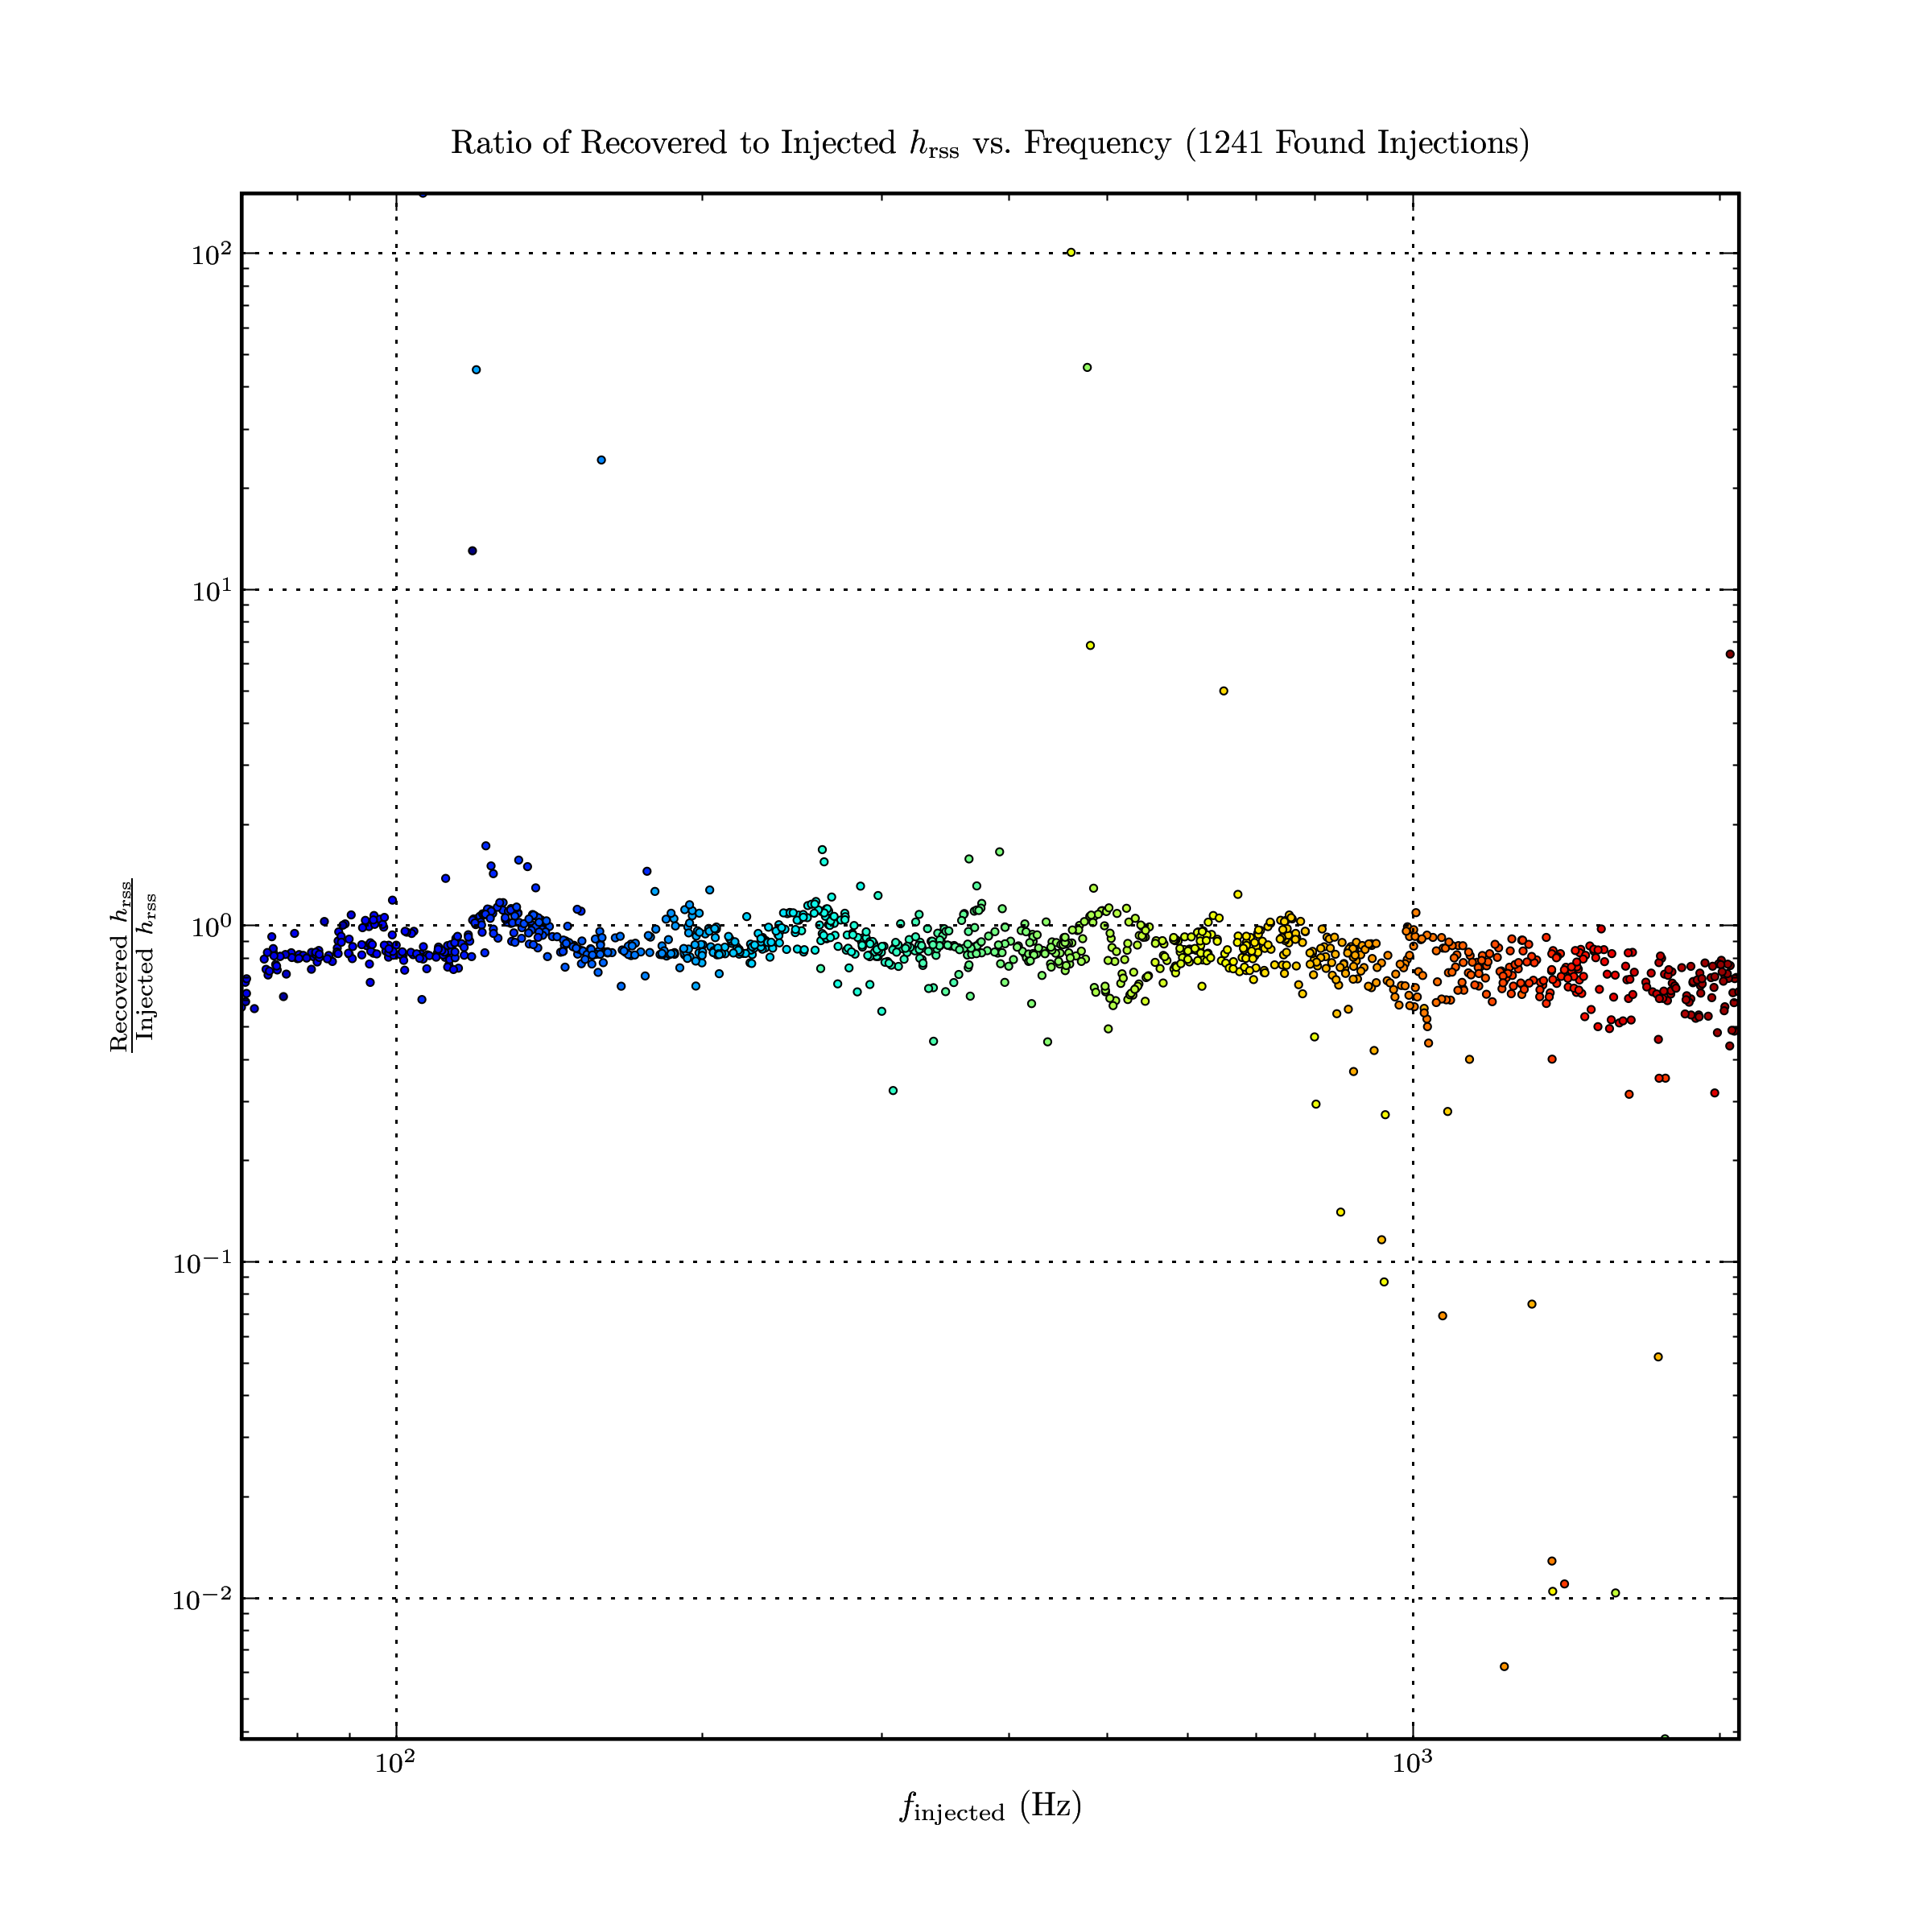
\includegraphics{figures/plotbinj_L1_5.png}}
\end{center}
\caption{Scatter plots of recovered vs.\ injected
\(h_{\text{rss}}^{\text{det}}\) for an all-sky population of \(Q = 8.89\)
sine-Gaussian linearly-polarized waveforms.  In both plots colour indicates
the frequency at which the event was recovered.  The top plot is recovered
vs.\ injected \(h_{\text{rss}}^{\text{det}}\), the bottom plot shows the
recovered-to-injected \(h_{\text{rss}}^{\text{det}}\) ratio vs.\ the
frequency at which the event was recovered.  In both plots, the colour
indicates the centre frequency of the injection.}
\label{fig:h_rec_vs_inj}
\end{figure}

It must be remarked that this procedure can occasionally yield an estimated
\(h_{\text{rss}}\) that is not real-valued.  This happens when the observed
unwhitened energy, \(\sum_{j} s_{j}^{2} \Delta t\), proves to be less than
the expected unwhitened energy, \(d \mean{s_{j}^{2}} \Delta t\).  The
whitened energy is always greater than the expected amount by construction
because we threshold on it, discarding any tiles below some cut-off.
Another way of expressing this is to say that the whitened SNR is always
greater than 1, but the unwhitened SNR need not be.  This should not be
unexpected because the arithmetic by which the frequency-domain data is
turned into a whitened and unwhitened sum-squares weights different
frequency bins differently.  In particular, non-real \(h_{\text{rss}}\)
values are seen more frequency in the vicinity of strong line features such
as the violin modes, where the difference between the whitened and
unwhitened spectra are the greatest.  The search code discards any tiles
whose estimated \(h_{\text{rss}}\) is not real-valued.


\subsubsection{Over-Whitening}


Section \ref{sec:channelfilter} began with the comment that the choice of
channel filter is mostly irrelevant, so long as there is some sense in
which it corresponds to a particular frequency band.  In the derivations
that followed, the approximation was made that only adjacent channel
filters have any appreciable overlap.  A particular choice of channel
filter was described, but other choices are possible.  One improvement that
can be made is to identify lines in the spectral density, and add notches
to the channel filters to remove them.  Often these spectral line features
are the result of noise processes in the instrument or its environment.
For example, suspension wire resonances, harmonics of the
\(\unit{60}{\hertz}\) power line frequency, and optic resonances are all
prominently visible in the spectrum of LIGO interfermeter.  The effect of
adding notches at these frequencies is to cause the search to measure the
energy in the time-frequency tiles preferentially from those frequency
bands less contaminated by these noise sources.

A simple way of deweighting contaminated frequency bands is to divide the
channel filters by some power of the power spectral density,
\begin{equation}
\tilde{\Theta}_{k}'(f_{1}, B)
   \propto P_{k}^{-a} \tilde{\Theta}_{k}(f_{1}, B).
\end{equation}
The modified channel filters are normalized as before.  When \(a =
\frac{1}{2}\), that is the nominal channel filters are divided by the
square root of the power spectral density, the procedure is called ``over
whitening''.  There are, aparently, theoretical reasons to make this
choice.  Over-whitening is found to significantly improve the ability of
the excess power search to reject noise, and so the actual channel filters
used by the search are not only the Hann windows described above but also
contain one inverse power of the square root of the power spectral density.


\subsection{Time Domain Segmentation}


%
% FIXME:  the descriptions here are obsolete
%


The excess power analysis code does not process the input data as a
continuous time series;  rather the time series is split into a sequence of
discrete ``analysis windows'', which are each analyzed individually.  To
account for the possibility of a burst event stradling the boundary between
two analysis windows, successive windows are staggered in such a way that
they overlap one another in time.  In this way, a burst event occuring on
the boundary of one window will (typically) be centred in the next.

Because edge effects at various stages of the analysis can corrupt the
beginning and end of the analysis window, the actual quantity of data
extracted from the input time series to form a window is twice the amount
that is analyzed.  Only results from the central half of the window are
retained, with the first and last quarters of each window being discarded.
The arrangement is shown in the following diagram.
\begin{center}
\begin{picture}(0,0)%
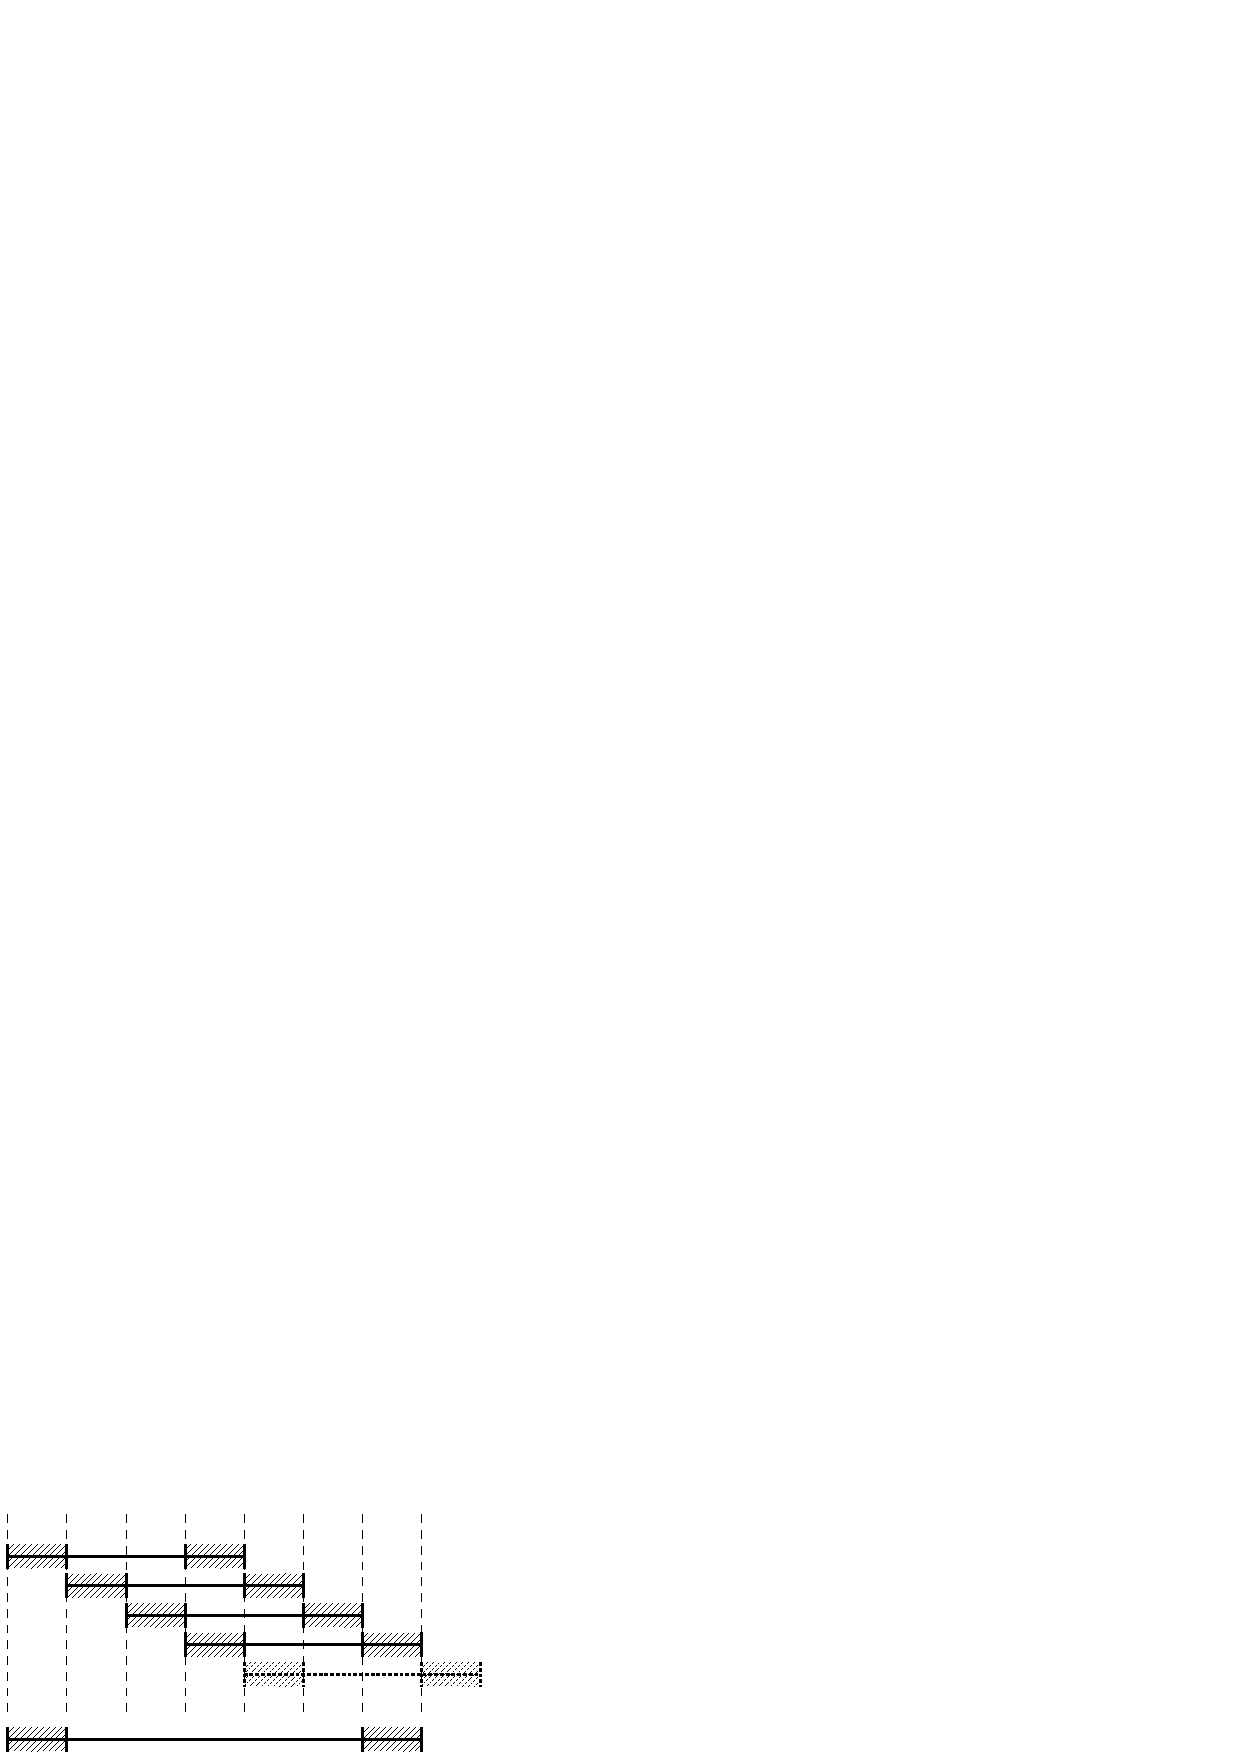
\includegraphics{figures/power/windows.fig.pdf}%
\end{picture}%
\setlength{\unitlength}{4144sp}%
%
\begingroup\makeatletter\ifx\SetFigFont\undefined%
\gdef\SetFigFont#1#2#3#4#5{%
  \reset@font\fontsize{#1}{#2pt}%
  \fontfamily{#3}\fontseries{#4}\fontshape{#5}%
  \selectfont}%
\fi\endgroup%
\begin{picture}(3194,1329)(-21,-253)
\put( 46,929){\makebox(0,0)[lb]{\smash{{\SetFigFont{10}{12.0}{\familydefault}{\mddefault}{\updefault}0}}}}
\put(1846,929){\makebox(0,0)[lb]{\smash{{\SetFigFont{10}{12.0}{\familydefault}{\mddefault}{\updefault}32768}}}}
\put(3151,434){\makebox(0,0)[lb]{\smash{{\SetFigFont{10}{12.0}{\familydefault}{\mddefault}{\updefault}\(\cdots\)}}}}
\end{picture}%

\end{center}
Here we see a discrete time series (represented by the bottom-most
horizontal line) that contains 57344 samples.  It has been divided into a
sequence of four analysis windows, each containing 32768 samples.  A fifth,
greyed-out, analysis window is shown to indicate where the next window in
the sequence would start.  In the analysis of each window, the first and
last 8192 samples (first and last quarter) are discarded as indicated by
the crossed-out sections in each window.  In this particular example, each
window is shifted 8192 samples (also equal to one quarter of the window
length) from the start of the previous window.  This choice of window
length and window shift causes the sections of each window that are
actually searched for events (the sections that are not crossed out) to
overlap their neighbours by half of their own width.  This is the typical
mode of operation for the search code.  Notice that the first and last
quarter window length of the complete time series (the cross-out sections
in the bottom line) are \emph{not} analyzed, as they are discarded from the
only analysis windows in which they appear.

The excess power code whitens the input time series using an estimate of
the instrument's noise power spectral density (PSD).  The estimated noise
PSD is computed by averaging the PSDs from a number of successive analysis
windows.  The noise PSD is not estimated by averaging over the entire time
series in order to allow the code to track the (possibly) changing
character of the instrument's noise.  For convenience, the user is
permitted to enter the number of samples that should be used to estimate
the PSD.  The number of samples entered should correspond to the time for
which the instrument's noise can be approximated as stationary for the
purpose of the excess power analysis.  Since, however, the actual
estimation procedure involves averaging over an integer number of analysis
windows, it is necessary for the number of samples selected to correspond
to the boundary of an analysis window.  For convenience,
\prog{lalapps\_power} will automatically round the value entered down to
the nearest analysis window boundary.

The LAL function \function{EPSearch()} performs the parts of the analysis
described above.  It is given a time series that it divides into analysis
windows, which it uses to estimate the noise PSD.  Using the estimated
noise PSD, it whitens each analysis window and then searches them for burst
events.  Only the analysis windows within the data used to estimate the
noise PSD are whitened using that estimate.  Once those windows have been
searched for burst events, \function{EPSearch()} returns to the calling
procedure which then extracts a new time series from the input data and the
process repeats.  The parameter provided via the command line option
\option{--psd-average-points} sets the length of the time series that is
passed to \function{EPSearch()}.

As successive time series are passed to \function{EPSearch()}, in order for
the first analysis window to correctly overlap the last window from the
previous time series --- i.e.\ to ensure the same overlap between analysis
windows in neighbouring time series as exists between neighbouring windows
within a series --- it is necessary for the latter time series to begin
$(\mbox{\parm{window length}} - \mbox{\parm{window shift}})$ samples before
the end of the former series.  The arrangement is shown in the following
figure.
\begin{center}
\begin{picture}(0,0)%
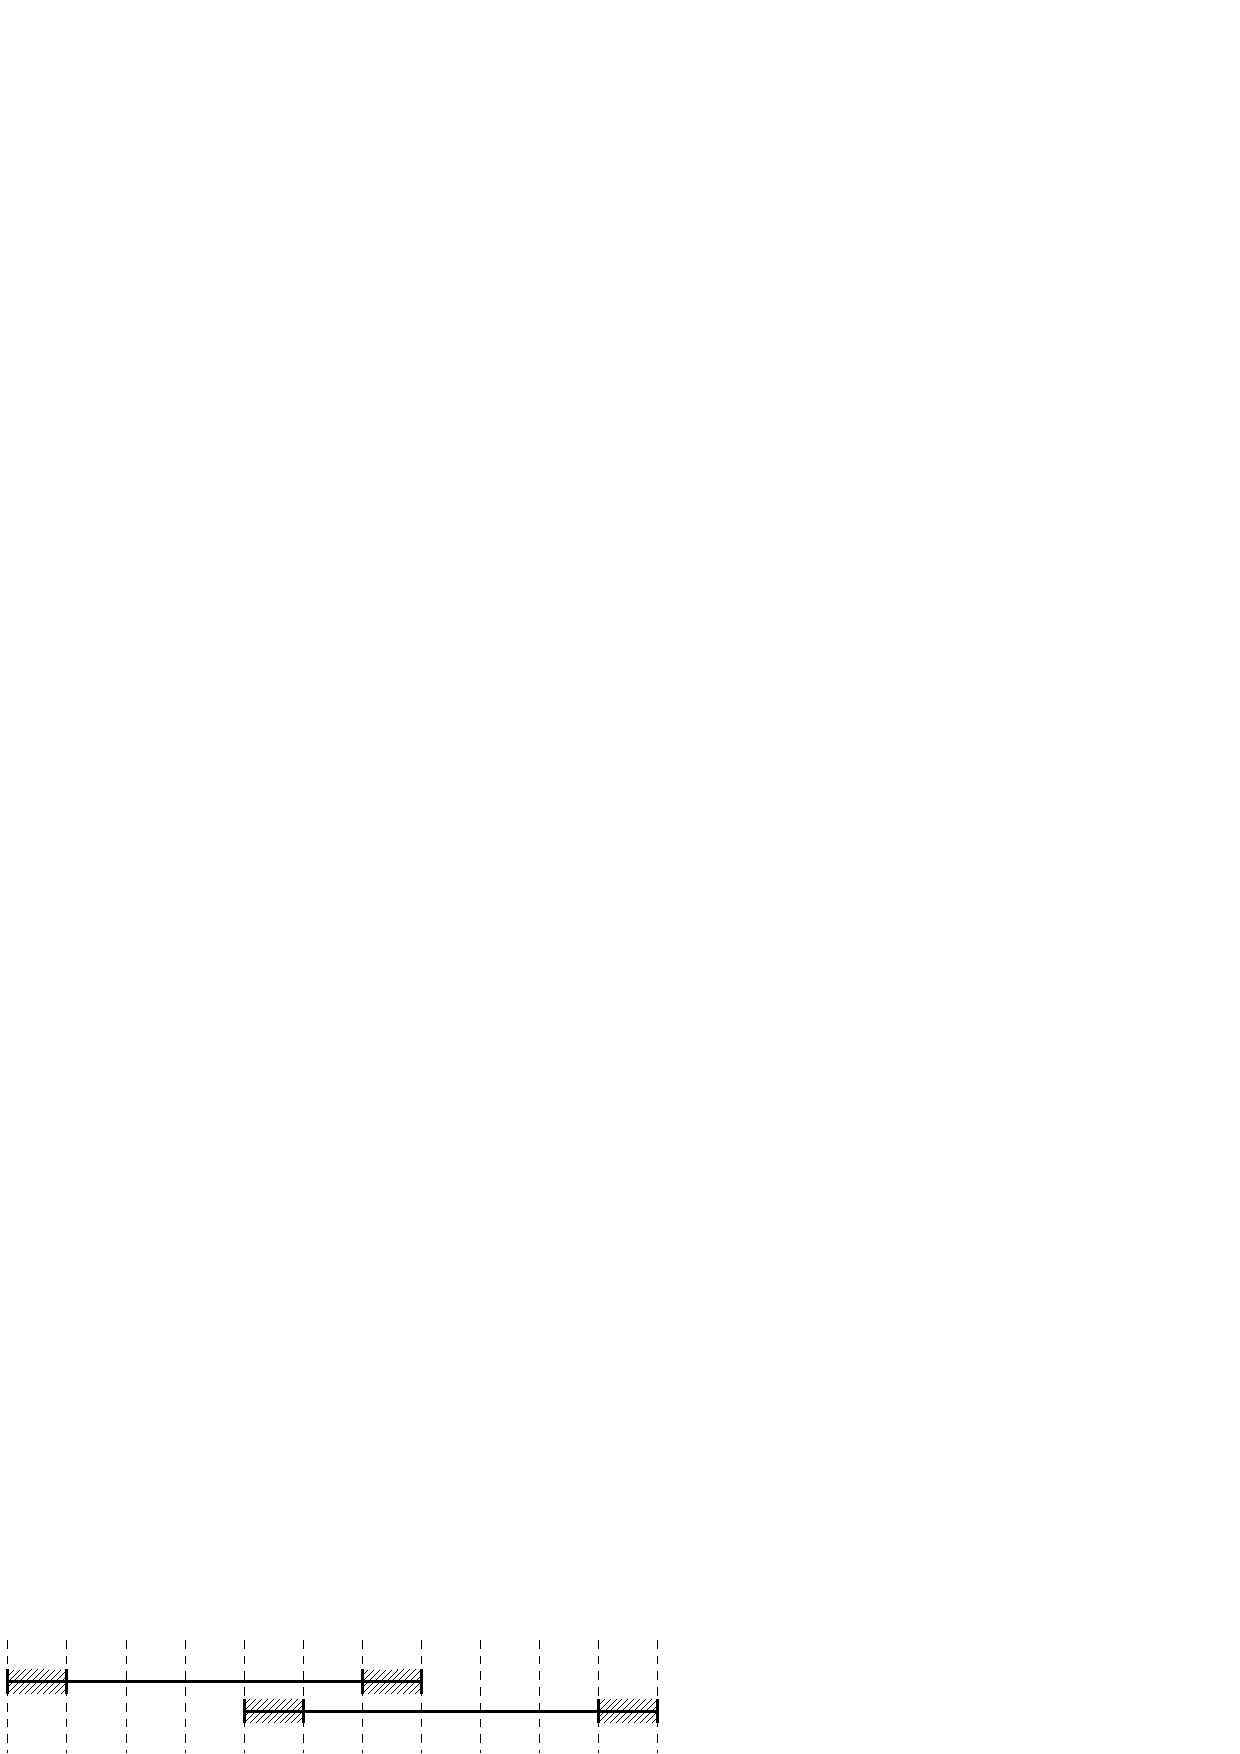
\includegraphics{figures/power/psds.fig.pdf}%
\end{picture}%
\setlength{\unitlength}{4144sp}%
%
\begingroup\makeatletter\ifx\SetFigFont\undefined%
\gdef\SetFigFont#1#2#3#4#5{%
  \reset@font\fontsize{#1}{#2pt}%
  \fontfamily{#3}\fontseries{#4}\fontshape{#5}%
  \selectfont}%
\fi\endgroup%
\begin{picture}(5364,1032)(-59,197)
\put(-44,1109){\makebox(0,0)[lb]{\smash{{\SetFigFont{10}{12.0}{\familydefault}{\mddefault}{\updefault}0}}}}
\put(1756,1109){\makebox(0,0)[lb]{\smash{{\SetFigFont{10}{12.0}{\familydefault}{\mddefault}{\updefault}32768}}}}
\put(3106,1109){\makebox(0,0)[lb]{\smash{{\SetFigFont{10}{12.0}{\familydefault}{\mddefault}{\updefault}57344}}}}
\put(4906,1109){\makebox(0,0)[lb]{\smash{{\SetFigFont{10}{12.0}{\familydefault}{\mddefault}{\updefault}90112}}}}
\end{picture}%

\end{center}
Here we see two of the time series from the first diagram above, each of
which is to be passed to \function{EPSearch()} for analysis.  To see why
the overlap between these two time series must be chosen as it is, refer to
the first diagram above to see where the greyed-out fifth analysis window
was to be placed.  That is where the first analysis window in the second
time series here will be placed.

Prior to looping over the data one noise PSD estimation length at a time,
the data is passed through a conditioning filter.  To account for edge
effects in the filter, an amount of data set by the command line option
\option{--filter-corruption} is dropped from the analysis at both the
begining and end of the time series.  The arrangement is shown in the
following diagram.
\begin{center}
\begin{picture}(0,0)%
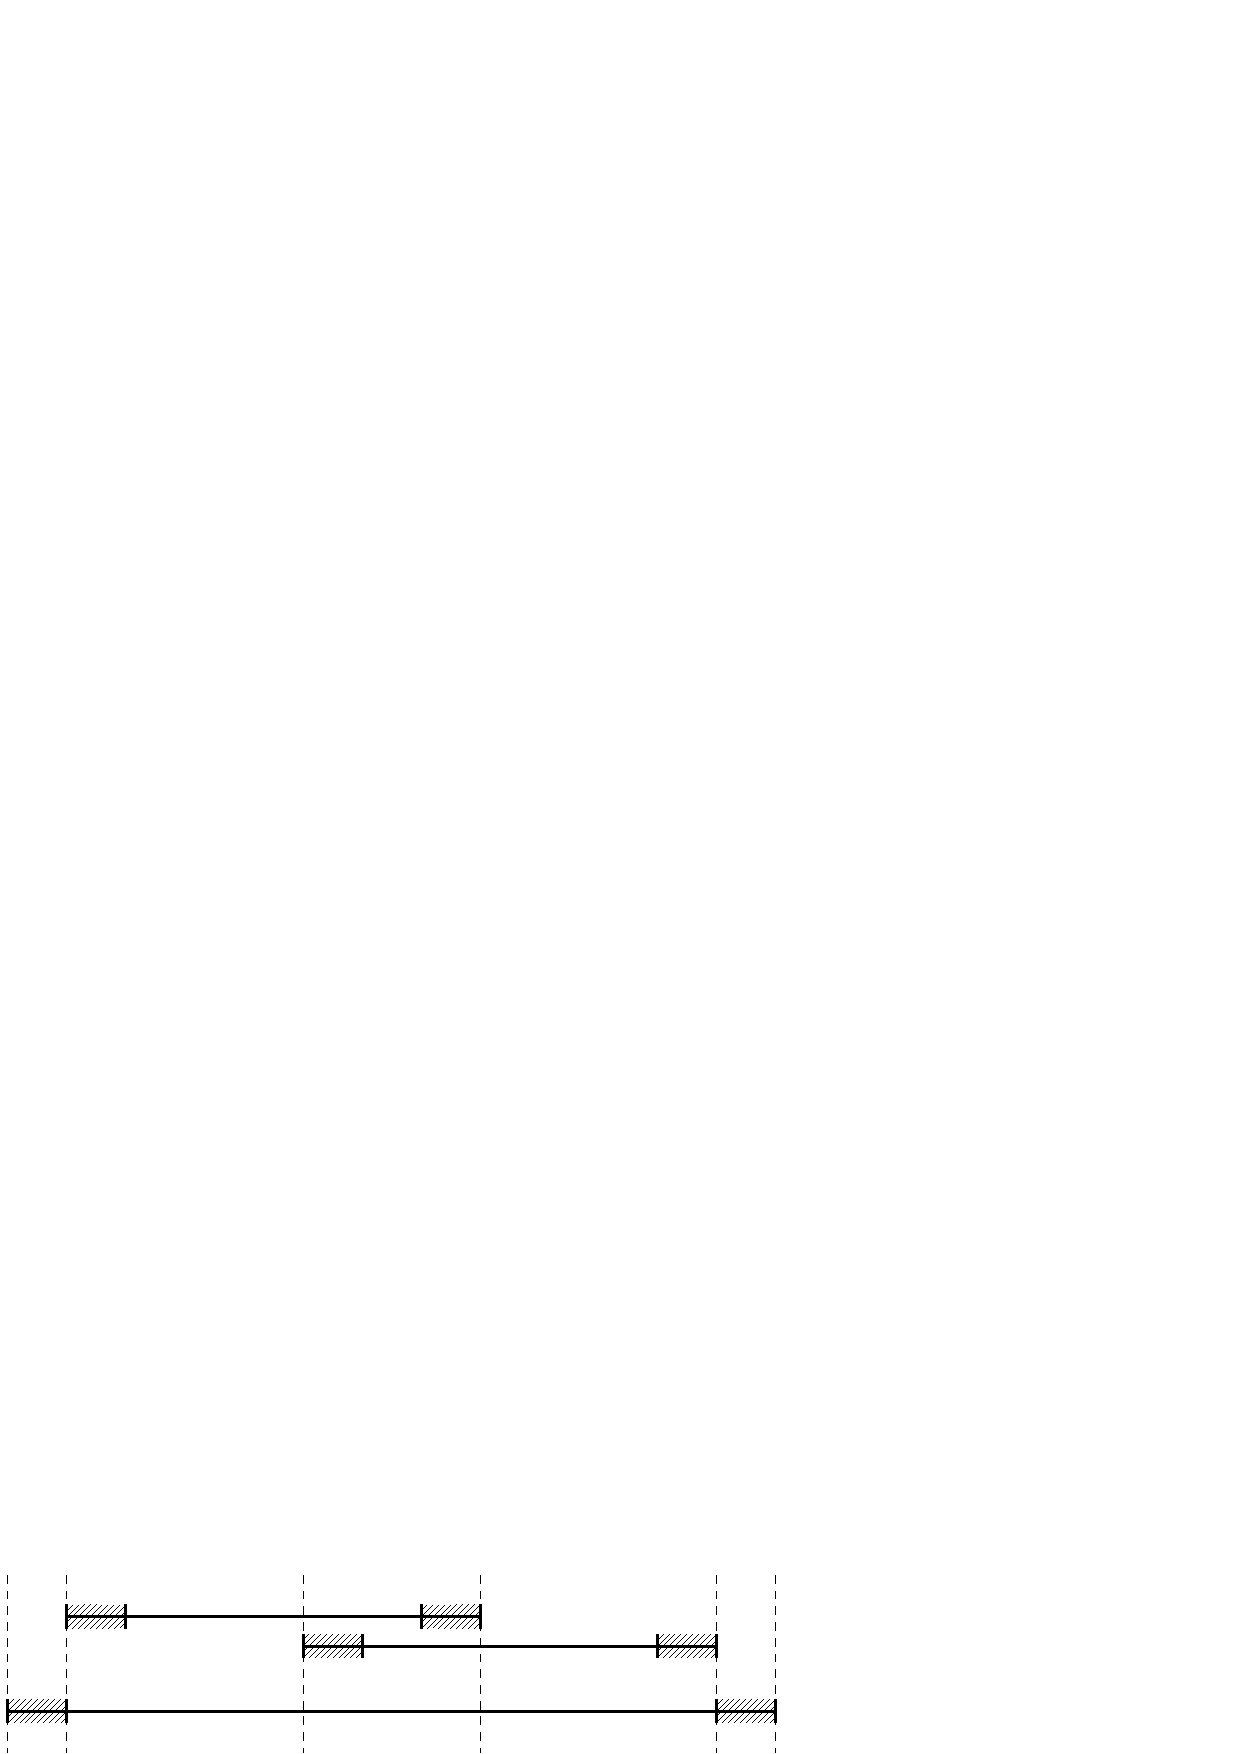
\includegraphics{figures/conditioning.fig.pdf}%
\end{picture}%
\setlength{\unitlength}{4144sp}%
%
\begingroup\makeatletter\ifx\SetFigFont\undefined%
\gdef\SetFigFont#1#2#3#4#5{%
  \reset@font\fontsize{#1}{#2pt}%
  \fontfamily{#3}\fontseries{#4}\fontshape{#5}%
  \selectfont}%
\fi\endgroup%
\begin{picture}(6341,1527)(-509,-298)
\put(-494,1109){\makebox(0,0)[lb]{\smash{{\SetFigFont{10}{12.0}{\familydefault}{\mddefault}{\updefault}0}}}}
\put(-44,1109){\makebox(0,0)[lb]{\smash{{\SetFigFont{10}{12.0}{\familydefault}{\mddefault}{\updefault}8192}}}}
\put(1756,1109){\makebox(0,0)[lb]{\smash{{\SetFigFont{10}{12.0}{\familydefault}{\mddefault}{\updefault}40960}}}}
\put(3106,1109){\makebox(0,0)[lb]{\smash{{\SetFigFont{10}{12.0}{\familydefault}{\mddefault}{\updefault}65536}}}}
\put(4906,1109){\makebox(0,0)[lb]{\smash{{\SetFigFont{10}{12.0}{\familydefault}{\mddefault}{\updefault}98304}}}}
\put(5356,1109){\makebox(0,0)[lb]{\smash{{\SetFigFont{10}{12.0}{\familydefault}{\mddefault}{\updefault}106496}}}}
\end{picture}%

\end{center}
The bottom-most line in this diagram represents the time series as read
into memory from disk.  In this example we have read 106496 samples into
memory, and after passing it through the conditioning filter 8192 samples
are dropped from the beginning and end of the series.  The remaining data
is then passed to \function{EPSearch()} 57344 samples at a time --- just as
was done in the earlier examples --- with appropriate overlaps.  In this
example, it happens that an integer number of overlaping noise PSD
intervals fits into the data that survives the conditioning.  In general
this will not be the case.  If the last noise PSD interval would extend
beyond the end of the time series, it is moved to an earlier time so that
its end is aligned with the end of the available data.

If more data needs to be analyzed than will fit in RAM at one time, we must
read it into memory and analyze it in pieces.  In doing this, we again want
the analysis windows in neighbouring read cycles to overlap one another in
the same manner that neighbouring analysis windows within a single noise
PSD interval overlap one another.  This will be assured if, in the diagram
above, the start of the next data to be read from disk is arranged so that
the first noise PSD interval to be analyzed within it starts at the correct
location relative to the last PSD interval analyzed from the previous read
cycle.  Consideration of the diagram above reveals that in order to meet
this condition, the next data to be read into memory should start $(2
\times \mbox{\parm{filter corruption}} + \mbox{\parm{window length}} -
\mbox{\parm{window shift}})$ samples prior to the end of the previous data
to have been read.


\subsection{Band and Time Limited White-Noise Burst Injections}


% FIXME:  I change notation here:  now \Delta t and \Delta f are the
% duration and bandwidth of the injection respectively instead of the
% sample resolutions in the time and frequency series.


\subsubsection{Overview}


The excess power algorithm is the optimum detection strategy for waveforms
whose energy is confined to a given pass band and time interval, but where
nothing else is known about the waveform.  For characterizing the pipeline,
it is necessary to produce such waveforms:  waveforms of unknown structure
except for having their energy confined to a chosen pass band and time
interval.  We can construct such waveforms by applying to stationary white
Gaussian noise a time-domain window function and then a frequency domain
window function so as to retain energy only within the desired time
interval and frequency band.  We shall refer to the result of this
procedure a band- and time-limited white-noise burst waveform (BTLWNB).


\subsubsection{Construction}


The construction of a BTLWNB waveform with duration \(\Delta t\) and
bandwidth \(\Delta f\) centred on \(f_{0}\) begins by populating a time
series with independent Gaussian random numbers.  The origin of the time
co-ordinate corresponds to the middle sample in the time series.  We apply
an initial time-limiting window function to the time series by multiplying
the time series with a Gaussian window function
\begin{equation}
w_{1}(t)
   \propto \ee^{-\frac{1}{2} t^{2} / \sigma_{t}^{2}},
\end{equation}
where \(\sigma_{t}\) sets the duration of the window.  The windowed time
series is then Fourier transformed and a second Gaussian window applied in
the frequency domain
\begin{equation}
\tilde{w}_{2}(f)
   \propto \ee^{-\frac{1}{2} (f - f_{0})^{2} / \sigma_{f}^{2}},
\end{equation}
where \(\sigma_{f} = \frac{1}{2} \Delta f\).

Since the inital time series is real-valued, the negative frequency
components of the Fourier transform are the complex conjugates of the
positive frequency components and need not be stored.  The frequency-domain
filter is real-valued (phase preserving), and so when the positive
frequency components are the only ones being stored applying the window
function to them alone achieves the correct result.

The multiplication of the frequency domain data by the window function is
equivalent to convolving the time domain data with the Fourier transform of
the window.  Since the Fourier transform of the frequency window is not a
\(\delta\) function, the application of the band-limiting window has the
effect of spreading the signal in the time domain, i.e.\ increasing its
duration.  We can compensate for this by choosing an appropriate value for
\(\sigma_{t}\) so that the waveform has the correct duration \emph{after}
application of the frequency domain window.  The inverse Fourier transform
of \(\tilde{w}_{2}(f)\) is
\begin{equation}
w_{2}(t)
   \propto \ee^{-2 \pi^{2} \sigma_{f}^{2} t^{2}}.
\end{equation}
The result of convolving two Gaussians with one another is another
Gaussian, so the effective time-domain window is
\begin{equation}
w(t)
   = w_{1}(t) \otimes w_{2}(t)
   \propto \ee^{-\frac{1}{2} t^{2} / \sigma^{2}},
\end{equation}
where
\begin{equation}
\sigma^{2}
   = \sigma_{t}^{2} + \frac{1}{4 \pi^{2} \sigma_{f}^{2}}
   = \sigma_{t}^{2} + \frac{1}{\pi^{2} \Delta f^{2}}
\end{equation}
We wish this Gaussian's width to be \(\sigma = \frac{1}{2} \Delta t\),
therefore
\begin{equation}
\sigma_{t}
   = \sqrt{\frac{1}{4} \Delta t^{2} - \frac{1}{\pi^{2} \Delta f^{2}}}.
\end{equation}
Note that \(\sigma_{t}\) is only real-valued when
\begin{equation}
\Delta t \Delta f
   \geq \frac{2}{\pi}.
\end{equation}

After application of the frequency domain window the data is inverse
transformed to the time domain for injection into the strain data.


\subsubsection{Details}


The algorithm described here yields a single time series containing a band-
and time-limited white noise burst waveform.  The injection generator
produces both \(h_{+}\) and \(h_{\times}\) waveforms.  These are
independent waveforms constructed by simply applying the time series
construction algorithm twice.  The injection code uses a time series whose
length is \(10 \Delta t\) rounded to the nearest odd integer,
\begin{equation}
L
   = 2 \left\lfloor \frac{1}{2} \frac{10 \Delta t}{\delta t} \right\rfloor
   + 1
\end{equation}
where \(\delta t\) is the sample period of the time series.  The middle
sample is \(t = 0\), so the first and last samples are at \(t = \pm \delta
t (L - 1) / 2\).  The time-domain Gaussian window is constructed with a
call to \texttt{XLALCreateGaussREAL8Window()} with a shape parameter of
\begin{equation}
\beta
   = \frac{(L - 1) \delta t / 2}{\sigma_{t}}.
\end{equation}
The numerator transforms the normalized co-ordinate \(y \in [-1, +1]\) in
the definition of the window function to \(t\).\footnote{See the LAL
documentation for more information.  Sample index 0 is \(y = -1\), sample
index \(L - 1\) is \(y = +1\), so there are \((L - 1) / 2\) sample indexes
per unit of \(y\).}.

The time series is transformed to the frequency domain with a call to
\texttt{XLALREAL8TimeFreqFFT()}, which populates the metadata of the output
frequency series with the appropriate values.  There are \((L + 1) / 2\)
complex-valued frequency components with a bin spacing of \(\delta f = (L
\delta t)^{-1}\).  The first bin's frequency is \(\unit{0}{\hertz}\), and
altogether they span a frequency of \(f = \delta f (L + 1) / 2\).  The
frequency domain Gaussian window is constructed with a call to
\texttt{XLALCreateGaussREAL8Window()} requesting a window with a length
twice that of the frequency series, and a shape parameter of
\begin{equation}
\beta
   = \frac{L \delta f / 2}{\sigma_{f}}.
\end{equation}
The window is created with the peak centered in the vector, so we will need
to shift the samples to place the peak at the correct frequency.
Requesting a window twice as long as the frequency series ensures that we
will still have a complete set of samples after they are shifted.  The
numerator in the shape parameter converts the normalized co-ordinate \(y
\in [-1, +1]\) in the definition of the window function to
frequency.\footnote{See the LAL documentation for more information.  The
window is twice the length of the frequency series, sample index 0 is \(y =
-1\), sample index \(L + 1\) is \(y = +1\), so there are \(L / 2\) sample
indexes per unit of \(y\).}  The frequency-domain window's samples are
shifted with a call to \texttt{XLALResizeREAL8Sequence()}, which is used to
extract \((L + 1) / 2\) samples starting at index \(\lfloor (L + 1) / 2 -
f_{0} / \delta f \rfloor\).

Following application of the frequency-domain window, the injection is
transformed back to the time domain with a call to
\texttt{XLALREAL8FreqTimeFFT()}.  If \(\tilde{h}_{k}\) are the complex
values in the frequency bins, the output time series is
\begin{equation}
h_{j}
   = \delta f \sum_{k = 0}^{L - 1} \tilde{h}_{k} \ee^{2 \pi \aye j k / L}
   = \delta f \sum_{k = 0}^{L - 1} \tilde{h}_{k} \ee^{2 \pi \aye t k / (L
   \delta t)},
\end{equation}
where \(t = j \delta t\).  Differentiating with respect to \(t\),
\begin{equation}
\dot{h}_{j}
   = \delta f \sum_{k = 0}^{L - 1} \left( \frac{2 \pi \aye k}{L \delta t}
   \right) \tilde{h}_{k} \ee^{2 \pi \aye j k / L},
\end{equation}
and so
\begin{align}
\sum_{j = 0}^{L - 1} \dot{h}_{j}^{2} \delta t
   & = \delta f^{2} \delta t \sum_{k = 0}^{L - 1} \sum_{k' = 0}^{L - 1}
   \left( \frac{4 \pi^{2} k k'}{L^{2} \delta t^{2}} \right) \tilde{h}_{k}
   \conj{\tilde{h}_{k'}} \sum_{j = 0}^{L - 1} \ee^{2 \pi \aye j (k - k') /
   L}
   \\
   & = \delta f^{2} L \delta t \sum_{k = 0}^{L - 1} \left( \frac{4 \pi^{2}
   k^{2}}{L^{2} \delta t^{2}} \right) \magnitude{\tilde{h}_{k}}^{2}
   \\
   & = 4 \pi^{2} \delta f \sum_{k = 0}^{L - 1} (k \delta f)^{2}
   \magnitude{\tilde{h}_{k}}^{2}.
\end{align}
This relationship is used to normalize the injection time series.  The
expression on the left hand side is \(\int \dot{h}^{2} \diff t\).  For both
polarizations the right hand side is computed in the frequency domain
following application of the Gaussian window, and the amplitudes of the
frequency components scaled prior to conversion to the time domain so that
\(\int (\dot{h}_{+}^{2} + \dot{h}_{\times}^{2}) \diff t\) has the desired
value.

To ensure no discontinuities in the strain time series when the injection
is added to it, a final Tukey window is applied to the injection in the
time domain.  The Tukey window is constructed with a call to
\texttt{XLALCreateTukeyREAL8Window()} with a shape parameter of \(\beta =
0.5\) so that the tapers span a total of 50\% of the injection time series.
Because the Tukey window is flat with unit amplitude in the middle, it has
no effect on the injection time series where the bulk of the energy is
concentrated, and the large tapers ensure the Tukey window induces
negligble spread of the injection in the frequency domain.  Because the
injection is normalized in the frequency domain prior to transformation to
the time domain, the application of the Tukey window does bias the
normalization slightly by reducing the total energy in the injection,
however the Tukey window's tapers start several \(\sigma_{t}\) away from
the injection's peak and so this effect is negligble.

In order that the waveforms be reproducable so that an analysis can be
repeated, or the waveforms constructed multiple times for injection into
the strain data from more than one instrument, it is necessary to specify
how the initial time series of independent Gaussian random numbers is to be
constructed.  This is done by specifying the seed to be used with the
random number generator.  The random number generator is not specified, so
the same seed may produce different injections with different versions of
the code, but a seed and CVS tag combination should be guaranteed to
produce the same injection.  Note also that changing the length of the
injection time series changes the number of random numbers used to
construct it, so the injection waveform also depends on the time series'
sample rate.  One has to be careful when constructing injection waveforms
for instruments with different sample rates (e.g., LIGO and VIRGO), that
the injection is constructed at some high common sample rate and then down
sampled afterwards for each instrument as needed.

An example of the output of this algorithm is shown in Figure \ref{fig5}
\begin{figure}
\begin{center}
\resizebox{.45\linewidth}{!}{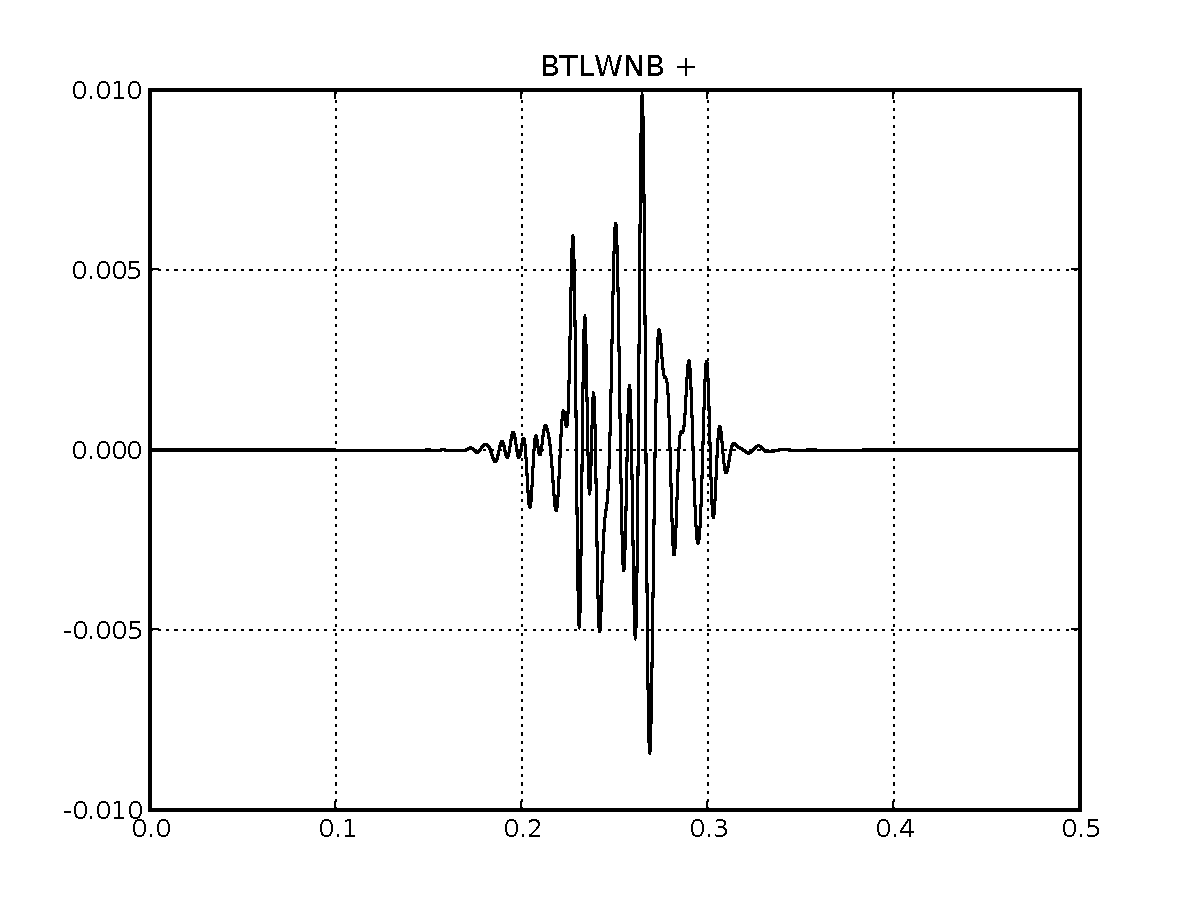
\includegraphics{figures/btlwnb_example_+.pdf}}%
\resizebox{.45\linewidth}{!}{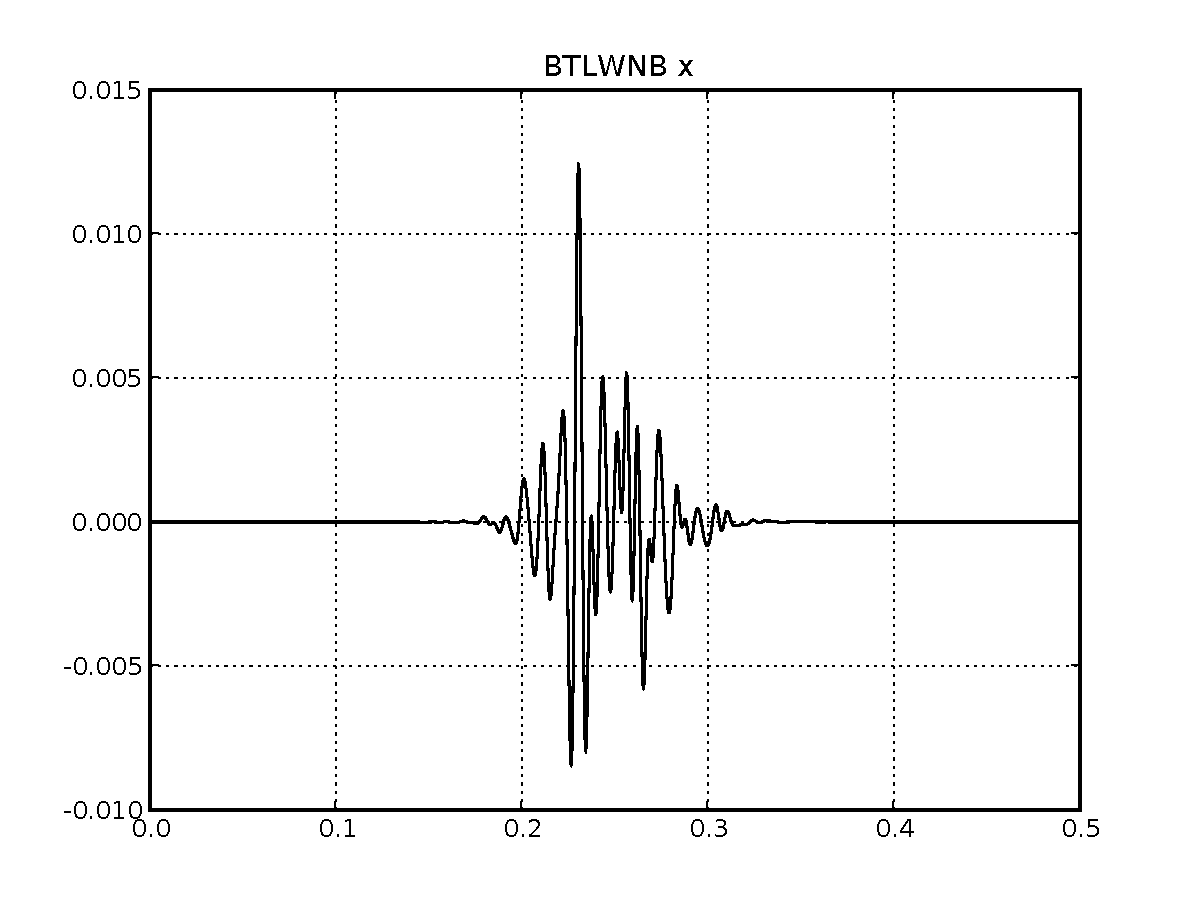
\includegraphics{figures/btlwnb_example_x.pdf}}
\end{center}
\caption{Example of the \(+\) and \(\times\) polarizations of a band- and
time-limited white-noise burst injection waveform.  The horizontal axis is
time in seconds, the vertical axis is strain, and the plots show the full
extent of the time series produced by the injection generator.  The
waveform's paraters were \(\Delta t = \unit{0.05}{\milli\second}\),
\(\Delta f = 8 \frac{2}{\pi} / \Delta t\) (16 degrees of freedom per
polarization), and \(f_{0} = \unit{100}{\hertz}\).  The amplitude was
normalized so that \(\int (\dot{h}_{+}^{2} + \dot{h}_{\times}^{2}) \diff t
= 1\).}
\label{fig5}
\end{figure}


\subsubsection{Normalization}


The local gravitational wave energy flux in the two independent
polarizations, \(h_{+}(t)\) and \(h_{\times}(t)\), is
\begin{equation}
\frac{\diff E}{\diff A \diff t}
   = \frac{1}{16 \pi} \frac{c^{3}}{G} \left( \dot{h}_{+}^{2} +
   \dot{h}_{\times}^{2} \right).
\end{equation}
For a source at non-cosmological distances (distances small enough that for
spheres of that radius \(A = 4 \pi r^{2}\)), the equivalent isotropic
radiated energy in a gravitational wave for a source at a distance \(r\) is
\begin{equation}
E
   = \frac{c^{3}}{4 G} r^{2} \int \left( \dot{h}_{+}^{2}(t) +
   \dot{h}_{\times}^{2}(t) \right) \diff t.
\end{equation}


\section{Program \prog{lalapps\_binj}}
\label{program:lalapps-binj}


\begin{entry}
\item[Name]
\prog{lalapps\_binj} --- produces burst injection data files.

\item[Synopsis]
\prog{lalapps\_binj} \newline \hspace*{0.5in}
[\option{--help}] \newline \hspace*{0.5in}
\option{--gps-start-time}~\parm{tstart} \newline \hspace*{0.5in}
\option{--gps-end-time}~\parm{tend} \newline \hspace*{0.5in}
[\option{--time-step}~\parm{tstep}] \newline \hspace*{0.5in}
[\option{--seed}~\parm{seed}] \newline \hspace*{0.5in}
[\option{--waveform}~\parm{wave}] \newline \hspace*{0.5in}
[\option{--population}~\parm{name}] \newline \hspace*{0.5in}
[\option{--freq-dist}~\parm{name}] \newline \hspace*{0.5in}
[\option{--flow}~\parm{flow}] \newline \hspace*{0.5in}
[\option{--fhigh}~\parm{fhigh}] \newline \hspace*{0.5in}
[\option{--deltaf}~\parm{deltaf}] \newline \hspace*{0.5in}
[\option{--quality}~\parm{quality}] \newline \hspace*{0.5in}
[\option{--tau}~\parm{tau}] \newline \hspace*{0.5in}
[\option{--strain-dist}~\parm{name}] \newline \hspace*{0.5in}
[\option{--strain-scale-min}~\parm{value}] \newline \hspace*{0.5in}
[\option{--strain-scale-max}~\parm{value}] \newline \hspace*{0.5in}
[\option{--max-distance}~\parm{max-distance}] \newline \hspace*{0.5in}
[\option{--min-distance}~\parm{min-distance}] \newline \hspace*{0.5in}
[\option{--simwaveform-duration}~\parm{simwaveform-duration}] \newline \hspace*{0.5in}
[\option{--simwaveform-min-number}~\parm{simwaveform-min-number}] \newline \hspace*{0.5in}
[\option{--simwaveform-max-number}~\parm{simwaveform-max-number}] \newline \hspace*{0.5in}
[\option{--usertag}~\parm{tag}]

\item[Description] 
\prog{lalapps\_binj} generates a number of burst parameters suitable for
using in a Monte Carlo injection to test the efficiency of a burst search.
The various parameters (detailed below) are specified on the command line
or can be randomly chosen in a manner appropriate for an burst upper limit
search.

\prog{lalapps\_binj} produces an injection set following one of two sky
disitributions:  a set of injections from point sources
uniformly-distributed over the sky with uniformly-distributed linear
polarizations, or a set of injections located directly above each
observatory with optimally-oriented linear polarizations.  Which set is
produced is selected by the \option{--population} option.

Injections are produced with various strains, and one of several strain
distributions can be selected with the \option{--strain-dist} parameter.
Some strain distributions require a ``min'' and or a ``max'' parameter, for
example in the case of logarithmically-distributed \(h_{\mathrm{rss}}\) one
needs to specify the smallest and largest values of \(\log_{10}
h_{\mathrm{rss}}\).  These parameters are set using the
\option{--strain-scale-min} and \option{--strain-scale-max} command line
arguments.  The following table lists the strain distributions, and the
meaning of the ``min'' and ``max'' parameters for each.
\begin{center}\begin{tabular}{p{.3\linewidth}ccc}
\hline\hline
Description & \option{--strain-dist} & \option{--strain-scale-min} &
\option{--strain-scale-max} \\
\hline
Constant \(h_{\mathrm{peak}}\) & \texttt{consthpeak} & \(h_{\mathrm{peak}}\) & n/a \\
Constant \(h_{\mathrm{rss}}\) & \texttt{consthrss} & \(h_{\mathrm{rss}}\) & n/a \\
Randomly select one of several preset values of \(h_{\mathrm{peak}}\) & \texttt{hpeakpresets} & n/a & n/a \\
Uniformly-distributed \(\log_{10} h_{\mathrm{peak}}\) & \texttt{loghpeak} & \(\min \log_{10} h_{\mathrm{peak}}\) & \(\max \log_{10} h_{\mathrm{peak}}\) \\
Uniformly-distributed \(\log_{10} h_{\mathrm{rss}}\) & \texttt{loghrss} & \(\min \log_{10} h_{\mathrm{rss}}\) & \(\max \log_{10} h_{\mathrm{rss}}\) \\
Uniformly-distributed \(\log_{10} (h_{\mathrm{rss}} \Delta t)\) & \texttt{loghrss-t} & \(\min \log_{10} (h_{\mathrm{rss}} \Delta t)\) & \(\max \log_{10} (h_{\mathrm{rss}} \Delta t)\) \\
\hline\hline
\end{tabular}\end{center}

One of several frequency distributions can be chosen.  If the waveform is
set to \texttt{StringCusp}, then a frequency distribution appropriate for
that source is selected.  Otherwise the user can choose an arithmetic
frequency progression, a geometric frequency progression, or a
logarithmically-uniform random frequency distribution.

The output of this program  is  a  list  of  the  injected events, starting
at  the specified start time, ending at the specified end time, and
containing one set  of burst parameters every specified time step.  The
output is written to a file name in the standard burst pipeline format:
\begin{center}
\begin{verbatim}
        HL-INJECTIONS_USERTAG_SEED-GPSSTART-DURATION.xml
\end{verbatim}
\end{center}
where \verb$USERTAG$ is \parm{tag} as specfied on the command line,
\verb$SEED$ is the  value  of  the random number seed chosen and
\verb$GPSSTART$ and \verb$DURATION$ describes the GPS time interval that
the file covers. The file is in the standard LIGO lightweight XML format
containing a \texttt{sim\_burst} table that describes the injections.  This
table is described in the LAL \texttt{tools} package under
\texttt{LIGOMetadataTables.h} header.  

If a \option{--user-tag} is not specified on the command line, the
\texttt{\_USERTAG} part of the filename will be omitted.

\item[Options]\leavevmode
\begin{entry}
\item[\option{--help}] Print a help message.

\item[\option{--gps-start-time} \parm{tstart}]
Required.  Start time of the injection data to be created.

\item[\option{--gps-end-time} \parm{tend}]
Required.  End time of the injection data to be created.

\item[\option{--time-step} \parm{tstep}]
Optional. Sets the time step interval between injections. The injections
will occour at \parm{tstep}$/\pi$ second intervals. Defaults to $2630/\pi$.

\item[\option{--seed} \parm{seed}]
Optional. Seed the random number generator with the integer \parm{seed}.
Defaults to $1$.

\item[\option{--population} \parm{name}]
The population of injections to synthesize.  Select one of:
\begin{itemize}
\item \texttt{uniform\_sky}
\item \texttt{zenith}
\end{itemize}
The default is \texttt{uniform\_sky}, which produces a set of point-source
injections uniformly distributed over the sky with uniformly distributed
linear polarization.  \texttt{zenith} produces a set of injections incident
from directly above each observatory and optimially-oriented for each
(think of this as a burst in the form of an inwardly-directed spherical
shell centred on the geocenter, with optimal polarization at each
observatory).

\item[\option{--freq-dist} \parm{name}]
Optional.  If not doing string injections (by setting
\option{--waveform=StringCusp}), use this to select a frequency
distribution.  Allowed values are \option{monoarithmetic} for a
monotonically increasing arithmetic progression, \option{monogeometric} for
a monotonically increasing geometric progression, or \option{randgeometric}
for a sequence of logarithmically-distributed random frequencies.
\emph{Note}:  the \option{randgeometric} sequence is a variant of the
\option{monogeometric} sequence with each injection displaced from the
nominal frequency by a random amount.  To avoid biasing the noise estimate
by having two injections occur at nearly the same frequency, a larger
\option{--fratio} should be used with this sequence.

\item[\option{--flow} \parm{flow}]
Optional.  The code can generate injections at multiple frequencies.  This
option sets the first frequency used in that case.  Default value is 150
Hz.

\item[\option{--fhigh} \parm{fhigh}]
Optional.  Only generate injections with frequencies below \parm{fhigh}.
Default value is 1000 Hz.

\item[\option{--deltaf} \parm{deltaf}]
Optional.  The linear spacing between frequencies used to make
injections.  Default value is 0 Hz.

\item[\option{--waveform} \parm{wave}]
Optional.  Default is \texttt{SineGaussian}.   The string \parm{wave} will
be written into the \texttt{waveform} column of the \texttt{sim\_burst}
table output. This is used by the burst code to determine which type of
waveforms it should inject into the data.  Types implemented in LAL inject
package are:
\begin{description}
\item[\texttt{SineGaussian}]  Inject a sine-Gaussian waveform defined by
\begin{eqnarray}
A_+(t) &=& h_0 \exp[ - (t-t_0)^2/ \tau^2 ] \sin[ 2 \pi f_0 (t-t_0)] \\
A_\times(t) &=& 0
\end{eqnarray}

\item[\texttt{CosGaussian}]  Inject a cos-Gaussian waveform defined by
\begin{eqnarray}
A_+(t) &=& h_0 \exp[ - (t-t_0)^2/ \tau^2 ] \cos[ 2 \pi f_0 (t-t_0)] \\
A_\times(t) &=& 0
\end{eqnarray}
\end{description}

\item[\option{--tau} \parm{tau}]
Optional.  The decay-time $\tau$ for sine-gaussian,  gaussian,  ringdown
and ring-up waveforms.

\item[\option{--quality} \parm{quality}]
Optional.  The quality factor for sine-gaussian,  gaussian,  ringdown and
ring-up waveforms.    This option overrides the decay-time \parm{tau} and
recalculates the duration for each waveform using the formula
$$ 
\tau = \frac{\textsc{quality} }{ \sqrt{2} \pi f_0 }
$$
where $f_0$ is the frequency of the injection.

\item[\option{--strain-dist} \parm{name}]
Required.  Select the strain amplitude distribution.  See the table in the
Description section above for more information.

\item[\option{--strain-scale-min} \parm{value}]
Optional.  Used to set the minimum of the distribution selected with
\option{--strain-scale}.  The meaning of the value set with this parameter
depends on the distribution chosen.

\item[\option{--strain-scale-max} \parm{value}]
Optional.  Used to set the maximum of the distribution selected with
\option{--strain-scale}.  The meaning of the value set with this parameter
depends on the distribution chosen.

\item[\option{--user-tag} \parm{string}]
Optional. Set the user tag for this job to be \parm{string}. May also be
specified on the command line as \option{-userTag} for LIGO database
compatibility.

\item[\option{--max-distance} \parm{distance}]
Optional.  This is used when one wants to inject simulated Inspiral$+$Burst$+$Ringdown 
waveforms.  This specifies the maximum distance in Kpc that a source can be placed at.
This should be used with the \option{--min-distance}.

\item[\option{--min-distance} \parm{distance}]
Optional.  This is used when one wants to inject simulated Inspiral$+$Burst$+$Ringdown 
waveforms.  This specifies the minimum distance in Kpc that a source can be placed at.
This should be used with the \option{--max-distance}.

\item[\option{--d-distr} \parm{distribution number}] 
Optional.  This is used when the maximum and minimum distribution options are used.
 This should be an integer number and depending on the number different distance
distributions can be used while placing the sources.  

\item[\option{--simwaveform-duration} \parm{simwaveform-duration}]
Optional.  This specifies the duration in seconds of the frames containing the simulated 
waveforms.

\item[\option{--simwaveform-min-number} \parm{simwaveform-min-number}] 
Optional.  This specifies the minimum number of the simulated waveforms to be injected.

\item[\option{--simwaveform-max-number} \parm{simwaveform-max-number}] 
Optional.  This specifies the maximum number of the simulated waveforms to be injected.  
\end{entry}

\item[Example]
\begin{verbatim}
lalapps_binj \
--gps-start-time 794063160 \
--gps-end-time 794063610.5 \
--time-step 200 \
--flow 70.0 \
--fhigh 2118.0 \
--fratio 1.17629327749 \
--quality 8.89 \
--strain-dist consthpeak
--strain-scale-min 6.0e-20 \
--seed 45
\end{verbatim}

\item[Author] 
Jolien Creighton, Patrick Brady, Duncan Brown, Saikat Ray-Majumder, Kipp
Cannon
\end{entry}

 
\section{Program \prog{ligolw\_bucluster}}


\subsection{Overview}


The program \prog{ligolw\_bucluster} (``burst cluster'') applies a
clustering alogrithm to the burst events stored in the sngl\_burst tables
of one or more LIGO light weight XML files.  At this time only one
clustering algorithm is implemented, the clustering algorithm used by the
excess power burst search pipeline.  For more information on running this
program, consult its usage message.


\subsection{Clustering Algorithm}


The excess power search is a multi-resolution analysis of the
time-frequency structure of the input time series.  A burst trigger is
identified if the probability of obtaining the observed energy in the same
time-frequency tile in Gaussian noise is smaller than some threshold.  A
large burst in the data stream will result in many nearby time-frequency
tiles being identified as triggers, all with different sizes and aspect
ratios, many overlapping one another.  The program \prog{ligolw\_bucluster}
replaces these moguls of triggers with single triggers intended to
summarize the event.  The following clustering algorithms are avialable.
\begin{entry}
\item[excesspower]
Each event has a start time, an end time, a low frequency, and a high
frequency, and these four things together define a tile in the
time-frequency plane.  Each input event also has a peak time and peak
frequency, an SNR, an \(h_{\text{rss}}\), and a ``confidence'' (how much
not like stationary Gaussian noise this event is).  Finally, each input
event has a ``most significant contributor'' which is a second set of start
and end times, etc., which define the time-frequency tile of what is
considered the most significant portion of the event.  Initially, before
clustering has been performed, the boundaries of the most significant
portion are equal to the boundaries of the event itself.

The events in the input list are compared, pair-wise, and every pair of
events whose time-frequency tiles are not disjoint are replaced with a
single event whose properties are as follows.  The time-frequency tile of
the new event is the smallest tile that contains both of the constituent
tiles.  The peak time and peak frequency of the new event are the
\(\text{SNR}^{2}\)-weighted averages of the peak times and peak frequencies
of the constituent events.  The SNR of the new event is the square root of
the sum of the squares of the SNRs of the constituent events.  The
\(h_{\text{rss}}\) and confidence of the new event are copied verbatim from
whichever of the two events has the highest confidence value.  And the
boundaries of the ``most significant contributor'' are set equal to the
\(\text{SNR}^{2}\)-weighted averages of the respective boundaries of the
two constituent events (the new ``most-significant'' start time is the
\(\text{SNR}^{2}\)-weighted average of the two ``most-significant'' start
times, etc.).

This clustering transformation is applied iteratively until the list of
events stops changing.  Altogether, this algorithm has the property that if
three or more events ultimately combine together to form a cluster, the
order in which they are combined pair-wise is irrelevant.  An example of
the application of this algorithm is shown in Figure \ref{fig2}.
\begin{figure}
\begin{center}
\resizebox{.9\linewidth}{!}{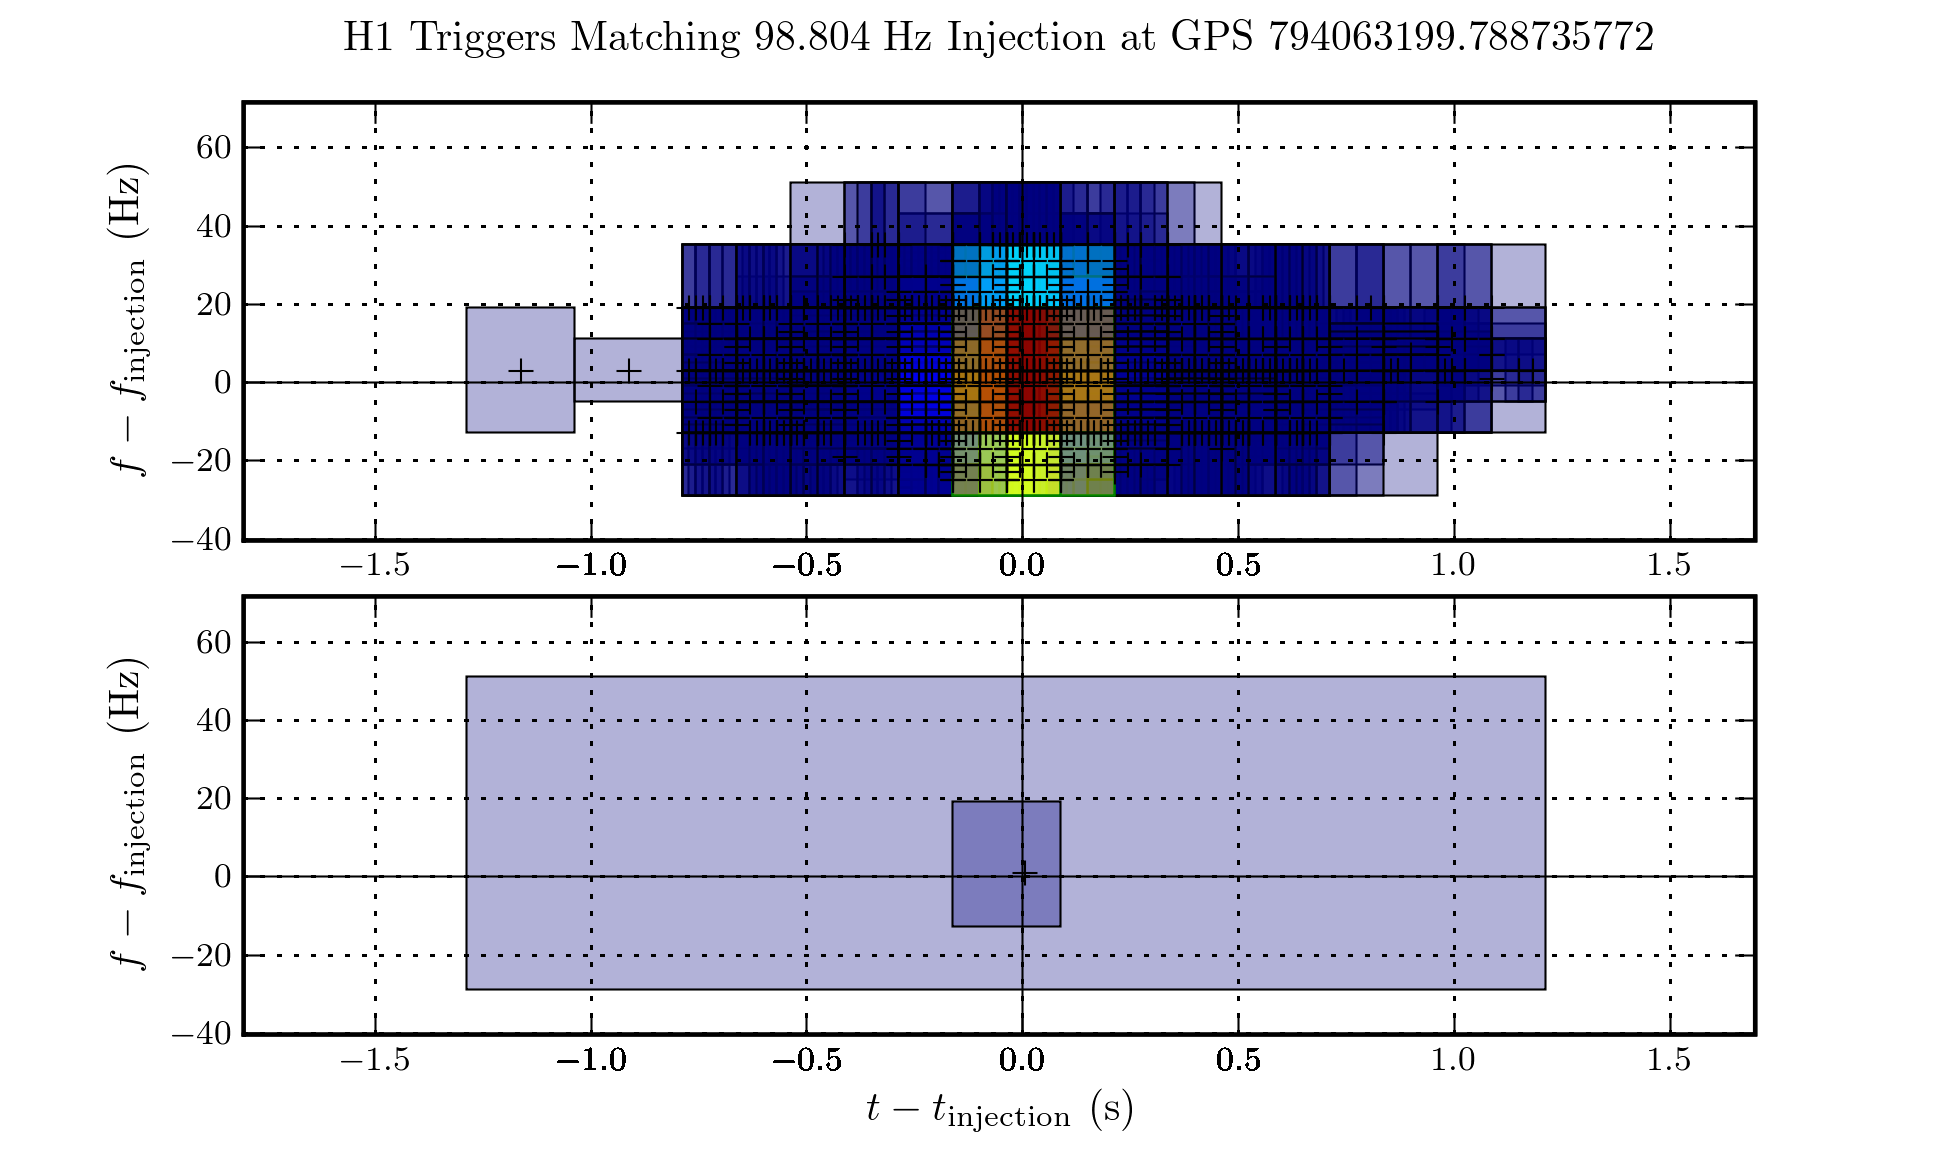
\includegraphics{figures/clustering_example.png}}
\end{center}
\caption{Example of excess power time-frequency triggers before and after
clustering.  Both panels show the trigger(s) resulting from a software
injection of a \(Q = 8.89\) sine-Gaussian, the horizontal axis is time
relative to the centre time of a software injection, and the vertical axis
is the frequency relative to the centre frequency of the injection.  The
top panel shows the many hundreds of triggers in the output of
\prog{lalapps\_power} resulting from this one software injection, the
bottom panel shows the single trigger in the output of
\prog{ligolw\_bucluster}.  The large rectangle marks the extent of the
triggers that formed the cluster, the small rectangle shows the ``most
significant portion'' of the event, and the small ``\(+\)'' marker
indicates the time and frequency where it is estimated the burst event's
energy peaked (note its proximity to the true centre time and frequency of
the injection).}
\label{fig2}
\end{figure}

\end{entry}


\section{Program \prog{ligolw\_cafe}}


\subsection{Overview}


The program \prog{ligolw\_cafe} (``coincidence analysis front end'') groups
trigger files for analysis in the coincidence stage of the pipeline.
Normally gravitational wave antennas do not have 100\% duty cycles, in
particular laser interferometers can frequently ``loose lock'' so that the
time series data recorded from the antenna has gaps in it.  This has the
side effect of providing natural boundaries in the data on which to divide
analysis tasks.  For example, if one has a collection of trigger files
gathered from two instruments and one wishes to search for coincident
events but there are gaps in the times spanned by the files, since events
stored in files before a gap cannot be coincident with events stored in
files after the gap one can avoid performing unnecessary comparisons in the
coincidence analysis by collecting together for coincidence tests only
events from within the same continguous group of files.  The program
\prog{ligolw\_cafe} is used to determine which files need to be grouped
together to perform a coincidence analysis among them.


\subsection{Operation}


This program takes as input a LAL cache file describing a collection of
files to be used in a coincidence analysis.  In particular, the instrument
and segment columns in the cache file should correctly describe the
contents of each file.  This program also uses for input a LIGO Light
Weight XML file containing a time\_slide table describing a list of
instrument and time delay combinations to be used in the coincidence
analysis.  The LAL cache files are named on the command line, or a cache
file can be read from stdin.  The time slide XML file is specified with a
command line option.

The program iteratively applies the time delays from the time\_slide table
in the time slide XML file to the segments of the files in the input cache.
For each time delay and instrument combination, the files whose segments
intersect one another are identified and placed together in groups, where
the files within a group intersect one another and the files in different
groups do not.  As different time delay and instrument combinations are
considered, the file groups are allowed to coalesce as needed.  The final
result is a collection of file groups, where no file from one group was
ever identified as being coincident with a file from another group in any
of the instrument and delay combinations considered.  Therefore, the
triggers from the files from one group need never be compared to the
triggers from the files in another group as it is known in advance that
they cannot be coincident.

The output of the program is a collection of LAL cache files, one LAL cache
for each coincident group of files that was identified.

One should think of this program as a coincidence analysis applied at the
level of entire files, whose role is to reduce the total number of
comparisons that need to be performed to complete the full coincidence
stage in a pipeline.


\section{Program \prog{ligolw\_burca}}


\subsection{Overview}


The program \prog{ligolw\_burca} actually performs two distinct functions.
In the future, it is likely these functions will be split into two
applications.  The first function performed by this program is an
inter-instrument coincidence comparison of the burst events stored in
sngl\_burst tables in LIGO light-weight XML files.  The other function
performed by this program is the ranking of \(n\)-tuples of
mutually-coincident events according to likelihood ratio data collected
from time-slide and injection runs.


\subsection{Coincidence Algorithm}


The coincidence tests applied by this application are exclusively two-event
tests:  one event from one instrument is compared to one event from another
instrument, and the two are either coincident or not.  Events taken from
more than two instruments constitute a coincident \(n\)-tuple when they are
all pair-wise mutually coincident.  Establishing the coincidence of an
\(n\)-tuple thus requires \(n\)-choose-2 tests, which scales as
\(\order(n^{2})\).  The total number of \(n\)-tuples that needs to be
tested is, in principle, \(\order(N^{n})\) where \(N\) is the average
number of events obtained from each instrument going into the coincidence
analysis.  A variety of optimization techniques are employed to avoid
unnecessary comparisons, but users should not be surprised to find that
this program can take a long time to run.

There are two coincidence tests to choose from.  These are as follows.
\begin{entry}
\item[excesspower]
Two events are coincident if their time-frequency tiles are not disjoint
after allowing for the light travel time between the two instruments.
There are no tunable parameters in this coincidence test, and the light
travel times are obtained from an internal look-up table of the locations
of known instruments.

When this coincidence test is selected, the output file has a multi\_burst
table added to it which is populated with summary information about each
coincident \(n\)-tuple identified by the coincidence analysis.  Each
coincident \(n\)-tuple is assigned an SNR equal to the square root of the
sum of the squares of the SNRs of the events that participate.  Each
\(n\)-tuple is also assigned a bandwidth, duration, and peak frequency
which are the \(\text{SNR}^{2}\)-weighted averages of the respective
quantities from the constituent events.  Each \(n\)-tuple is assigned an
\(h_{\text{rss}}\) equal to the \(h_{\text{rss}}\) of the most
statistically confident of the constituent events, and a confidence equal
to the lowest confidence of the constituent events.  At the present time,
of all of this information only the confidence assigned to the \(n\)-tuple
is used elsewhere in the pipeline.

\item[stringcusp]
Two events are coincident if their peak times do not differ by more than
\(\Delta t\) as set by the matching \option{--threshold} option from the
command line.  If the two events are taken from H1 and H2, then in addition
to the peak time comparison to be coincident they must also pass an
amplitude comparison.  Each string cusp burst event has an amplitude \(A\)
and an SNR \(\rho\), and the amplitude consistency test requires that
\begin{equation}
\magnitude{A_{1} - A_{2}}
   \leq \min \left\{ \magnitude{A_{1}} (\kappa / \rho_{1} + \epsilon),
   \magnitude{A_{2}} (\kappa / \rho_{2} + \epsilon) \right\},
\end{equation}
where \(\kappa\) and \(\epsilon\) are parameters supplied on the command
line.

\end{entry}

The results of the coincident event search are recorded in coinc tables in
the XML files, which are overwritten.


\subsection{Likelihood Ratio Analysis}


Setting the coincidence test to ``\option{excesspower2}'' switches to the
likelihood ratio analysis mode.  In this mode of operation,
\prog{ligolw\_burca} assigns likelihood ratios to the coincident
\(n\)-tuples it has previously identified using parameter distribution
density data collected from populations of time-slide (``noise'') and
injection (``gravitational wave'') \(n\)-tuples.  The procedure goes as
follows.  First, \prog{ligolw\_burca} is used to identify coincident
\(n\)-tuples in time-slide and injection trigger lists.  Another program,
\prog{ligolw\_burca\_tailor} (see Section \ref{section1}), scans these
\(n\)-tuples and collects summary statistics about their properties.
Finally, \prog{ligolw\_burca} is used to reprocess the \(n\)-tuples using
the parameter distributions measured by \prog{ligolw\_burca\_tailor} to
assign likelihood ratio values to each \(n\)-tuple, thereby ranking the
\(n\)-tuples from most to least injection-like.  Note that typically one
will not want to use the same \(n\)-tuples to assign likelihood ratio
values to themselves, but this is an unimportant operational detail at this
time.  See Figure \ref{fig3} for an example of the \(n\)-tuple parameter
distribution functions measured by \prog{ligolw\_burca\_tailor}.

Note that in likelihood ratio analysis mode, \prog{ligolw\_burca} processes
triggers in SQLite3 database files.  Use the program \prog{ligolw\_sqlite}
to transform LIGO Light Weight XML files into SQLite3 database files before
processing.


\section{Program \prog{ligolw\_binjfind}}


\subsection{Overview}


The program \prog{ligolw\_binjfind} processes LIGO light weight XML files
containing sim\_burst, sngl\_burst, and optionally coinc\_event tables and
identifies and records which burst events correspond to injections.  There
are three kinds of burst/injection matches that are searched for and
recorded:
\begin{itemize}
\item individual burst events in the sngl\_burst table that match
injections in the sim\_burst table,

\item coincident \(n\)-tuples of burst events that match ``exactly''
injections in the sim\_burst table,

\item and coincident \(n\)-tuples of burst events that are ``nearby''
injections in the sim\_burst table.
\end{itemize}
Two burst/injection comparison tests are available, one for use with the
excess power burst search pipeline and one for use with the string cusp
search pipeline.  An ``exact'' \(n\)-tuple/injection match is one in which
every burst event in the coincident \(n\)-tuple is identified as matching
the injection according to the burst/injection comparison test.  A
``nearby'' \(n\)-tuple/injection match is a coincident \(n\)-tuple of burst
events that occurs within \(\unit{2}{\second}\) of the injection (the
injection does not precede the first of the events' start times or lag the
last of their end times by more than \(\unit{2}{\second}\)).

The reason for the two distinct types of \(n\)-tuple/injection matches is
that there are two reasons one wishes to identify an injection in a list of
burst events.  On the one hand, one wishes to characterize the search code
in order to measure how well it does or does not recover the parameters of
an injection and for this one does not want to be distracted by accidental
injection recoveries (when noise in the time series happens to occur near
an injection), and so one wishes to identify burst events that really are
believed to be the direct result of the software injection.  On the other
hand, one wishes to measure the detection efficiency of the pipeline or the
probability that the pipeline produces a detection candidate when a
software injection is placed in the time series.  In this case it doesn't
matter if the injection is recovered well at all, only whether or not
something (anything) survives the pipeline when the injection is placed in
the input.

The results of the injection identification tests are recorded in the coinc
tables in the XML files, which are overwritten.


\section{Program \prog{ligolw\_burca\_tailor}}
\label{section1}


\subsection{Overview}


The program \prog{ligolw\_burca\_tailor} scans the coincident \(n\)-tuples
of burst events recorded in LIGO Light Weight XML files and collects
statistics on their properties.  The resulting parameter distribution
densities are written as Array data to LIGO Light Weight XML files which
can be used by \prog{ligolw\_burca} to assign likelihood ratio values to
coincident \(n\)-tuples.

Note that \prog{ligolw\_burca\_tailor} operates on SQLite3 database files.
Use the program \prog{ligolw\_sqlite} to transform LIGO Light Weight XML
into SQLite3 database files before processing with
\prog{ligolw\_burca\_tailor}.


\subsection{Operation}


This program collects statistics specific to the excess power burst search
pipeline.  At present, the events in an \(n\)-tuple are taken pair-wise and
5 parameters computed for each pair:
\begin{itemize}
\item \((\Delta t_{1} - \Delta t_{2}) / \mean{\Delta t}\), the difference
in the two events' ``most significant'' durations as a fraction of the
average of the two durations,

\item \((\Delta f_{1} - \Delta f_{2}) / \mean{\Delta f}\), the difference
in the two events' ``most significant'' bandwidths as a fraction of the
average of the two bandwidths,

\item \((h_{\text{rss}_{1}} - h_{\text{rss}_{2}}) /
\mean{h_{\text{rss}}}\), the difference of the two events'
\(h_{\text{rss}}\)s as a fraction of the average of the two,

\item \((f_{1} - f_{2}) / \mean{f}\), the difference of the two events'
peak frequencies as a fraction of the average of the two,

\item \(t_{1} - t_{2}\), the difference in the two events' peak times.

\end{itemize}
The first four quantities are dimensionless and algebraically confined to
the interval \([-2, +2]\).  The fifth parameter is dimensionful and has no
natural interval in which its values are confined.  A three-event
\(n\)-tuple is characterized by a total of 15 parameters, one set of the
five numbers above for each choice of two events from the \(n\)-tuple.

The parameter distributions are tracked by constructing bins, and for each
bin counting how many \(n\)-tuples produce a parameter value in the range
represented by that bin.  When all the \(n\)-tuples have been processed,
the bin counts are stored as Array data in an output LIGO Light Weight XML
file.  For the parameters confined to finite intervals, the distributions
are measured using simple linearly-spaced bins.  For the \(t_{1} - t_{2}\)
parameters a non-linear binning is used in which the bins are uniform in
\(\tan^{-1} [(t_{1} - t_{2}) / T]\), where \(T\) is a parameter used to set
the scale of the bins.  This binning produces bins that are approximately
uniformly spaced for small \((t_{1} - t_{2}) / T\), but transition to
asymptotically diminishing density for large \((t_{1} - t_{2}) / T\).

Figure \ref{fig3} shows an example of the parameter distributions measured
for time-slide and injection \(n\)-tuples in stationary Gaussian noise.
\begin{figure}
\begin{center}
\resizebox{.9\linewidth}{!}{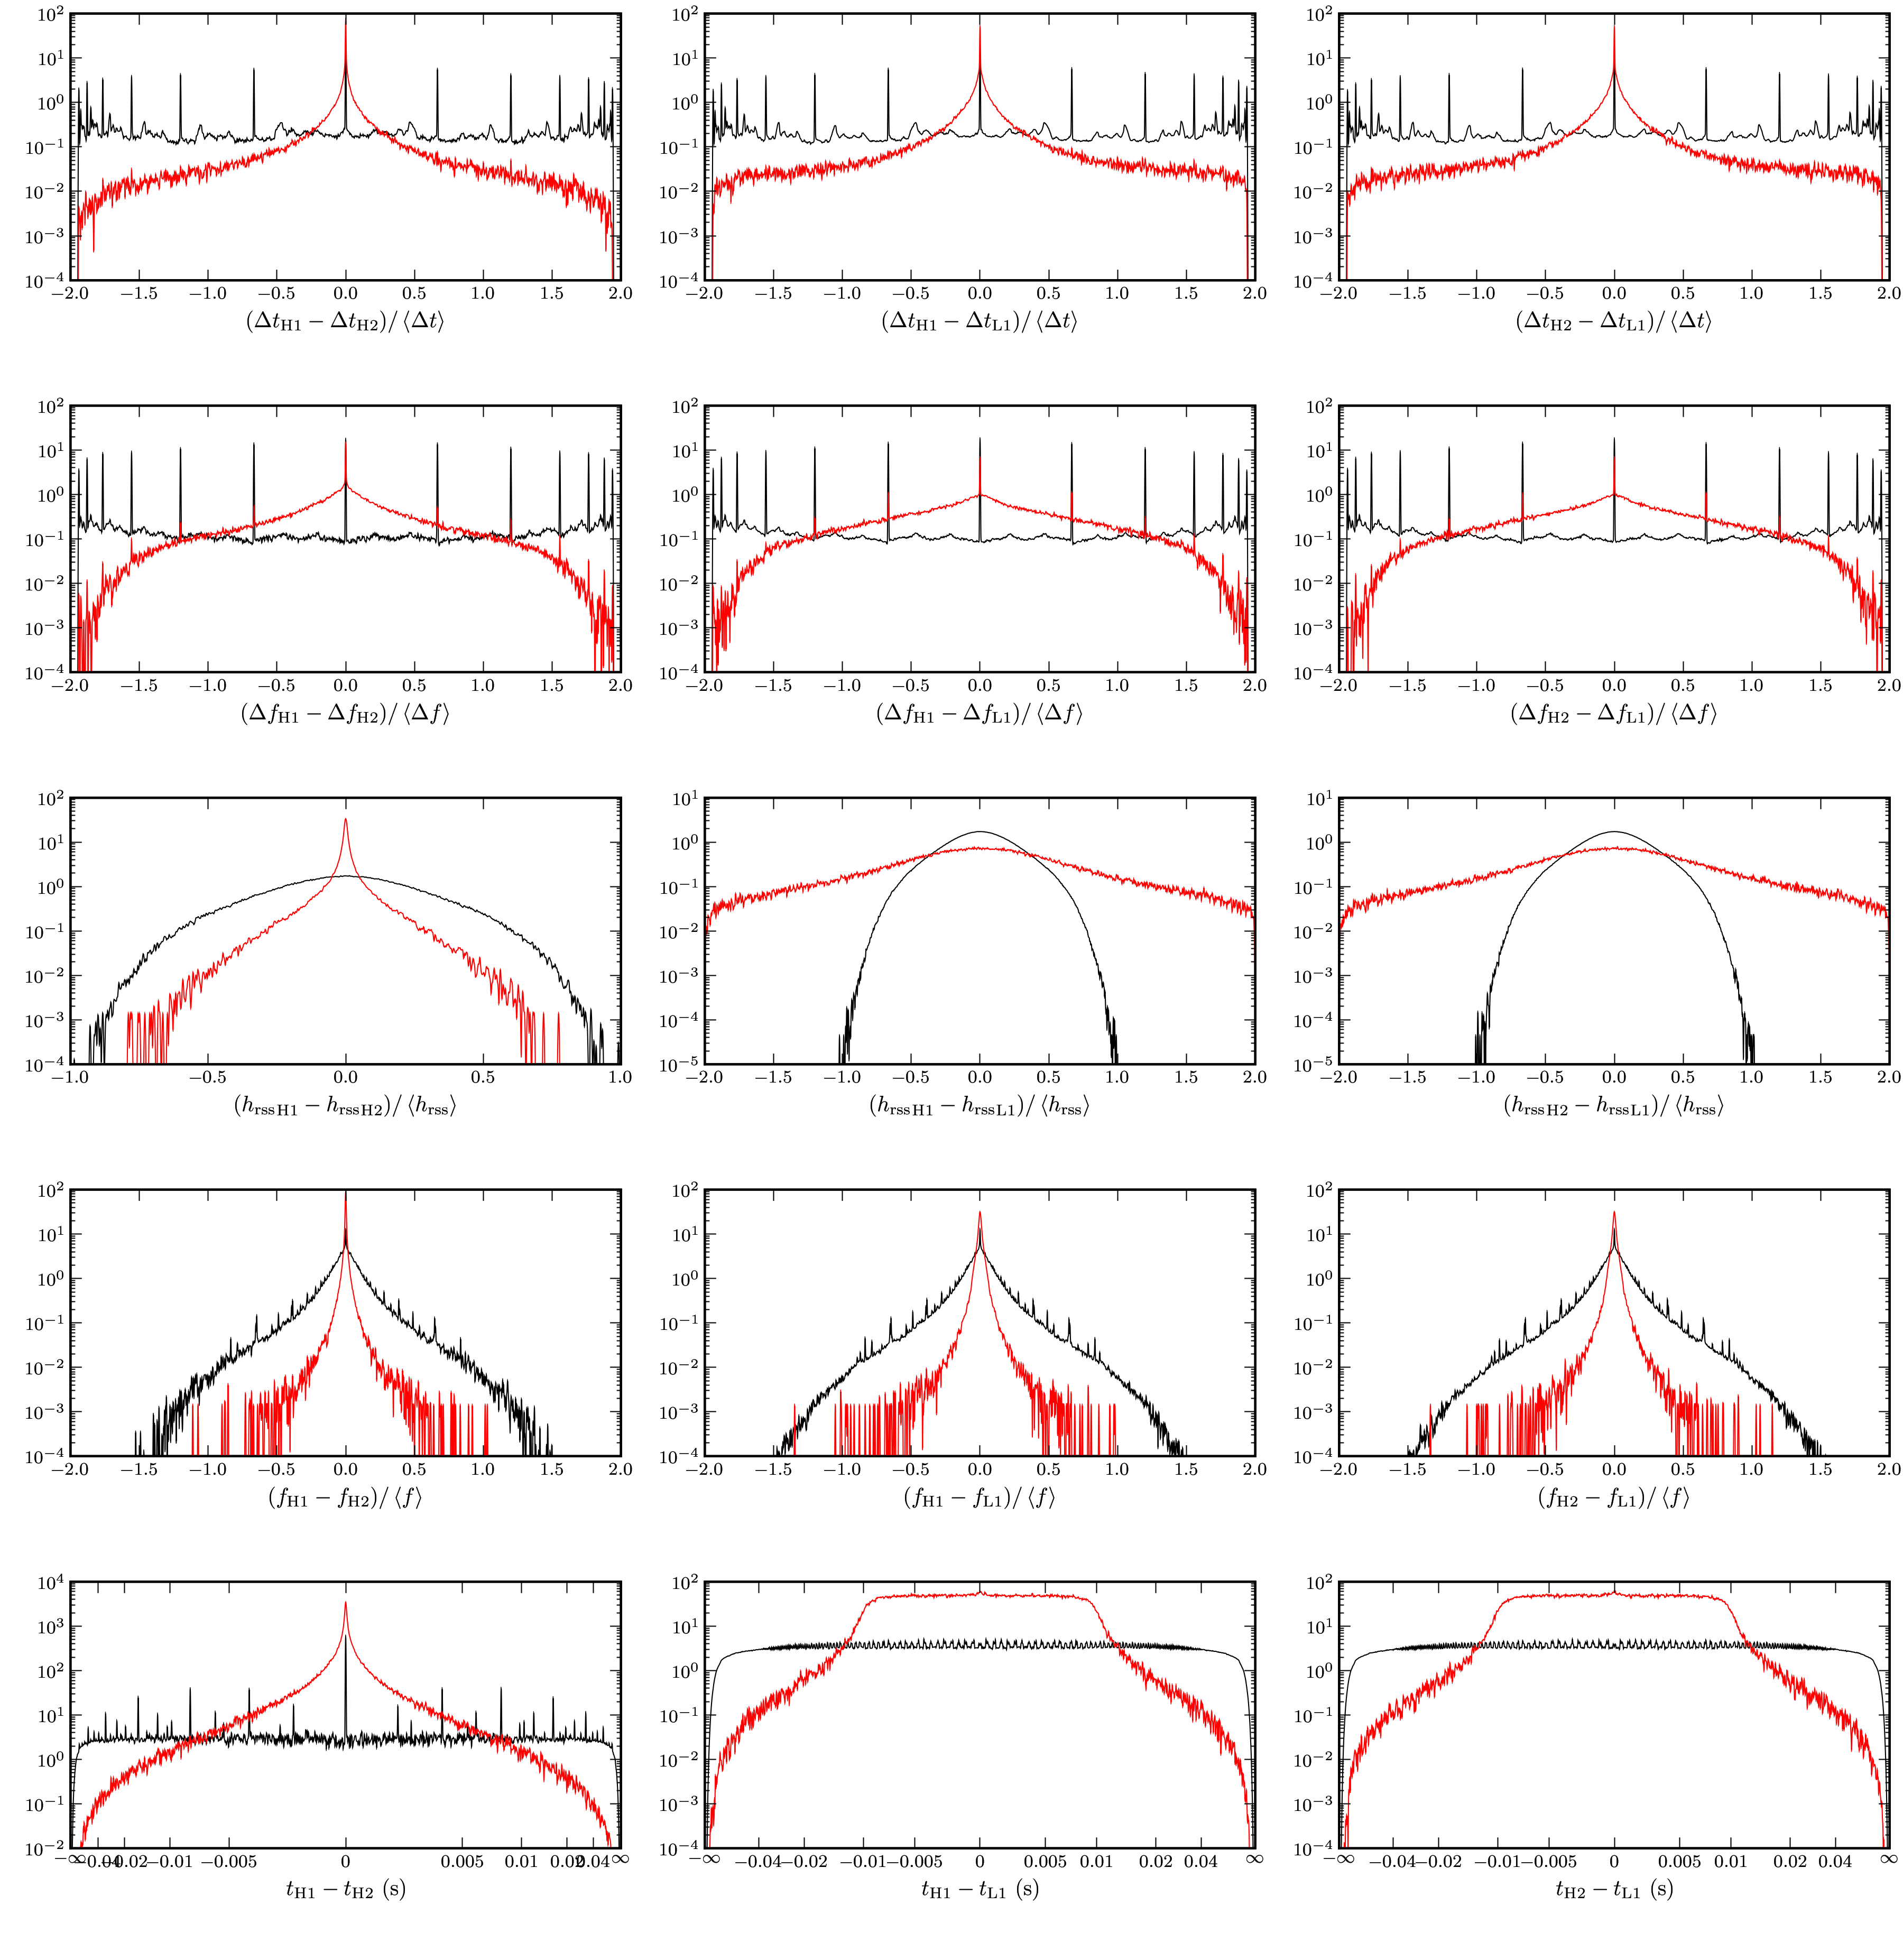
\includegraphics{figures/plotburca2-P-793154128-2525061.png}}
\end{center}
\caption{Example of the parameter distributions collected by
\prog{ligolw\_burca\_tailor}.  The black curves are the distributions
observed in time-slide \(n\)-tuples (``noise''), and the red are the
parameter distributions observed in software injection \(n\)-tuples
(``gravitational waves'').}
\label{fig3}
\end{figure}


\subsection{Other Features}


The program \prog{ligolw\_burca\_tailor} can also merge LIGO Light Weight
XML files containing distribution data into single files.  The collection
of the statistics can be a time-consuming operation, and it can be
convenient to process files in parallel groups on a compute cluster.  In
this case, it's necessary to be able to merge the bin counts after each
group of trigger files has been processed.


\section{Program \prog{ligolw\_tisi}}
\label{section3}


% FIXME

Blah blah blah.


\section{Pipeline Construction}
\label{section2}


\subsection{Overview}


The ``excess power pipeline'' is the search pipeline that results from
chaining the programs described above together to perform a
multi-instrument search for gravitational wave bursts.  Typically the
pipeline is executed on a Condor compute cluster (this is the only mode
that has been tested).  This is done using a set of Condor job control
files which instruct Condor as to the sequence of jobs to run and the
command line arguments to give each.  The Condor control files are
generated using a set of Python scripts described below.

Refering to the pipeline schematic in Figure \ref{fig1}, there are two
scripts for building the excess power pipeline.  The first script,
\prog{lalapps\_power\_pipe}, builds the ``top half'' of the pipeline, the
part of the pipeline above the dashed divider in the schematic.  This part
of the pipeline involves data discovery, optional software injections,
trigger identification, clustering, coincidence analysis, and injection
identification.  The second script,
\prog{lalapps\_power\_likelihood\_pipe}, builds the ``bottom half'' of the
pipeline.  In this part of the pipeline, coincident \(n\)-tuple parameter
distribution data is used to rank coincidences according to how
injection-like they appear.

In the top half of the pipeline, all programs manipulate data files in LIGO
Light Weight XML format.  In the bottom half, all programs manipulate the
data files in SQLite3 database format.  The transition from XML to SQLite3
occurs at the end of the top half of the pipeline, where the data
processing sequence ends with a set of \prog{ligolw\_sqlite} jobs to
convert the files.

The Condor control files for the top and bottom halves of the pipeline can
reside in the same directory (there are no name conflicts), so the entire
pipeline can be constructed as a pair of DAGs in a single directory.


\subsection{The Pipeline's Top Half}


The Condor control files for the pipeline's top half are constructed using
the program \prog{lalapps\_power\_pipe}.  This program can generate three
versions of the pipeline's top half:  a version containing the
non-injection portion of the pipeline only (the left part of Figure
\ref{fig1}), a version containing the injection portion of the pipeline
only (the right part of Figure \ref{fig1}), or a version containing both
injection and non-injection jobs.

To generate the Condor control files, the pipeline construction program
\prog{lalapps\_power\_pipe} requires the following information as input.
\begin{itemize}
\item One or more LIGO Light Weight XML files containing one time\_slide
table each (See \prog{ligolw\_tisi} in Section \ref{section3}) describing
the instrument and time delay combinations to use in the non-injection
coincidence stage of the pipeline.  These files are not required if the
injection-only version of the pipeline is being constructed.  Each time
slide file results in a separate set of \prog{ligolw\_burca} jobs being
constructed.  This allows a large number of time slides to be analyzed,
distributing them across multiple \prog{ligolw\_burca} jobs.

\item One LIGO Light Weight XML file containing the time\_slide table
identifiying the instrument and delay combinations to be used in the
injection coincidence stage of the pipeline.  This file is not required if
the non-injection only version of the pipeline is being constructed.  Note
that at the present time, the injection stage of the pipeline can only
process injections at 0 offset so only all-zero time slides can be given in
this input file.  However, the instrument combination appearing in the time
slides are used to determine which pairs of instruments to combine in the
coincidence stage.

\item A set of files in segwizard format listing the segments to be
analyzed.  There must be exactly one segment file for each instrument
appearing in any of the time slides found in the time slide files.

\item A .ini file providing miscellaneous configuration information for the
pipeline construction script.  In particular, the command line options used
used for each program are given in this file as well as the names of the
segment files and the executables to use.

\end{itemize}

The pipeline script analyzes the segments and the time slides and
determines which time intervals can be analyzed, and which time intervals
will be combined together for the coincidence analyses.  Instances of
\prog{lalapps\_power} are used to generate triggers, and
\prog{ligolw\_bucluster} jobs are used to cluster the resulting triggers.
The program \prog{ligolw\_add} is used to combine the appropriate trigger
files together in preparation for coincidence analysis.  At this time, the
time slides files generated by the user prior to pipeline construction are
also merged into the trigger files, and in the case of the injection branch
of the pipeline the list of software injections is also merged into the
trigger file.  The resulting merged data files are processed with
\prog{ligolw\_burca} for coincidence identification, and in the case of the
injection portion of the pipeline with \prog{ligolw\_bucut} and
\prog{ligolw\_binjfind} to trim the software injection list and identify
software injections respectively.  Finally, a set of \prog{ligolw\_sqlite}
jobs convert the XML files to SQLite3 database files.  A representative
graph of the parent-child relationships among the jobs is shown in Figure
\ref{fig4}
\begin{figure}
\begin{center}
% FIXME
FIXME
\end{center}
\caption{A graph showing the parent-child relationships among the jobs in
the top half of the excess power pipeline.}
\label{fig4}
\end{figure}


\section{Tuning the Excess Power Pipeline}


The excess power search identifies time-frequency tiles as events when the 
probability of getting power in the tile from Gaussian noise alone
is below some particular threshold.  The search assumes no particular 
information about the gravitational wave signals other than the time
frequency ranges to search for,  so once those ranges are chosen the main 
tool to tune the pipeline is by tweaking the threshold.  The other parameter 
to test in the tuning procedure is the coincidence window.  Thus to 
summarize the parameters to tune in the excess power search are:
\begin{itemize}
\item maximum duration(seconds) of the tiles
\item maximum bandwidth of the tiles
\item probability thresholds on the individual instruments
\item the coincidence window
\end{itemize}
In the following sections we will go over the tuning of the different 
parameters in more details.


\subsection{Tuning the size of the tiles}
\label{section:tunetilesize}


The size(duration and bandwidth) of the tiles are largely guided by the
time-frequency content of the gravitational waves one is searching for.
  Here,  we describe the tuning procedure where we were concentrating 
on the search of the merger phase preceded by an inspiral phase.  As
mentioned before the physical parameters describing the merger phase
of a binary black hole coalescence are very poorly understood till
today.  However there are some rough estimates available in the literature 
which we will briefly describe here.  These will provide us a guideline
in choosing the parameters of our search pipeline. [FH:Flannagan and Hughes]

The process of coalescence can be roughly divided into three phases:
\begin{itemize}
\item Inspiral phase
\item Merger phase
\item Ringdown phase
\end{itemize}
The inspiral phase can be modelled accurately enough to use the match
filtering techniques to search for the waveforms, however for massive
black holes when there are not enough cycles left in the inspiral phase 
we have to rely on the merger phase for the detection of the coalescence.
According to the estimates of FH, binary black hole systems with total
mass $M \leq 30M_{\odot}$ are best searched for via their inspiral waves
while systems with $M > 30M_{\odot}$ must be searched via their
merger waves and/or their well understood ringdown waves.  

FH has estimated a conservative value for the merger frequency given
by 
\begin{equation}
f_{merge} = \frac{0.02}{M} \\
          = 205 Hz (\frac{20M_{\odot}}{M})
\label{eq:fmerge}
\end{equation}.
This is conservative in the sense that one can reasonably be sure that
numerically generated templates will not be needed before $f = f_{merger}$.
Now LIGO noise floor restricts the lowest frequency that can be searched 
for and in $S4$ this is $\approx 50 Hz$. Using \eqref{eq:fmerge} we 
then get that a binary system of maximum mass $\approx 80M_{\odot}$ 
can be searched for in $S4$.  However for a $80 M_{\odot}$ binary the 
number of cycles in the inspiral phase will be very small and since we
are interested in the coincidence of the mergers with the inspirals we
would like to restrict our search to a bit lower total mass.  Thus the 
mass range of the binary black holes that we decide to look at for the 
IB search is given by 
\begin{equation}
30 M_{\odot} < M \leq 70 M_{\odot}. 
\label{eq:massrange}
\end{equation}
Given this mass range let us now see what can we estimate about the 
expected frequency and duration of the merger signals. From 
\eqref{eq:fmerge} we get the approximte range of the merger frequencies:
\begin{equation}
58 Hz < f_{merge} \leq 140 Hz
\label{eq:frange}
\end{equation}
Now according to FH the high frequency shut off for the mergers are
roughly given by 
\begin{equation}
f_{qnr} = 1320 Hz (\frac{20M_{\odot}}{M})
\label{eq:fqnr}
\end{equation}
Thus if the assumed bandwidth of the merger signal is 
$\Delta f = f_{qnr} - f_{merge}$,  then for our mass range of 
interest we may expect the bandwidth to be of the order of few
hundred Hertz.  

The effective duration for the signals has also been roughly estimated
by FH to be:
\begin{equation}
50 M < T < 10 M
\label{eq:timerange}
\end{equation}
depending on the total spin of the binary system. If we consider
a coalescence where both the inspiraling black holes are nearly
maximally spinning, with their spins and the orbital angular momentum
nearly alligned then the merger may be expected to be long,  while
for non-spinning black holes the merger will be rather quick.  Thus 
given our mass range of interest (\eqref{eq:massrange}) the 
time duration of the expected signals whould be somewhere in the 
range:
\begin{equation}
17.2 ms < T < 1.5 ms
\label{eq:trange}
\end{equation} 
  
So given these estimates about the bandwidth and the duration of the 
signals of our main interest we choose the following parameters in our
search pipeline:
\begin{itemize}
\item Low frequency cutoff: $50 Hz$
\item Bandwidth: $1024 Hz$
\item Maximum duration of a tile: $125 ms$; we have set the duration 
a few times longer than the maximum duration in \eqref{eq:trange}
because of the uncertainty in the estimations related to the nature 
of the merger signals.
\item Maximum bandwidth of a tile: $128 Hz$; we have the bandwidth 
smaller than the estimated bandwidths for the merger signals since
because of the LIGO noise curve the prominent contribution to the 
power from the merger phase will be for a few hundred Hertz.
\end{itemize}
The last two parameters set the maximum duration and bandwith of 
a single tile in the search,  which does not preclude us from searching
for longer or broader signals since we can always sum up the power
from multiple tiles triggered by the particular signal. 
    

\subsection{Deciding on the probability thresholds}


We saw in Sec~\ref{section:tunetilesize} that the sizes of the tiles
are mainly guided by the rough expectations about the signals that 
we are interested in.  However, the threshold on the probability
of power in a tile is guided by the optimisation between the false 
rate and efficiency to a set of Monte Carlo simulations.  The idea
we usually follow is to choose a threshold which lowers the false rate 
maintaining the efficiency at an acceptable value.

To get a rough idea about the region where we start loosing significant 
amount of efficiency without an appreciable effect in lowering the false 
rate we estimate the efficiencies and the false rates for a number of 
thresholds. We have used $Q9$ Sine-Gaussian waveforms at $235 Hz $ to
perform the tuning and the confidence thresholds are
$\{-30.0, -35.0, -40.0, -45.0, -50.0, -55.0, -60.0, -65.0, -70.0, -80.0, 
-90.0, -100.0, -150.0, -200.0\}$. How the efficiency and the false rate 
depend on the thresholds are shown in Fig~\ref{fig:dt125df128tune}: 
\begin{figure}
\begin{center}
\resizebox{.9\linewidth}{!}{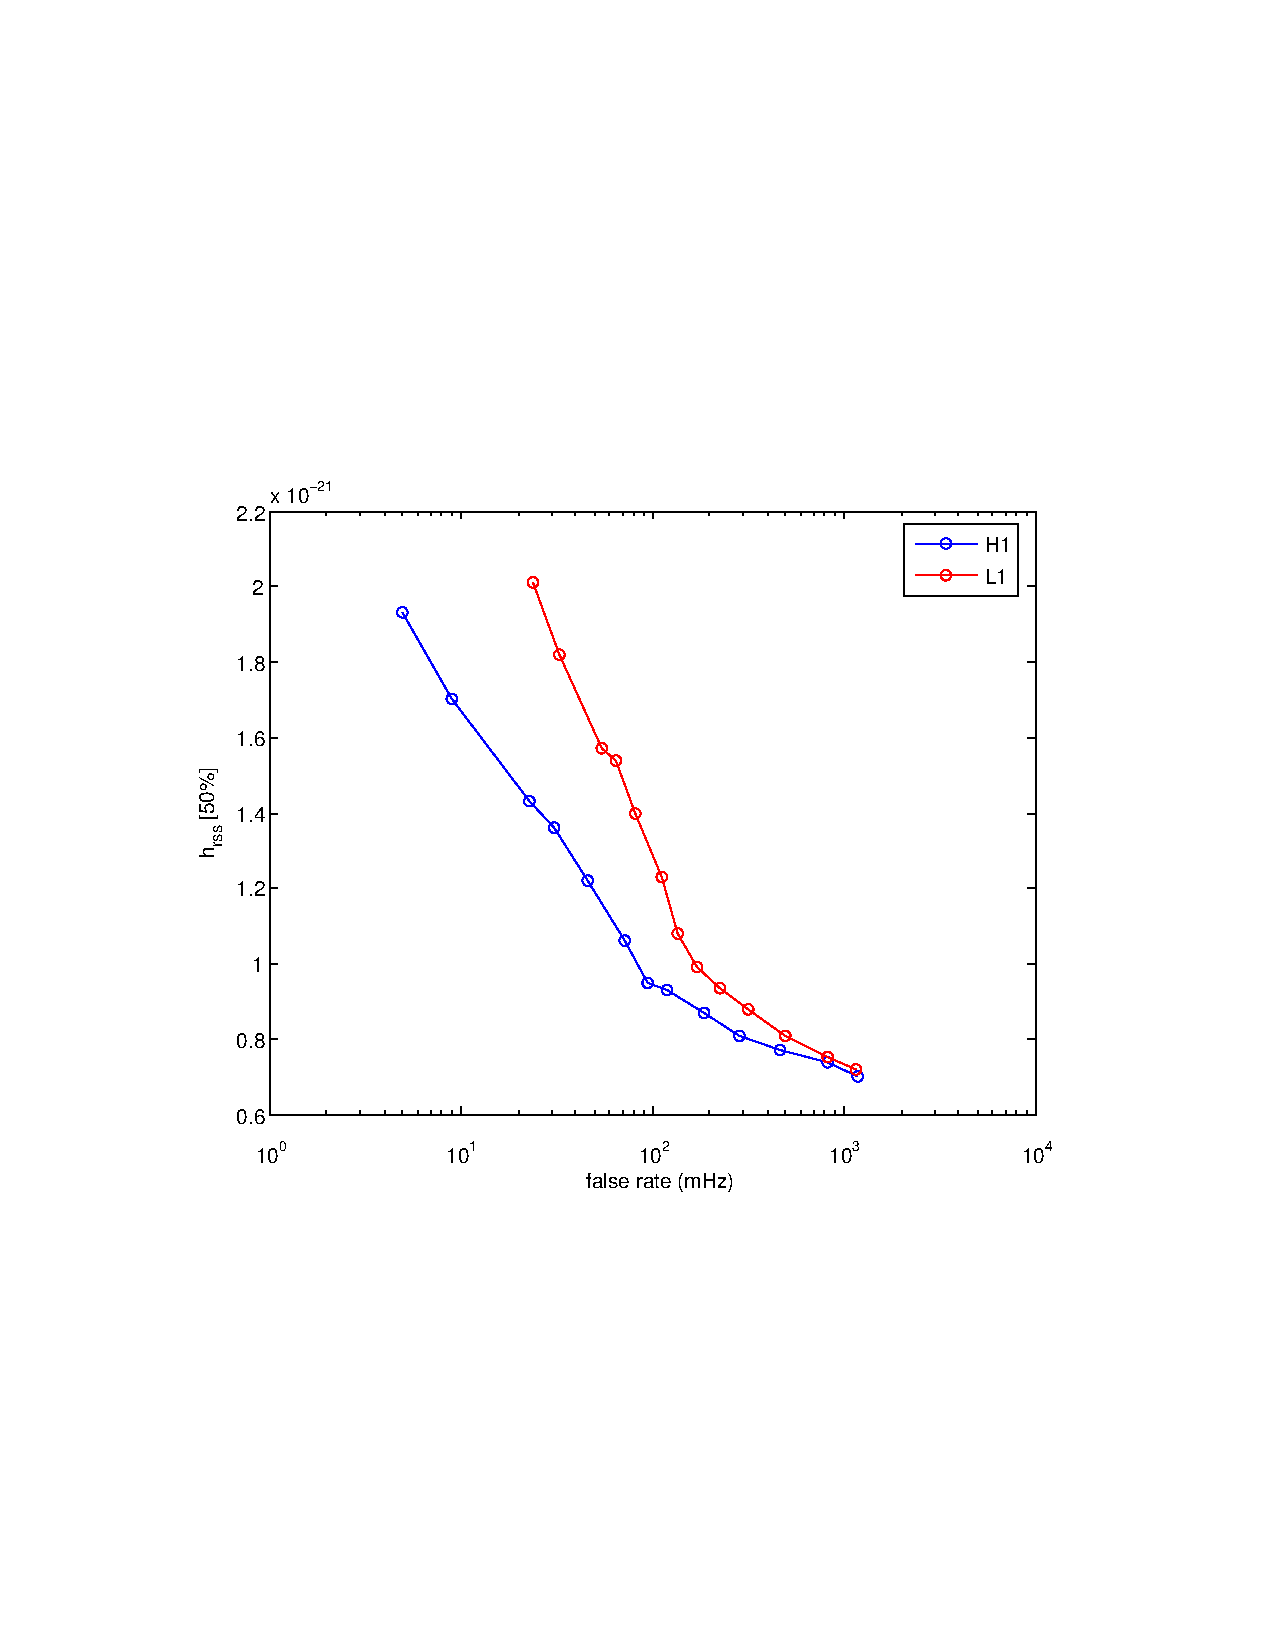
\includegraphics{figures/H1_L1_dt125_df128}}
\caption{Efficiency vs. False rate for different |thresholds|}
\label{fig:dt125df128tune}
\end{center}
\end{figure}
The circles on the curves show the values corresponding to different 
thresholds.  The maximum false rate and the best efficiency are obtained 
for the lowest |threshold|(30.0),  then as the |threshold| is increased
the false rate decreases while the efficiency gets worse. Around the 
|thresholds| of $50.0 - 60.0$ one may notice that for a very small 
decrease in false rate the efficiency gets a whole lot worse.  This gives 
us a rough idea that we should choose $ |threshold| < 60.0$.  However
one should be aware of the fact that tuning must be specific to the 
pipeline being run.  In our pipeline we have a coincidence step which
involves the burst triggers and the inspiral triggers and we are not
quite sure how many of the false triggers will survive that step. We
also plan to use the Hanford 2Km instrument in a coherent follow up at
the end of the pipeline which will also hopefully get rid off many of the
false triggers. However we would like to  
have a good estimate of the background distribution of triggers and so 
have a few surviviors at the end of the pipeline.  Keeping that 
in mind we decided to choose a looser threshold on the confidence 
probabilities. The thresholds we chose are 
\begin{itemize}
\item Threshold on H1: -38.0
\item Threshold on L1: -38.0; The instrument in Livingstone was less 
sensitive than the one in Hanford for the first half of the run but 
for the second half both the instruments had equal sensitivity.  So
we decided to have the same thresholds on both the instruments.
\end{itemize}      
These thresholds were so chosen so that the false rate after 
coincidence between H1 and L1 triggers is $\approx 2 mHz$ while 
the $ h_{rss}$ is $\approx 1.12e-21$.


\bibliography{refs}


\end{document}
